%% ----------------------------------------------------------------
%% Thesis.tex -- MAIN FILE (the one that you compile with LaTeX)
%% ---------------------------------------------------------------- 

% Set up the document
\documentclass[a4paper, 11pt, oneside]{Thesis}  % Use the "Thesis" style, based on the ECS Thesis style by Steve Gunn
\graphicspath{Figures/}
% Include any extra LaTeX packages required
\usepackage{mathrsfs}
\usepackage{hyperref}
\usepackage{algorithm}
\usepackage[inline]{enumitem}
\usepackage{algpseudocode}
\usepackage{bbold}
\usepackage[square, numbers, comma, sort&compress]{natbib}  % Use the "Natbib" style for the references in the Bibliography
\usepackage{verbatim}  % Needed for the "comment" environment to make LaTeX comments
\usepackage{vector}  % Allows "\bvec{}" and "\buvec{}" for "blackboard" style bold vectors in maths
\usepackage{tikz}
\usepackage{tikz-network}
\usepackage{booktabs}
\usepackage{placeins}

\usetikzlibrary{fit, positioning, arrows.meta}
\hypersetup{urlcolor=blue, colorlinks=true}  % Colours hyperlinks in blue, but this can be distracting if there are many links.

%% ----------------------------------------------------------------
\begin{document}
\frontmatter      % Begin Roman style (i, ii, iii, iv...) page numbering

% Set up the Title Page
\title  {Thesis Title}
\authors  {\texorpdfstring
            {\href{your web site or email address}{Author Name}}
            {Author Name}
            }
\addresses  {\groupname\\\deptname\\\univname}  % Do not change this here, instead these must be set in the "Thesis.cls" file, please look through it instead
\date       {\today}
\subject    {}
\keywords   {}

%\maketitle

%% ----------------------------------------------------------------
%% ----------------------------------------------------------------



\setstretch{1.3}  % It is better to have smaller font and larger line spacing than the other way round

% Define the page headers using the FancyHdr package and set up for one-sided printing
\fancyhead{}  % Clears all page headers and footers
\rhead{\thepage}  % Sets the right side header to show the page number
\lhead{}  % Clears the left side page header

\pagestyle{fancy}  % Finally, use the "fancy" page style to implement the FancyHdr headers


\begin{titlepage}
\begin{center}
 
\Large\textbf{Department of Physics and Astronomy\\
University of Heidelberg}

\vspace{13cm}

\normalsize
Master Thesis in Physics\\
submitted by\\
\vspace{0.5cm}
\Large\textbf{Eric Niklas Willi Volkmann}\\
\normalsize
\vspace{0.5cm}
born in Waldems Esch (Germany)\\
\vspace{0.5cm}
\Large\textbf{2023}
\normalsize

\newpage
	\thispagestyle{empty}
\phantom{blabla}
\newpage



\Large\textbf{BOLD observation model for the dynamical systems reconstruction of fMRI time series}

\vspace{15cm}

\normalsize
This Master Thesis has been carried out by Eric Volkmann at the\\
Central Institute of Mental Health Mannheim\\
under the supervision of\\
Prof. Dr. Daniel Durstewitz
\thispagestyle{empty}
\vfill
\end{center}

\end{titlepage}

%% ----------------------------------------------------------------
% Declaration Page required for the Thesis, your institution may give you a different text to place here
%\Declaration{

%\addtocontents{toc}{\vspace{1em}}  % Add a gap in the Contents, for aesthetics

%I, AUTHOR NAME, declare that this thesis titled, `THESIS TITLE' and the work presented in it are my own. I confirm that:

%\begin{itemize} 
%\item[\tiny{$\blacksquare$}] This work was done wholly or mainly while in candidature for a research degree at this University.
 
%\item[\tiny{$\blacksquare$}] Where any part of this thesis has previously been submitted for a degree or any other qualification at this University or any other institution, this has been clearly stated.
 
%\item[\tiny{$\blacksquare$}] Where I have consulted the published work of others, this is always clearly attributed.
 
%\item[\tiny{$\blacksquare$}] Where I have quoted from the work of others, the source is always given. With the exception of such quotations, this thesis is entirely my own work.
 
%\item[\tiny{$\blacksquare$}] I have acknowledged all main sources of help.
 
%\item[\tiny{$\blacksquare$}] Where the thesis is based on work done by myself jointly with others, I have made clear exactly what was done by others and what I have contributed myself.
%\\
%\end{itemize}
 
 
%Signed:\\
%\rule[1em]{25em}{0.5pt}  % This prints a line for the signature
 
%Date:\\
%\rule[1em]{25em}{0.5pt}  % This prints a line to write the date
%}
%\clearpage  % Declaration ended, now start a new page

%% ----------------------------------------------------------------
% The "Funny Quote Page"
%\pagestyle{empty}  % No headers or footers for the following pages

%\null\vfill
% Now comes the "Funny Quote", written in italics
%\textit{``Write a funny quote here.''}

%\begin{flushright}
%If the quote is taken from someone, their name goes here
%\end{flushright}

%\vfill\vfill\vfill\vfill\vfill\vfill\null
%\clearpage  % Funny Quote page ended, start a new page
%% ----------------------------------------------------------------

% The Abstract Page
%\addtotoc{Abstract}  % Add the "Abstract" page entry to the Contents
%\abstract{
%\addtocontents{toc}{\vspace{1em}}  % Add a gap in the Contents, for aesthetics

%The Thesis Abstract is written here (and usually kept to just this page). The page is kept centered vertically so can expand into the blank space above the title too\ldots

%}

%\clearpage  % Abstract ended, start a new page


%% ----------------------------------------------------------------

\setstretch{1.3}  % Reset the line-spacing to 1.3 for body text (if it has changed)

% The Acknowledgements page, for thanking everyone
%\acknowledgements{
%\addtocontents{toc}{\vspace{1em}}  % Add a gap in the Contents, for aesthetics

%The acknowledgements and the people to thank go here, don't forget to include your project advisor\ldots

%}
%\clearpage  % End of the Acknowledgements
%% ----------------------------------------------------------------

\pagestyle{fancy}  %The page style headers have been "empty" all this time, now use the "fancy" headers as defined before to bring them back

\lhead{\emph{Abstract}}
\begin{Abstract}
    The reconstruction of dynamical systems underlying observed time series is a common task across many scientific disciplines. One tool developed 
    to accomplish this task is the piecewise linear recurrent neural network (PLRNN) with its universal approximation capabilities trained using 
    backpropagation through time (BPTT) and teacher forcing. Because of it is mathematical tractable, a trained PLRNN allows for a simple DS analysis 
    after it has been successfully trained on a system. \newline
    This thesis aims to apply this PLRNN training framework to functional magnetic resonance imaging (fMRI), which measures brain activity via the 
    bold-oxygen-level dependent contrast, i.e. the BOLD signal. To this end, a BOLD observation model, that models the hemodynamic response in the 
    BOLD signal, is developed in this thesis as well as the inversion algorithm for the BOLD observation needed for teacher forcing. The PLRNN with the
    BOLD observation model is then first benchmarked on an artificial Lorenz63 benchmark and then applied to the LEMON 
    ("Leipzig Study for Mind-Body-Emotion Interactions") dataset. While the benchmark results appear very promising, the application to real fMRI
    time series remains challenging.
\end{Abstract}

\begin{center}%
  \bfseries{Zusammenfassung} 
\end{center}
  Die Rekonstruktion dynamischer Systeme aus observierten Zeitreihen ist über viele wissenschaftliche Disziplinen hinweg eine häufige Aufgabe.
  Ein Werkzeug um dieses Problem zu lösen sind stückweise lineare rekurrente neuronale Netzwerke (PLRNN) mit ihren universalen Approximationsfähigkeiten.
  Sie werden mittels des Algorithmus "backpropagation through time (BPTT)" und "teacher forcing" (TF) trainiert. Aufgrund ihrer mathematischen Form 
  erlauben PLRNNs eine einfache Analyse der rekonstruierten Systeme nach dem Training. \newline

  In dieser Arbeit wird das PLRNN Trainingsframework auf Zeitreihen aus der funktionelle Magnetresonanztomografie (fMRT), welche die Gehirnaktivität 
  basierend auf der Blutoxygenierung, dem BOLD Signal, misst, angewendet. Dazu wird eine BOLD Beobachtungsmodell entwickelt, welches die neurovaskuläre
  Kopplung im BOLD Signal modelliert, und der dazugehörige Umkehralgorithmus, der für das Training mit TF notwendig ist. Das PLRNN mit dem BOLD
  Beobachtungsmodell wird zunächst auf einem künstlichen Datensatz basierend auf dem Lorenz63 getestet und dann auf den LEMON
  ("Leipzig Study for Mind-Body-Emotion Interactions") Datensatz angewandt. Während die Ergebnisse auf dem Lorenz System sehr vielversprechend sind,
  zeigen sich weiterhin viele Schwierigkeiten auf dem LEMON Datensatz. Diese hängen insbesondere damit zusammen, dass die fMRT Zeitreihen 
  sehr kurz sind und Modelle daher schwierig zu evaluieren sind.
\vfil\vfil\vfil\null
\cleardoublepage

%% ----------------------------------------------------------------
\lhead{\emph{Contents}}  % Set the left side page header to "Contents"
\tableofcontents  % Write out the Table of Contents

%% ----------------------------------------------------------------
\lhead{\emph{List of Figures}}  % Set the left side page header to "List if Figures"
\listoffigures  % Write out the List of Figures

%% ----------------------------------------------------------------
\lhead{\emph{List of Tables}}  % Set the left side page header to "List of Tables"
\listoftables  % Write out the List of Tables

%% ----------------------------------------------------------------
\setstretch{1.5}  % Set the line spacing to 1.5, this makes the following tables easier to read
%\clearpage  % Start a new page
%\lhead{\emph{Abbreviations}}  % Set the left side page header to "Abbreviations"
%\listofsymbols{ll}  % Include a list of Abbreviations (a table of two columns)
%{
% \textbf{Acronym} & \textbf{W}hat (it) \textbf{S}tands \textbf{F}or \\
%\textbf{LAH} & \textbf{L}ist \textbf{A}bbreviations \textbf{H}ere \\
%}

%% ----------------------------------------------------------------
%\clearpage  % Start a new page
%\lhead{\emph{Physical Constants}}  % Set the left side page header to "Physical Constants"
%\listofconstants{lrcl}  % Include a list of Physical Constants (a four column table)
%{
% Constant Name & Symbol & = & Constant Value (with units) \\
%Speed of Light & $c$ & $=$ & $2.997\ 924\ 58\times10^{8}\ \mbox{ms}^{-\mbox{s}}$ (exact)\\

%}

%% ----------------------------------------------------------------
%\clearpage  %Start a new page
%\lhead{\emph{Symbols}}  % Set the left side page header to "Symbols"
%\listofnomenclature{lll}  % Include a list of Symbols (a three column table)
%{
% symbol & name & unit \\
%$a$ & distance & m \\
%$P$ & power & W (Js$^{-1}$) \\
%& & \\ % Gap to separate the Roman symbols from the Greek
%$\omega$ & angular frequency & rads$^{-1}$ \\
%}
%% ----------------------------------------------------------------
% End of the pre-able, contents and lists of things
% Begin the Dedication page

\setstretch{1.3}  % Return the line spacing back to 1.3

%\pagestyle{empty}  % Page style needs to be empty for this page
%\dedicatory{For/Dedicated to/To my\ldots}

%\addtocontents{toc}{\vspace{2em}}  % Add a gap in the Contents, for aesthetics


%% ----------------------------------------------------------------
\mainmatter	  % Begin normal, numeric (1,2,3...) page numbering
\pagestyle{fancy}  % Return the page headers back to the "fancy" style

% Include the chapters of the thesis, as separate files
% Just uncomment the lines as you write the chapters

\chapter{Dynamical Systems} \lhead{\emph{Dynamical Systems}}

This chapter on dynamical systems is meant to provide a comprehensive introduction to the mathematical framework and definitions used to 
describe and characterize continuous and discrete dynamical systems and establish key analytical tools such as stability analysis and 
Lyapunov exponents. In this chapter, I adhere to the definitions and theorems outlined by \cite{dilao2023dynamical} unless stated otherwise. 
For detailed proofs and additional references, please refer to their work.

\section{Introduction to Dynamical Systems}

\begin{definition}
    Let $\mathscr{S}$ be a system (physical, mathematical, biological etc.) described by a finite number of state variables $x = (x_1, \cdots, x_n) \in \mathbb{R}^n$.
    At time $t_0$ the state of the system is specified by the values of the state variables $x(t_0) = (x_1(t_0), \cdots, x_n(t_0))$.
    If there is an operator $g_t : U \subseteq \mathbb{R}^n \rightarrow U$ such that:

    \begin{enumerate}
        \item $g_t(x(0)) = x(t)$
        \item $(g_t \circ g_s)(x(0)) = (g_{t+s})(x(0)) = x(t + s)$
        \item $g_0(x(t)) = x(t)$
    \end{enumerate}
    then $U$ and $g_t$ define a \textit{deterministic dynamical system} of finite dimension $n$.
    \label{def:dyn_sys}
\end{definition}

The set $U \subseteq \mathbb{R}^n$ of possible state space values is the \textit{phase space} or \textit{state space} of the System $\mathscr{S}$. The phase space of a 
system with $n$ state variables can be the entire space $\mathbb{R}^n$, a subset of $\mathbb{R}^n$ or a lower dimensional submanifold of dimension $m < n$.

The study of a dynamical system involves the definition of a phase space $U$ and an evolution equation to obtain the operator $g_t$ and analyze its properties.

\subsection{Continuous Dynamical Systems}

Let $f(x,t)$ be a continuous function defined on an open set $U \times I \in \mathbb{R}^n \times \mathbb{R}$. Define the system of ordinary differential equations of order $n$

\begin{equation}
    \frac{\,dx}{\,dt} = f(x, t)
    \label{eq:diff_eq_gen}
\end{equation}

where $x=(x_1, \cdots, x_n) \in U$, $f(x,t)=(f_1(x,t), \cdots, f_n(x,t)) : U \times I \rightarrow U$ and $t \in I \subseteq \mathbb{R}$. The dependent variables are the
components of the vector $x\in U$ and $t$ is the independent variable. The set $U$ is the phase space of the system, the set $U \times I$ is referred to as the 
\textit{extended phase space}.

The solution of the differential equation \ref{eq:diff_eq_gen} is the map
$\phi(t) : I \rightarrow U$ such that

\begin{equation}
    \frac{\,d \phi}{\, dt} = f(\phi(t), t)
\end{equation}

The solution of the initial value problem with $x_0 \in U$

\begin{align}
    \dot{x} &= f(x) \\
    x(t_0) &= x_0
\end{align}

is also often written as $\phi(t;t_0)$, $\phi(t;x_0)$ or $\phi_t(x_0)$ to highlight the dependence of the solutions on the 
initial conditions.

If the function $f$ fulfills $f(x+y,t) = f(x,t) + f(y, t)$ for every $x,y \in U$ and $t \in I$, and if $\phi_1(t)$ and $\phi_2(t)$ are both solutions with 
$\phi_1(t) \neq \phi_2(t)$, then $\psi(t) = \phi_1(t) + \phi_2(t)$ is also a solution of \ref{eq:diff_eq_gen}. In this case, the system of equations is linear.

If the function $f$ does not explicitly depend on time, the system of differential equations $\dot{x} = f(x)$ is \textit{autonomous}. Non-autonomous differential
equations are straightforwardly reduced to autonomous ones by increasing the phase space dimension by 1 and introducing the new independent variable $\tau = t$ and the 
equation $\frac{\,d\tau}{\,dt} = 1$ (c.f. \cite[p. 9]{strogatz2018nonlinear}).

A system of autonomous differential equations defines a \textit{vector field} $X$ in phase space, also called a \textit{phase flow}: the components of a vector field $X$,
associated with the coordinates $x_1, \cdots x_n$, are the functions $f_1(x), \cdots, f_n(X)$. The vector $f(x)=(f_1(x), \cdots, f_n(x))$ is a tangent vector to the 
image of $\phi(t)$ in phase space.

In the following I give some core definitions for (continuous) dynamical systems. For the upcoming definitions, let $\phi_t(x)$ be the solution to the equation $\dot{x}=f(x)$
with $x\in\mathbb{R}^n$

\begin{definition}[Orbits]
    The \textit{orbit} of a point $x_0 \in U$ is the set $\mathscr{O}_{x_0} = \{x \in U : x = \phi_t(x_0), t \in I \}$.  
    A function $\phi(t)$ is a periodic solution if there is a constant $T>0$ such that 
\begin{equation}
    \phi(T) = \phi(t+T)
    \label{eq:periodic}
\end{equation}
for all $t \in \mathbb{R}$. A periodic solution of a differential equation is a \textit{periodic orbit}.
\end{definition}

\begin{definition}[Fixed points]
    A point $x_0$ is called a \textit{fixed point} if 
    $\phi_t(x_0)=x_0$ $\forall t$, i.e. the orbit of $x_0$ is only itself $\mathscr{O} = \{x_0\}$. This implies that the derivative of $f$ vanishes at $x_0$: $\dot{f}(x_0) = 0$.
\end{definition}

\begin{definition}[Nullclines]
    For the components $f_i$ of $f$, the equations $f_i(x) = 0$ define curves called \textit{nullclines}. On the nullcline $f_i(x)=0$, 
    the vector field component along the direction of the coordinate $x_i$ vanishes.
\end{definition}

\begin{definition}[$\omega$-and $\alpha$-limiting sets] A point $y\in\mathbb{R}^n$ is in the \textit{$\omega$-limit} set of $x$, $\omega(x)$,
    if there is a sequence $\{t_n\}_{n\in\mathbb{N}}$, with $t_n\rightarrow +\infty$, such that

    \begin{equation}
        \lim_{n\rightarrow\infty}\phi_{t_n}(x) = y.
    \end{equation}

    Similarly, if there is a sequence $\{t_n\}_{n\in\mathbb{N}}$ that instead has $t_n\rightarrow -\infty$ such that $\lim_{n\rightarrow\infty}\phi_{t_n}(x) = y$,
    then  $y$ is in the \textit{$\alpha$-limit set} of $x$, $\alpha(x)$.
\end{definition}

Fixed points and periodic orbits are simultaneous $\alpha$-and $\omega$-limit sets.  $\alpha$-and $\omega$-limit sets are closed invariant subsets with respect to 
the time evolution $\phi_t$. Based on these definitions we can define an attractor of a dynamical system.

\begin{definition}[Attractor] A closed invariant subset $\mathcal{A}$ is called an \textit{attracting set} of a dynamical system if there is a neighborhood $\mathcal{U}$ 
    of $\mathcal{A}$ such that for all $x \in \mathcal{U}$

    \begin{align}
        &\phi_t(x) \in \mathcal{U} \text{ } \forall t  &\lim_{t\rightarrow \infty}\phi_t(x) \in \mathcal{A}
    \end{align}
    
    An attractor $\mathcal{A}$ is an attracting set which has a \textit{basin of attraction}

    \begin{equation}
        \mathcal{B}(\mathcal{A}) = \left\{ x \in U \vert \omega(x) \subset \mathcal{A} \right\}
    \end{equation}
    with non-zero (Lebesgue) measure.

    Often the qualifier "strange" is added to the term attractor in literature. There is however no strict definition of this qualifier. 
    It usually refers to attractors with properties such as: \begin{enumerate*}[label=(\roman*)] \item unusual geometry \item dimension is fractal, not an integer \item chaotic dynamics, 
    trajectories separate exponentially fast (at least initially)\end{enumerate*}.


\end{definition}

So far we have not given any thought to the existence of a solution to Eq. \ref{eq:diff_eq_gen}. The theory of ordinary differential equations (ODE) provides us the following
theorems about existence and uniqueness of solutions.

\begin{theorem}[Local existance and uniqueness of solutions of ordinary differential equations]
    Consider the differential equation \ref{eq:diff_eq_gen}, where $f(x,t)$ is a Lipschitz function in an open set $U \times I \subseteq \mathbb{R}^n \times \mathbb{R}$,
    that is, $|f(x,t) - f(y,t)| \leq k|x-y|$ $ \forall x,y \in U, t \in I$ and $k \in \mathbb{R}$ is finite. Then, there are constants $\tau_1, \tau_2 > 0$ and a function
    $\phi(t): I_1 \rightarrow \mathbb{R}^n$ solution of the differential equation \ref{eq:diff_eq_gen} where $\phi(t_0) = x_0$, $x_0 \in U, t_0 \in I_1 \subset I$, 
    and $I_1 = \left[t_0-\tau_1, t_0+\tau_1\right]$.
    
    If there is another solution $\phi_2(t): I_2 \rightarrow \mathbb{R}^n$, with $\phi_2(t_0)=x_0$, and $I_2 = \left[ t_0-\tau_2, t_0+\tau_2 \right]$, then 
    $\phi(t) = \phi_2(t)$ in the interval $\left[t_0-\tau_3, t_0+\tau_3\right]$ where $\tau_3 = \min(\tau_1, \tau_2)$.
    
    \label{theo:exis_ode_local}
\end{theorem}

This existence and uniqueness theorem is only valid locally in time. In the case where the phase space is compact and the vector field is continuously differentiable, there 
is a stronger theorem that guarantees solutions are defined for all times.

\begin{theorem}[Global existance and uniqueness of solutions of ordinary differential equations]
    If there exists a bounded set $D$ in phase space, positively invariant under the flow $\phi_t$, meaning $\phi_t(D) \subseteq D$, then solutions with initial conditions
    in $D$ are globally defined in time.
    \label{theo:exis_ode_global}
\end{theorem}

From the existence and uniqueness theorem \ref{theo:exis_ode_local} for autonomous equations, it follows that the solutions of differential equations define a one-parameter
group, the time $t$-(local) group of diffeomorphisms. That is 

\begin{enumerate}
    \item $\phi_t(x_0)$ is of class $C^r$ with $r \geq 1$
    \item $\phi_0(x_0) = x_0$
    \item $\phi_{t+s}(x_0) = \phi_{t}(\phi_s(x_0))$, $\forall t, s \in I$, where $I = \left[t_0-\tau, t_0+\tau\right]$.
\end{enumerate}

This means that the flow $\phi_t$ satisfies the conditions required in \ref{def:dyn_sys} to define a dynamical system on $U$.

\subsection{Stability of Fixed points}

\begin{definition}[Lyapunov Stability]
    Let $x_0$ be a fixed point of the DE $\dot{x} = f(x)$, with $x_0 \in \mathbb{R}^n$, and let $\mathcal{U}(x_0)$, $\mathcal{V}_0(x_0)$ and $\mathcal{V}_1(x_0)$ 
    be neighborhoods of $x_0$. The fixed point $x_0$ is Lyapunov stable if:

    \begin{enumerate}
        \item There is a neighborhood $\mathcal{U}(x_0)$ of $x_0$ such that the solutions $\phi_t(x)$ with $x\in \mathcal{U}(x_0)$ are defined $\forall t \geq 0$
        \item For every sufficiently small neighborhood $\mathcal{V}_0(x_0) \subset \mathcal{U}(x_0)$ there is another neighborhood 
              $\mathcal{V}_1(x_0) \subset \mathcal{V}_0(x_0)$ such that every solution $\phi_t(x)$ with $x\in \mathcal{V}_1(x_0)$ is contained in $\mathcal{V}_0(x)$.
    \end{enumerate}
    In addition, if $\phi_t(x) \rightarrow x_0$ for $t \rightarrow \infty$, then $x_0$ is \textit{asymptotically stable}. If a fixed point is not Lyapunov stable,
    then it is \textit{unstable}.
\end{definition}
In the definition of Lyapunov stability, the condition $\phi_t(x)\rightarrow x_0$ for $t\rightarrow \infty$ is insufficient to guarantee the asymptotic stability of $x_0$
because $\phi_t(x)$ can have large values and leave the neighborhood of $x_0$ before converging.

In general, for nonlinear DEs, analyzing the stability of a fixed point can be difficult. At times, it is possible to find the \textit{Lyapunov function} and then 
use the Lyapunov theorem to get information about the fixed point stability.

\begin{definition}
    Let $\mathcal{V}(x_0)$ be a neighborhood of the fixed point $x_0$ of a DE and $V(x): \mathcal{V}(x_0) \rightarrow \mathbb{R}$ a continuous, differentiable function
    on $\mathcal{V}(x_0)$. If $V(x_0)=0$ and $V(x)>0$ for $x \in \mathcal{V}(x_0) \setminus \{x_0\}$, then $V(x)$ is a \textit{Lyapunov function}.
\end{definition}

The intuition of Lyapunov functions comes from the 2d case. In the neighborhood of the fixed point $x_0$, the projections of the level curves of the Lyapunov function
$z=V(x)$ on the phase space are closed curves. On these curves, the vector field can only be tangent, so point inside or outside these curves. The following
theorem generalizes this to higher dimensions.

\begin{theorem}[Lyapunov theorem]
    Let $x_0 \in \mathbb{R}^n$ be an isolated fixed point of the differential equation $\dot{x} = f(x)$. Let $\mathcal{V}(x_0)$ be a neighborhood of $x_0$ with 
    the Lyapunov function $V:\mathcal{V}(x_0) \rightarrow\mathbb{R}$.

    If $V(x)$ obeys the condition $\frac{dV}{dt} \leq 0$ in $\mathcal{V}(x_0) \setminus \{x_0\}$, then the fixed point $x_0$ is asymptotically stable. 
\end{theorem}

There is however no general method to construct a Lyapunov function. A different approach is to analyze the stability of a fixed point is through the linearization
of the vector field around the fixed point. For that define the Jacobian matrix at the point $x_0$

\begin{equation}
    \boldsymbol{J}^t(x_0) = \frac{df^t(x)}{dx}(x_0).
\end{equation}

Then we can perturb the system around the fixed point by $\delta x$ and linearize the equation. This linear system is then much easier to analyze. It turns out that the
behavior of the system depends on the eigenvalues of the Jacobian. This will be further discussed in section \ref{sec:evg_problem}.

\subsection{Difference Equations as Dynamical Systems}

Now we will shift our view towards the discrete case of dynamical systems. Consider the following equation

\begin{equation}
    x_{n+1} = f(x_n)
    \label{eq:discr_de_gen}
\end{equation}

where $f$ is some continuous function and $n \in \mathbb{N}$. The evolution of the system is given by feeding the output at step $n$, $x_n$, back to the function $f$
to obtain the next state of the system. Unlike systems defined by differential equations \ref{eq:diff_eq_gen}, which define a continuous group of phase space transformations,
the parameter of systems defined by difference equations \ref{eq:discr_de_gen} is discrete. The solutions define a discrete transformation group.

For difference equations, the notion of a vector field is no longer valid and the definitions of fixed point and stability must be adapted. The definitions of
limit sets and attractors extend very naturally to discrete system.
Note it is still common to speak of phase flows in discrete dynamical systems, although it is technically abuse of language.

\begin{definition}
    Consider a difference equation $x_{n+1} = f(x_n)$, where $f: I \rightarrow I$ is a continuous function and $I \subseteq \mathbb{R}^n$.
    Let $f^k(x) = f(f^{k-1})(x)$ be the iterate of order $k$. A point $x^{\ast}\in \mathbb{R}^n$ in the phase space of the difference equation 
    is called \textit{fixed point} of period $k$ if 
    \begin{equation}
        f^k(x^{\ast}) = x^{\ast}
        \label{eq:dicr_fp}
    \end{equation}
\end{definition}

The orbit of a point $x_0 \in I$ is the set $\mathscr{O}_{x_0} = \left\{x_0, f(x_0), f^2(x_0), \cdots \right\}$. An important result for fixed points in this context is 
given by the following theorem

\begin{theorem}[Brouwer's fixed point theorem]
If $f:I \rightarrow I$ is continuous and surjective on $I \subset \mathbb{R}^n$ and I is compact and convex, then $f$ has at least one fixed point $x^{\ast} \in I$.
\end{theorem}

Next we need a notion of stability for difference equations: 

\begin{definition}
    A period $k$ fixed point $x^{\ast} \in I$ of the discrete DS is \textit{asymptotically stable}, if there is a neighborhood $\mathcal{V}(x^{\ast}) \subset I$ such that,
    for every $x \in \mathcal{V}(x^{\ast})$, $\lim_{n\rightarrow \infty}f^{nk}(x) = x^{\ast}$.
\end{definition}

If $f: I \rightarrow I$ is differentiable in the neighborhood of a period $k$ fixed point $x^{\ast} \in I$, then we can make statements about the stability of $x^{\ast}$
quite easily. In the one dimensional case $I \subset \mathbb{R}$ this can be seen most easily:

Make a linear approximation of $f$ around the fixed point $x^{\ast}$

\begin{equation}
    f(x) \approx f(x^{\ast}) + f'(x^{\ast}) (x - x^{\ast})
\end{equation}

Thus, using $f(x^{\ast}) = x^{\ast}$

\begin{align}
    &x_{n+1} - x^{\ast} = f(x_n) - x^{\ast} \approx f(x^{\ast}) + f'(x^{\ast})(x_n - x^{\ast}) - x^{\ast} = f'(x^{\ast})(x_n - x^{\ast}) \nonumber\\ 
    \Rightarrow &\frac{x_{n+1} - x^{\ast}}{x_n - x^{\ast}} = f'(x^{\ast}) 
\end{align}

which means that the derivative measures the rate at which successive iterations approach the fixed point. 
If $|f'(x^{\ast})| < 1$, then the fixed point is asymptotically stable. If $|f'(x^{\ast})| > 1$ the fixed point is unstable. If $|f'(x^{\ast})| = 0$
the fixed point is \textit{superstable}. Only at $|f'(x^{\ast})| = 1$ do we need more information such as higher order derivatives to decide stability.



The Lyapunov stability concept remains valid for difference equations

\begin{definition}[Lyapunov Stability]
    A period $k$ fixed point $x^{\ast}$ of a difference equation is Lyapunov stable if, for every small enough neighborhood $\mathcal{V}_0(x^{\ast})$ of $x^{\ast}$, 
    there is a neighborhood $\mathcal{V}_1(x^{\ast}) \subset \mathcal{V}_0(x^{\ast})$ such that $f^{nk}(x)\in \mathcal{V}_0(x^{\ast})$, for every 
    $x \in \mathcal{V}_1(x^{\ast})$, $n\in\mathbb{N}$. 
\end{definition}

In higher dimensions the stability of difference equations depends on the eigenvalues Jacobian matrix, which can be used for a linear approximation around the fixed point.
If the eigenvalues of the Jacobian are within the unit circle of the complex plain, so $|\lambda_i| < 1$, the fixed point is Lyapunov stable. The fixed points can be 
further classified depending on whether the eigenvalues are real, purely imaginary etc. For details see \cite[Ch 1.4, Appendix A.3]{dilao2023dynamical}

\section{Lyapunov Exponents} \label{sec:lya_exp}

In many dynamical systems it can be observed that initial conditions close in phase space will diverge or contract exponentially in time. Furthermore, it can be observed that 
such perturbations of an initial condition behave differently along different axis. Along some axis the difference will grow exponentially and along others it will contract.
In the case of exponential growth this property is called \textit{sensitivity to initial conditions}, a characteristic of chaotic dynamics. This can be formalized by the 
so-called \textit{Lyapunov exponents (LE)}, which together make up the \textit{Lyapunov spectrum} of a system.

Let us first consider the one-dimensional case 

\begin{equation*}
    x_{n+1} = f(x_n)
\end{equation*}

with $x_n\in I \subseteq \mathbb{R}$. The mean value theorem gives us 

\begin{equation}
    |x_{n+1} - y_{n+1}| = |f(\xi)| \cdot |x_n - y_n|
\end{equation}

for some $\xi \in I$. Then 

\begin{equation}
    \ln|x_{n+p} - y_{n+p}| = p \frac{1}{p} \ln|f^{p'}(\xi_p)| + \ln|x_n - y_n|
\end{equation}

Now define 

\begin{equation}
    \lambda := \lim_{p\rightarrow \infty} \frac{1}{p} \ln|f^{p'}(\xi_p)|.
    \label{eq:idea_le}
\end{equation}

For large enough $p$, we have

\begin{equation}
    |x_{n+p} - y_{n+p}| \simeq e^{\lambda p} |x_n - y_n|
\end{equation}

If $\lambda < 0$, the dynamical system is contracting and has no sensitivity to the initial conditions. If $\lambda > 0$, this dynamical system is locally expansive
and sensitive to the initial condition.

Therefore, in analogy to Eq. \ref{eq:idea_le}, in discrete one-dimensional dynamical systems the Lyapunov exponent is defined as 

\begin{equation}
    \lambda(x) := \lim_{n \rightarrow \infty} \frac{1}{n} \ln |f^{n'}(x)| = \lim_{n \rightarrow \infty} \frac{1}{n} \sum_{p=0}^{n-1} \ln |f'\left( f^p(x)\right) |.
\end{equation}

Now we can try to expand this idea to higher dimensions. Consider the $m$-dimensional discrete dynamical system

\begin{equation}
    x_{n+1} = F(x_n)
\end{equation}

where $x_n \in \mathbb{R}^m$. Let $x_0$ be an initial condition and $\delta x_0$ a small perturbation. Then we make the following linear approximation

\begin{align}
    F(x_0 + \delta x_0) &= F(x_0) + \boldsymbol{J}(x_0)\delta x_0 + \mathcal{O}(\|\delta x_0 \|^2) \\
    \boldsymbol{J}(x_0) \delta x_0 &\approx F(x_0 + \delta x_0) - F(x_0) \label{eq:jacobian_perturb}
\end{align}

Thus, the time evolution of the perturbation is given as $\delta x_{n+1} = J(x_0) \delta x_{n}$. Due to linearity this can be written as

\begin{equation}
    \delta x_n = J(x_{0}) \cdots J(x_0)\delta x_0 = J^n(x_0) \delta x_0.
\end{equation}

If $|J^n(x_0) \delta x_0 | \simeq | e^{n\lambda} \delta x_0 |$, i.e. $\delta x_0$ is an eigenvector of $J^n(x_0)$, one can define a Lyapunov exponent of the system as 

\begin{align}
 \lambda(x_0)    =& \lim_{n \rightarrow \infty} \frac{1}{n} \ln \left\vert J^n(x_0) \frac{\delta x_0}{|\delta x_0|} \right\vert \nonumber \\
                 =& \lim_{n \rightarrow \infty} \frac{1}{2n} \ln \left\vert \frac{\delta x_0}{|\delta x_0|}^{\dag} J^{n\dag}(x_0) J^n(x_0) \frac{\delta x_0}{|\delta x_0|} \right\vert \nonumber \\
                 =& \lim_{n \rightarrow \infty} \frac{1}{2n} \ln \left\vert \frac{\delta x_0}{|\delta x_0|}^{\dag} H^n \frac{\delta x_0}{|\delta x_0|} \right\vert \\
\end{align}

where $\phantom{J}^{\dag}$ is the adjoint and $H^n(x_0):=J^{n\dag}(x_0)J^n(x_0)$. $H^n(x_0)$ is a Hermitian matrix, its eigenvalues 
$\{\lambda_1, \cdots, \lambda_m\}$ are real and non-negative. We can then take perturbations parallel to the eigenvectors of $H^n(x_0)$. This way we get 
$m$ different limits, the logarithms of the eigenvalues of $H^n(x_0)$. If at least one of the eigenvalues is positive the dynamical system has sensitivity
to initial conditions because the $| e^{n\lambda} \delta x_0 |$ will below up exponentially fast.

These ideas are formalized and the limits guaranteed by the following theorem

\begin{theorem}[Oseledets Theorem]
    Let $f:\mathbb{R}^m \rightarrow \mathbb{R}^m$ be a differentiable function and $\rho$ the density of an invariant measure for the dynamical system
    $x_{n+1} = f(x_n)$. Consider the matrix
    \begin{equation}
        T^n_x = Df(f^{n-1}(x))Df(f^{n-2}(x))\cdots Df(x)
    \end{equation}
    and its adjoint $T^{n\dag}_x$. Then, the limit 
    \begin{equation}
        \lim_{n\rightarrow\infty}(T^{n\dag}_x T^n_x)^{\frac{1}{2n}} = \Lambda_x
    \end{equation}
    exists for almost every $x\in \mathbb{R}^m$. The logarithm of the eigenvalues of $\Lambda_x$ are the Lyapunov exponents of the dynamical system $x_{n+1} = f(x_n)$. 
    Arrange the eigenvalues in descending order: $\lambda_1 > \lambda_2 > \cdots > \lambda_m$. Associated with these eigenvalues of $\Lambda_x$, 
    there are vector subspaces $E^i_x$ with $i=1, \cdots, m$, such that 

    \begin{equation*}
        \mathbb{R}^m = E^1_x \subset E^2_x \subset \cdots 
    \end{equation*}

    and for which, if $v_i \in E^i_x \setminus E^{i+1}_x$, 
    \begin{equation*}
        \lim_{n \rightarrow \infty} \frac{1}{n} \ln \left\| T^n_x v_i \right\| = \lambda_i
    \end{equation*}
    For $v_1 \in E^1_x\setminus E^2_x$, then $\lambda_1$ is the largest eigenvalue of $\Lambda_x$. 
\end{theorem}

For differential equations, Lyapunov exponents are calculated with the solutions evaluated at discrete values of the continuous time variable $t$ and the above theorem holds.

In general, the sum of Lyapunov exponents in dissipative systems is negative. In conservative systems, the sum is 0. In the case of strange attractors and limit cycles,
there is always a zero Lyapunov exponent.

Obtaining Lyapunov exponents from their definition is numerically impractical because they relate to the singular values of $T^{\frac{1}{t}}_t$ for large $t$. \cite{benettin1980lyapunov}
presents an algorithm that allows for the numerical estimation of the Lyapunov exponents. \cite{vogt2022lyapunov} present an algorithm specifically for RNNs, which I will use
in the evaluation section of this work. 

\FloatBarrier
\chapter{Recurrent Neural Networks} \lhead{\emph{Recurrent Neural Networks}}

This chapter on recurrent neural networks (RNNs) provides a detailed exploration of RNNs and 
their applications, particularly in the context of fMRI time series modeling. I will begin by defining RNNs by their state equation and 
layout training them with the backpropagation through time algorithm. Then I will discuss various challenges in training and proposed solutions.
Next, I will introduce piecewise linear RNNs and explain the basics of the BOLD fMRI signal and modeling the hemodynamic response. Lastly, I 
propose a BOLD observation model to replace the standard linear observation model when training on fMRI time series. 

\section{Introduction to Recurrent Neural Networks}

Recurrent neural networks are a neural network architecture designed for processing sequential data, 
i.e. a sequence of values $x_{1}, ..., x_{T}$ with $x_{t} \in \mathbb{R}^{N}$ for each time step $t \in [\![ 1, T ]\!]$.
They are defined by a recursive function evolving an internal state $z_{t} \in \mathbb{R}$ at discrete time steps:

\begin{equation}
    z_{t+1} = F_{\Theta}(z_{t}, s_{t}) = \Phi(\boldsymbol{W} z_{t} + \boldsymbol{C} s_{t} + b)
    \label{eq:vanilla_rnn}
\end{equation}

where $s_t \in \mathbb{R}^K$ are external inputs, $\boldsymbol{W} \in \mathbb{R}^{M \times M}$ is the hidden-to-hidden weight matrix,
 $\boldsymbol{C} \in \mathbb{R}^{M \times K}$ is the input-to-hidden weight matrix and $b \in \mathbb{R}^{M}$ is a bias vector.
$\Phi$ is a nonlinear activation function applied to each element such as the Rectified Linear Unit ReLU or the hyperbolic tangent $\tanh$.

\begin{align*}
    \text{ReLU}(x) &= \max(0,x) & \tanh(x) = \frac{e^{x} - e^{-x}}{e^{x} + e^{-x}}
\end{align*}

RNNs rely on the idea of sharing weights $\Theta = \{ \boldsymbol{W}, \boldsymbol{C}, b \}$ across different parts of the model. 
Weight sharing allows the model to generalize across the data and not be dependent on the time index. Separate parameters at each time index 
would prohibit different sequence lengths at training and run time and sharing statistical strength across different sequence lengths and positions in time.

\section{Unfolding the Computational Graph}
In this section I will briefly introduce the idea of unfolding the recurrent computation of an RNN defined in \ref{eq:vanilla_rnn} into a computational graph. 
Firstly, consider the simple dynamical system defined by 

\begin{equation}
    z_{t} = F_{\Theta}(z_{t-1})
    \label{eq:vanilla_dyn_sys}
\end{equation}

where $z_{t}$ is called the (hidden) state of the system at time $t$. We can unfold Eq. \ref{eq:vanilla_dyn_sys} by applying the definition multiple time 

\begin{align}
    z_{t} &= F_{\Theta}(z_{t-1}) \\
          &= F_{\Theta}(F_{\Theta}(z_{t-1})) \\
          & \cdots \nonumber\\
          &= F_{\Theta}(\cdots (F_{\Theta}(z_{0})))
\end{align}

Unfolding the definition by iteratively applying the definition has led to an expression which doesn't contain any recurrence and can be represented by an acyclic 
computational graph. This computational graph is illustrated in Figure \ref{fig:basic_graph}. 
The graph representation makes the idea of parameter sharing clear. Rather than needing to learn a separate model $G^{T}$ for all possible time steps
we have a single model $F_{\Theta}$ that operates on all time steps. This shared model also allows generalization to sequence lengths not seen in training.


\begin{figure}
  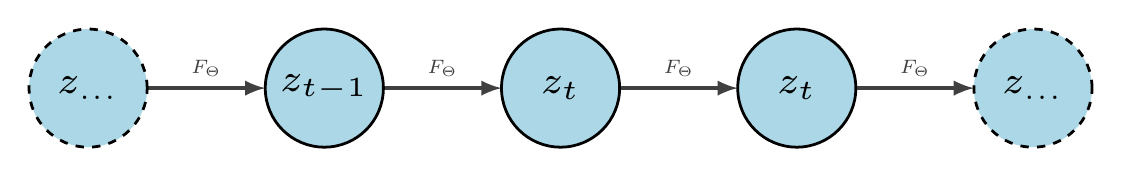
\begin{tikzpicture}
    \Vertex[x=0, style=dashed, size=1.5, label=$z_{...}$, fontscale=2.]{A}
    \Vertex[x=3,size=1.5, label=$z_{t-1}$, fontscale=2.]{B}
    \Vertex[x=6,size=1.5, label=$z_{t}$, fontscale=2.]{C}
    \Vertex[x=9,size=1.5, label=$z_{t}$, fontscale=2.]{D}
    \Vertex[x=12, style=dashed, size=1.5, label=$z_{...}$, fontscale=2.]{E}

    \Edge[label=$F_{\Theta}$,position=above, Direct](A)(B)
    \Edge[label=$F_{\Theta}$,position=above, Direct](B)(C)
    \Edge[label=$F_{\Theta}$,position=above, Direct](C)(D)
    \Edge[label=$F_{\Theta}$,position=above, Direct](D)(E)

  \end{tikzpicture}
  \caption[Basic computational graph]{\textbf{Basic computational graph}: The classical discrete dynamical system illustrated as an unfolded computational graph. Each node represents the state
  of the system at time $t$. The function $F_{\Theta}$ maps the state at time $t$ to the state at time $t+1$. The parameters $\Theta$ stay constant through time.}
  \label{fig:basic_graph}
\end{figure}

For a complete model we need to add external inputs to our graph representation and map the internal (hidden) states $z_{1 \cdots t}$ to outputs $\hat{x}_{1 \cdots t}$.
These outputs can then be used to compute the training loss $\mathcal{L}$ when compared to the target values $x_{1 \cdots t}$. 

The mapping from the latent space $\mathbb{R}^M$ to observation space $\mathbb{R}^N$ is called the observation equation or observation model.  

\begin{equation}
    \hat{x}_t = g(z_t)
\end{equation}
Note that $g: \mathbb{R}^M \rightarrow \mathbb{R}^N$ is not necessarily linear.

The loss function commonly used in this context is the mean squared error (MSE), which calculates the average squared difference between the
desired outputs $X=[x_1, \cdots, x_T]$  and the model outputs $\hat{X}=[\hat{x_1}, \cdots, \hat{x_T} ]$, with the possibility of 
incorporating an additional regularizing term.

\begin{equation}
    \mathcal{L} = \mathcal{L}_{MSE}(X, \hat{X}) + \mathcal{L}_{reg}(X, \hat{X}) = \frac{1}{T} \sum_{t=1}^{T}(x_i - \hat{x}_i)^2 + \mathcal{L}_{reg}(X, \hat{X})
    \label{eq:gen_loss}
\end{equation}


\begin{figure}
  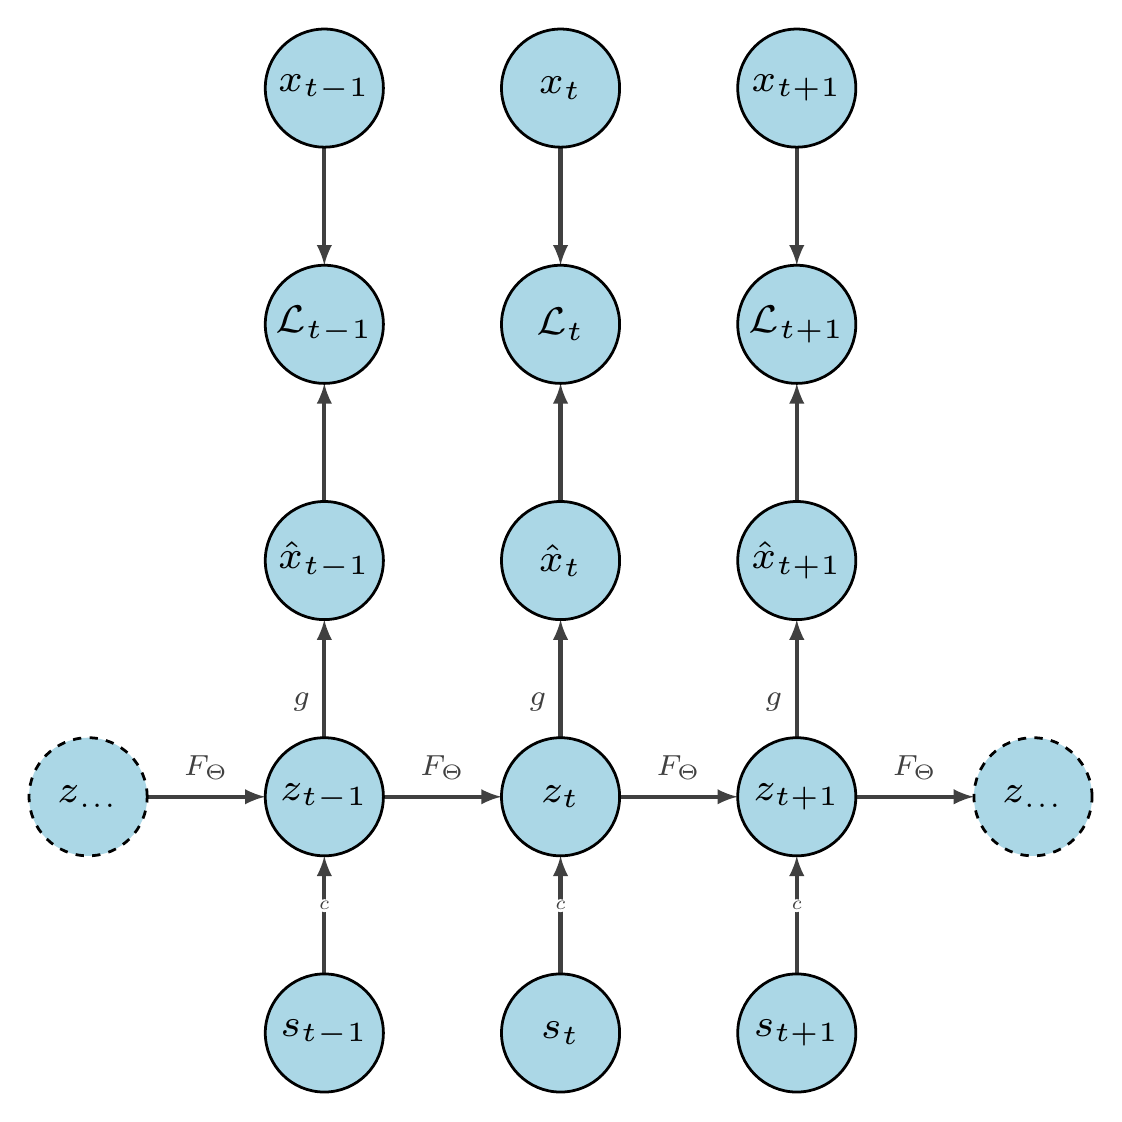
\begin{tikzpicture}
    \Vertex[x=0, style=dashed, size=1.5, label=$z_{...}$, fontscale=2.]{E0}

    \Vertex[x=3, y=-3, size=1.5, label=$s_{t-1}$, fontscale=2.]{A0}
    \Vertex[x=6, y=-3, size=1.5, label=$s_{t}$, fontscale=2.]{B0}
    \Vertex[x=9, y=-3, size=1.5, label=$s_{t+1}$, fontscale=2.]{C0}

    \Vertex[x=3, size=1.5, label=$z_{t-1}$, fontscale=2.]{A1}
    \Vertex[x=6, size=1.5, label=$z_{t}$, fontscale=2.]{B1}
    \Vertex[x=9, size=1.5, label=$z_{t+1}$, fontscale=2.]{C1}

    \Vertex[x=3, y=3, size=1.5, label=$\hat{x}_{t-1}$, fontscale=2.]{A2}
    \Vertex[x=6, y=3, size=1.5, label=$\hat{x}_{t}$, fontscale=2.]{B2}
    \Vertex[x=9, y=3, size=1.5, label=$\hat{x}_{t+1}$, fontscale=2.]{C2}

    \Vertex[x=3, y=6, size=1.5, label=$\mathcal{L}_{t-1}$, fontscale=2.]{A3}
    \Vertex[x=6, y=6, size=1.5, label=$\mathcal{L}_{t}$, fontscale=2.]{B3}
    \Vertex[x=9, y=6, size=1.5, label=$\mathcal{L}_{t+1}$, fontscale=2.]{C3}

    \Vertex[x=3, y=9, size=1.5, label=$x_{t-1}$, fontscale=2.]{A4}
    \Vertex[x=6, y=9, size=1.5, label=$x_{t}$, fontscale=2.]{B4}
    \Vertex[x=9, y=9, size=1.5, label=$x_{t+1}$, fontscale=2.]{C4}



    \Vertex[x=12, style=dashed, size=1.5, label=$z_{...}$, fontscale=2.]{E1}

    \Edge[label=$F_{\Theta}$,position=above, fontscale=1.5, Direct](E0)(A1)

    \Edge[label=$F_{\Theta}$,position=above, fontscale=1.5, Direct](A1)(B1)
    \Edge[label=$F_{\Theta}$,position=above, fontscale=1.5, Direct](B1)(C1)

    \Edge[label=$c$, position=above, Direct](A0)(A1)
    \Edge[label=$c$, position=above, Direct](B0)(B1)
    \Edge[label=$c$, position=above, Direct](C0)(C1)

    \Edge[label=$g$, position={below left=2mm}, fontscale=1.5, Direct](A1)(A2)
    \Edge[label=$g$, position={below left=2mm}, fontscale=1.5, Direct](B1)(B2)
    \Edge[label=$g$, position={below left=2mm}, fontscale=1.5, Direct](C1)(C2)

    \Edge[position=above, Direct](A2)(A3)
    \Edge[position=above, Direct](B2)(B3)
    \Edge[position=above, Direct](C2)(C3)

    \Edge[position=above, Direct](A4)(A3)
    \Edge[position=above, Direct](B4)(B3)
    \Edge[position=above, Direct](C4)(C3)


    \Edge[label=$F_{\Theta}$,position=above, fontscale=1.5, Direct](C1)(E1)
  \end{tikzpicture}

  \caption[Full graph of a recurrent neural network]{\textbf{Full graph of a recurrent neural network:} The RNN evolves forward in time from state $z_{t-1}$ to $z_{t}$ 
  with $F_{\Theta}$. Additional external inputs $s_{t}$ are added to the state $z_{t}$ via the function $c$.
  Observations $\hat{x}_t$ are produced from state $z_t$ by the observation function $g$. 
  The observations $\hat{x}_t$ and the ground truth $x_t$ are used to compute the loss $\mathcal{L}_t$.}
  \label{fig:full_graph}
\end{figure}

The full graph representation is shown in Figure \ref{fig:full_graph}. The RNN defined in Eq. \ref{eq:vanilla_rnn} and in Figure \ref{fig:full_graph} is universal in
the sense that it is Turing-complete \cite{chung2021turing}. More important for the applications in this work, they are proven to be dynamically universal, i.e. they are 
able to approximate any open dynamical system to an arbitrary accuracy \cite{schafer2006recurrent}. This approximation theorem for RNNs ensures the approximation capability
of RNNs, it does not give a way to find the model parameters for good approximations. Finding globally optimal parameters for neural networks is in general a 
NP-complete problem \cite{blum1988training}.


\section{Backpropagation through time}
Using the computational graph representation established in the previous section the computation of the gradient through an RNN is straightforward. One simply applies the 
general backpropagation algorithm known from feedforward neural networks to the unrolled computational graph. This algorithm is called backpropagation through time (BPTT)
and it can be used with any general-purpose gradient based methods to train the RNN.
Given the loss function from Eq. \ref{eq:gen_loss} we can use BPTT to compute the gradients with respect to each parameter $\theta_i \in \Theta$ by recursively applying the chain
rule backwards in time

\begin{equation}
    (\nabla \mathcal{L})_i = \frac{\partial \mathcal{L}}{\partial \theta_{i}} = \frac{1}{T} \sum_{t=1}^{T} \frac{\partial \mathcal{L}_{t}}{\partial \theta_{i}}
    = \frac{1}{T} \sum_{t=1}^{T} \sum_{k=1}^{t} \frac{\partial \mathcal{L}_{t}}{\partial \hat{x}_{t}} \frac{\partial \hat{x}_{t}}{z_{t}} \frac{\partial z_{t}}{\partial z_{k}} \frac{\partial z_{k}}{\partial \theta_{i}}
    \label{eq:bptt_grad}
\end{equation}

The term $\frac{\partial z_{t}}{\partial z_{k}}$ connects the latent state $z_{t}$ with the past latent state $z_{t-1}$. We can expand this term using the chain rule

\begin{equation}
    \frac{\partial z_{t}}{\partial z_{k}} = \frac{\partial z_{t}}{\partial z_{t-1}} \frac{\partial z_{t-1}}{\partial z_{k}} = \cdots 
    = \prod_{\tau=k}^{t-1} \frac{\partial z_{\tau+1}}{\partial z_{\tau}}
    \label{eq:Jacobian_product}
\end{equation}

This is a product of Jacobian matrices $J_{t} = \frac{\partial z_{t}}{\partial z_{t-1}}$ and is in each term of the inner sum in Eq. \ref{eq:bptt_grad}.


Computing the gradients of the loss function (Eq. \ref{eq:gen_loss}) with respect to the parameters is computationally expensive. 
This computation involves a forward pass, moving from left to right in the unrolled graph shown in Figure \ref{fig:bptt_graph}, 
followed by a backward pass moving from right to left through the entire graph once again.
Both the forward and backward passes are inherently sequential and cannot be parallelized since they depend on the previous hidden state.
Consequently, they possess a computational complexity of $\mathcal{O}(T)$ for an input sequence length of $T$. \newline 
Additionally, due to the necessity of storing the states computed during the forward pass for use in the backward pass, 
the memory cost of BPTT is also $\mathcal{O}(T)$.


\begin{figure}
  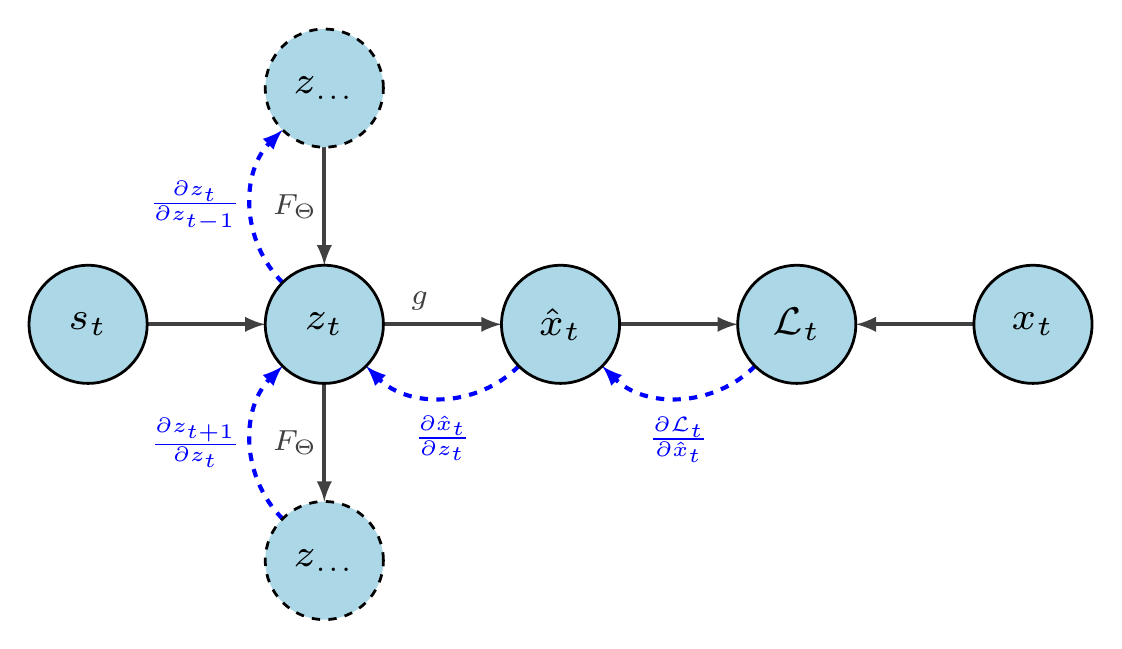
\begin{tikzpicture}

    \Vertex[y=3, style=dashed, size=1.5, label=$z_{...}$, fontscale=2.]{E0}
    \Vertex[y=0, x=-3, size=1.5, label=$s_{t}$, fontscale=2.]{A0}
    \Vertex[y=0, size=1.5, label=$z_{t}$, fontscale=2.]{A1}
    \Vertex[y=0, x=3, size=1.5, label=$\hat{x}_{t}$, fontscale=2.]{A2}
    \Vertex[y=0, x=6, size=1.5, label=$\mathcal{L}_{t}$, fontscale=2.]{A3}
    \Vertex[y=0, x=9, size=1.5, label=$x_{t}$, fontscale=2.]{A4}
    \Vertex[y=-3, style=dashed, size=1.5, label=$z_{...}$, fontscale=2.]{E1}

    \Edge[label=$F_{\Theta}$,position=left, fontscale=1.5, Direct](E0)(A1)
    \Edge[position=above, Direct](A0)(A1)
    \Edge[label=$g$, position={above left=2mm}, fontscale=1.5, Direct](A1)(A2)
    \Edge[position=above, Direct](A2)(A3)
    \Edge[position=above, Direct](A4)(A3)
    \Edge[label=$F_{\Theta}$,position=left, fontscale=1.5, Direct](A1)(E1)

    \Edge[label=$\frac{\partial \mathcal{L}_{t}}{\partial \hat{x}_{t}}$, position=below, fontscale=1.5, bend=45, style={dashed}, Direct, color=blue](A3)(A2)
    \Edge[label=$\frac{\partial \hat{x}_{t}}{\partial z_{t}}$, position=below, fontscale=1.5, bend=45, style={dashed}, Direct, color=blue](A2)(A1)
    \Edge[label=$\frac{\partial z_{t+1}}{\partial z_{t}}$, position=left, fontscale=1.5, bend=45, style={dashed}, Direct, color=blue](E1)(A1)
    \Edge[label=$\frac{\partial z_{t}}{\partial z_{t-1}}$, position=left, fontscale=1.5, bend=45, style={dashed}, Direct, color=blue](A1)(E0)


  \end{tikzpicture}

  \caption[Graph representation of BPTT]{\textbf{Graph representation of BPTT: } The RNN evolves forward (\textit{black}) in time with $F_{\Theta}$. 
  At time $t$ observations $\hat{x}_t$ are produced from state $z_t$ by the observation function $g$. The observations $\hat{x}_t$ and the ground truth $x_t$
  are compared in the loss $\mathcal{L}_t$.
  During the backwards pass (\textit{blue}) the graph is traversed in reverse. The partial derivatives are computed along the way.
  The Jacobians $J_t=\frac{\partial z_{t}}{\partial z_{t-1}}$ express the temporal dependency of states.}
  \label{fig:bptt_graph}
\end{figure}

\FloatBarrier
\section{Exploding and vanishing gradients} \label{sec:evg_problem}

Eq. \ref{eq:Jacobian_product} shows that gradients are propagated over long times if the sequence length $T$ becomes large. 
This can lead to them either vanishing or exploding, causing numerical issues during optimization. To illustrate the issue assume a
simple RNN of the form 

\begin{equation}
    z_{t} = \boldsymbol{W} z_{t-1}
    \label{eq:simple_rnn}
\end{equation}

where the weight matrix $W$ is diagonalizable with the decomposition $W = P D P^{-1}$, where $D$ is a diagonal matrix with the eigenvalues $\lambda_i$
of $W$ and $P$ is a nonsingular matrix consisting of the eigenvectors corresponding to the eigenvalues in $D$. The Jacobian is simply given by $J_t = W$ 
for all times $t$. Inserting this into Eq. \ref{eq:Jacobian_product} leads to the following

\begin{align}
    \frac{\partial z_{t}}{\partial z_{k}} = \prod_{\tau=k}^{t-1} J_{\tau+1}
                                          = \prod_{\tau=k}^{t-1} W 
                                          = \prod_{\tau=k}^{t-1} P D P^{-1}
                                          = P D^{t-k} P^{-1}
    \label{eq:bptt_evg}
\end{align}

We know from linear algebra that raising a diagonal matrix $D = \text{diag}(\lambda_i, \cdots, \lambda_M)$ to the power $n$ can be done by raising
the diagonal element to the power of $n$, so

\begin{equation}
    D^n = \text{diag}(\lambda_i^{n}, \cdots, \lambda_M^{n}).
    \label{eq:diag_power}
\end{equation}

From Eq. \ref{eq:diag_power} it is clear that the eigenvalues $|\lambda_i| < 0$ will decay towards 0 and the eigenvalues $|\lambda_i| > 0$ will diverge for large times. 
This phenomenon is called the exploding and vanishing gradient (EVG) problem and also occurs in more general RNNs. 

To give a general criterion for EVG, first define the spectral radius of a matrix $M \in \mathbb{R}^{M \times M}$ with eigenvalues $\lambda_1, \cdots, \lambda_M$ as 

\begin{equation}
    \rho (M) = \max \left( |\lambda_1|, \cdots, |\lambda_M| \right).
\end{equation}

Then the EVG criterion is given by 

\begin{equation}
    \left(\prod_{t=2}^{T} \rho(J_t)\right)^{\frac{1}{T-1}} = 
    \begin{cases}
        > 1 \rightarrow \text{exploding gradients} \\
        < 1 \rightarrow \text{vanishing gradients}
    \end{cases}
\end{equation}

The general case is not as easy to compute as in the simple case of \ref{eq:simple_rnn} as the Jacobians and their spectral radii change along the trajectory $z_{1:T}$.

It is important to note that the EVG problem cannot be avoided by simply constraining the parameter space to regions without EVGs. As shown in \cite{bengio1993problem},
whenever a model is able to represent long-term dependencies, the gradient of the long-term interaction has exponentially smaller magnitude than the gradient of 
short-term interactions. This means that the gradient signal can easily be hidden by small fluctuations arising from short-term dependencies.
In practice, experiments such as in \cite{bengio1994learning} have shown that when using stochastic gradient descent to train vanilla RNNs, 
the task of learning dependencies in sequences of only lengths 10 to 20 becomes progressively more challenging.

\section{Dealing with the exploding and vanishing gradient}

Since the EVG problem was discovered in the 90s, different attempts to solve the problem have been proposed. In the following I will only
give a brief overview, a more complete review of different methods can be found in \cite{pascanu2013difficulty}.

\subsection{\texorpdfstring{$L_1$}{ Lg} and \texorpdfstring{$L_2$}{ Lg} Regularization}

Assuming the recurrent weights are initialized such that $\rho(J)<1$, the $L_1$/$L_2$ regularizing terms can ensure that during training the eigenvalues
stay small, and thus the gradients can't explode. Regularization can however limit the model by preventing it to exhibit long term memory traces or learn
more complex attractor geometries in state space.

\subsection{Alternative architectures}
Alternative network architectures such as the long short-term memory (LSTM) net by \cite{hochreiter1997long} aim to eliminate the vanishing gradient problem by design. They rely on a special type of unit
with a self connection. The flow of information through a cell is regulated by learned input, output and forget gates. The design allows for gradients to
flow through the network unchanged and not vanish. This solution does not however prevent exploding gradients
and networks with these units are often harder to train as they have more dynamical variables and a higher number of parameters.

\subsection{Gradient Clipping}
Gradient clipping (GC) or rescaling is a common method to deal with exploding gradients by simply rescaling them if they go past a certain threshold to 
prevent a floating-point number overflow.

\begin{algorithm}
    \caption{Pseudocode for gradient clipping}\label{alg:cap}
    \begin{algorithmic}
        \State $\hat{g} \gets \frac{\partial \mathcal{L}}{\partial \Theta}$

        \If {$|\hat{g}| \geq \tau$}
            \State $\hat{g} \gets \frac{\text{threshold}}{\hat{g}}$
        \EndIf
    \end{algorithmic}
\end{algorithm}

Gradient clipping is simple and computationally efficient, but introduces the threshold value $\tau$ as another hyperparameter. In \cite{pascanu2013difficulty}
it suggested setting the threshold as the average norm of gradients $\langle|\frac{\partial \mathcal{L}}{\partial \Theta}|\rangle$ across large number
of updates multiplied by $\gamma \in [0.5, 10]$ such that $\tau = \gamma \langle|\frac{\partial \mathcal{L}}{\partial \Theta}| \rangle$. 

\subsection{Smart Initialization}
A further technique to deal with the EVG problem is to initialize the recurrent weights in such a way that they are easy to train and are good at modeling
long-range dependencies. This is the so-called initialization trick or smart initialization.

In \cite{le2015simple} it is proposed to use the ReLU activation function and initializing the hidden-to-hidden weight matrix $\boldsymbol{W}$ 
to the identity. This identity initialization has the property that error derivatives remain constant when backpropagated as long as no extra 
error-derivatives are added. This is similar to the behavior of the LSTMs forget gates which let error gradients pass with no decay. 

In \cite{talathi2015improving} it is proposed to initialize the hidden-to-hidden weight matrix $\boldsymbol{W}$ such that the maximum eigenvalue is 1 
and all others are smaller 1. This results in a line attractor configuration at initialization, meaning that the trajectory of the hidden states will 
evolve towards the principal axis with eigenvalue 1, thereby eliminating the conditions for exploding gradients. 

\section{Teacher Forcing}
Teacher forcing (TF) is a technique commonly used in training RNNs in a supervised learning setting. The name teacher forcing was coined by
\cite{williams1989learning}, who in turn cite \cite{jordan1986attractor} and \cite{pineda1988dynamics} for first introducing the method.
The idea is to replace or \textit{force} the hidden RNN state $z_i$ by a desired target state $d_i$ during training to guide the network towards the desired 
computational task. The desired target state is called teacher or forcing signal.

Next, let us define TF more formally. Let $F_{\Theta}$ be an RNN, $z_{t} \in \mathbb{R}^M$ the networks latent state and $d_t \in \mathbb{R}^M$ the desired 
target value. Define $I$ as the set of indices at which the network is forced. The state equation is given by

\begin{equation}
    z_{t+1} = \begin{cases}
        F_{\theta}(d_t) \text{ if } t \in I \\
        F_{\theta}(z_t) \text{ else }\\
    \end{cases}
    \label{eq:teacher_forcing}
\end{equation}

This form of teacher forcing forces the orbits of the RNN back on the ground truth orbits. It is important to note that in \cite{williams1989learning}, 
the observation equation is the identity function, i.e. $\hat{x}_t = z_t$, thus the forcing signal is simply set $d_t = x_t$ for all time steps $t \in I$. 

In order to retrieve useful error gradients, the loss function at forcing time $t$, $\mathcal{L}_t$, is computed prior to forcing,
so on the generated observation $\hat{x}_t$, not on the output of the forced network. At each forcing time step $t \in I$ the gradients are truncated.
To see this, evaluate the Jacobian $J_{t+1}$

\begin{equation}
    J_{t+1} = \frac{\partial z_{z+1}}{\partial z_{t}} = \frac{\partial F_{\Theta (d_t)}}{\partial d_t} \frac{\partial d_t}{\partial z_t} = \frac{\partial F_{\Theta (d_t)}}{\partial d_t} \cdot 0 = 0.
\end{equation}

The term $\frac{\partial d_t}{\partial z_t} = 0$ because the forcing signal $d_t$ does not depend on the hidden state $z_t$. This means that TF circumvents
the EVG problem but also has a limited capability to learn long term dependencies because the gradients are cut off at the forcing time steps $t \in I$.

In \textit{sparse} teacher forcing, the forcing signal is only applied sparsely at time intervals $\tau$. This of course introduces another hyperparameter
into training. In \cite{NEURIPS2022_495e55f3} it is argued that the forcing interval should be chosen in accordance to the maximal Lyapunov exponent
$\lambda_{max}$ of the system, which gives us a predictability time $\tau = \frac{\ln2}{\lambda_{max}}$. Given a time interval $\tau$ chosen for a 
time series of length $T$ we can then define the set of forcing indices

\begin{equation}
    I = \{ t | t = k \tau < T, k \in \mathbb{N} \}
\end{equation}

In this sparse approach the model is allowed to diverge from the true dynamics in the short term to learn the observed dynamics but is regularly forced 
back to the true behavior, cutting the gradients and avoiding EVG. But this is only true in the simplest case that the latent and observation space are
of equal dimension $N=M$. In the more common case that $z_t \in \mathbb{R}^M$ and $x_t \in \mathbb{R}^N$ with $N<M$ forcing can be applied to the $N$ 
"visible units" of the state while the $M-N$ other hidden units are unchanged. The risk of EVG remains as gradients can still flow through these 
hidden units.

In \cite{doya1992bifurcations} a different form of teacher forcing, the so-called \textit{weak} teacher forcing is introduced. Instead of replacing 
the entire hidden state at certain time steps as in \ref{eq:teacher_forcing}, the is generated state variable $z_t$ and the desired target $d_t$ are 
linearly interpolated using a weighting coefficient $\alpha \in [0,1]$.

\begin{equation}
    z_{t+1} = F_{\Theta}((1-\alpha)z_z + \alpha d_t)
    \label{eq:weak_tf}
\end{equation}

In \cite{doya1992bifurcations} it is hypothesized that the solutions found by this weak forcing regime are more likely to be stable than those found 
in the fully forced case. We can once again compute the Jacobian in the weak TF case

\begin{equation}
    J_{t+1} = \frac{\partial z_{z+1}}{\partial z_{t}} = \frac{\partial F_{\Theta} (\tilde{z_t})}{\partial \tilde{z_t}} \frac{\partial \tilde{z_t}}{\partial z_t} = (1-\alpha) F_{\Theta}'(\tilde{z_t})
\end{equation}

with $\tilde{z_t} = (1-\alpha) z_t + \alpha d_t$. It follows that the chain of Jacobians remains intact, hence EVG may still occur in weak TF and the 
hyperparameter $\alpha$ is introduced.

\section{Piecewise Linear Recurrent Neural Network (PLRNN)}

In this thesis I will use the so called piecewise linear recurrent neural network (PLRNN) architecture first introduced in \cite{durstewitz2017state}.
The state equation of the PLRNN is 

\begin{equation}
    z_{t} = \boldsymbol{A} z_{t-1} + \boldsymbol{W} \Phi (z_{t-1}) + \boldsymbol{C} s_{t-1} + h.
    \label{eq:plrnn}
\end{equation}
where $z_t \in \mathbb{R}^M$ is latent state vector at time $t$, $\Phi$ is the ReLU activation function, $\boldsymbol{W}$ is an off-diagonal
matrix of connection weights and $\boldsymbol{A}$ a diagonal matrix holding the autoregressive weights.

This model formulation is motivated by neuroscience. From this point of view, the entries of the latent state $z_{i_t}$ can be interpreted as membrane
potential, the diagonal elements in $\boldsymbol{A}$ are seen as the neurons individual membrane time constants and the off-diagonal elements in 
$\boldsymbol{W}$ represent synaptic connections between neurons. The ReLU activation models the fact that neurons only show spiking activities
above a certain firing threshold. From a mathematical point of view, Eq. \ref{eq:plrnn}  has the form of an autoregressive model with a nonlinear
basis expansion in the latent variables $z_{i_t}$. 

A particular advantage of the PLRNN model is that many of its dynamical properties can be computed analytically while simultaneously enjoying the same universal 
approximation capabilities of the vanilla RNN. For example, setting external inputs to $0$, fixed points $z_{\ast}$ can be obtained analytically 
by solving $2^M$ linear equations. 

\begin{equation}
    z_{\ast} = (A + W - \mathbb{1})^{-1} 
\end{equation}

Besides fixed points, $k-cycles$ (including their stability) (\cite{koppe2019identifying}, \cite{schmidt2019identifying}, \cite{brenner2022tractable})
and Jacobians of the system can be computed, which in turn also allows for computation of the Lyapunov spectrum (\cite{mikhaeil2022difficulty}).

\section{PLRNN extensions}

\cite{brenner2022tractable} extended the basic PLRNN structure by adding a linear spline basis expansion, called the dendritic PLRNN (dendPLRNN), to increase the expressivity
of each unit and improve performance, especially for low dimensional systems. The state equation is given by 

\begin{equation}
    z_t = \boldsymbol{A} z_{t-1} + \boldsymbol{W} \sum_{b=1}^{B} \alpha_b \phi(z_{t-1} - h_b) + h_0
    \label{eq:dendPLRNN}
\end{equation}

with slope-threshold pairs $\{ \alpha_b, h_b \}_{b=1}^B$, where $B$ is the number of bases. It can be shown that the dendPLRNN can be reformulated as a higher dimensional
conventional PLRNN, so the properties of PLRNN are preserved.

However, in this thesis I will use the shallow PLRNN (shPLRNN), a "one hidden layer" PLRNN architecture. The state equation is 

\begin{equation}
    z_{t} = \boldsymbol{A} z_{t-1} + \boldsymbol{W_1} \phi \left( \boldsymbol{W}_2 z_{t-1} + h_2 \right) + h_1
    \label{eq:shPLRNN}
\end{equation}
with latent states $z_t \in \mathbb{R}^M$ and the diagonal matrix $\boldsymbol{A} \in \mathbb{R}^{M \times M}$ as in Eq. \ref{eq:plrnn}. 
$\boldsymbol{W}_1 \in \mathbb{R}^{M \times L}$ and $\boldsymbol{W}_2 \in \mathbb{R}^{L \times M}$ are rectangular connectivity matrices, 
$h_2 \in \mathbb{R}^L$ and $h_1 \in \mathbb{R}^M$ are thresholds. Dimensions $L > M$ are used. 

By expanding each unit's activation into a weighted sum of ReLU nonlinearities, this formulation appears similar to the dendPLRNN. \cite{hess2023generalized} show that it is 
indeed possible to rewrite the shPLRNN into a dendPLRNN. Again this implies that the desired mathematical properties of the PLRNN model are preserved.

Both the dendPLRNN and the shPLRNN can be equipped with a clipping mechanism that prevents states from diverging to $\infty$ due to unbounded ReLU nonlinearities.
For shPLRNN this clipping is given by

\begin{equation}
    z_{t} = \boldsymbol{A} z_{t-1} + \boldsymbol{W_1} \left[\phi \left( \boldsymbol{W}_2 z_{t-1} + h_2 \right) - \phi \left( \boldsymbol{W}_2 z_{t-1}\right) \right]+ h_1 
    \label{eq:clippedShPLRNN}
\end{equation}

This mechanism guarantees bounded orbits provided the eigenvalues of $\boldsymbol{A}$ are smaller than 1.

\section{Linear Observation model}

To map the latent states to observation space the PLRNN is typically equipped with an affine observation equation

\begin{equation}
    \hat{x}_t = \boldsymbol{B} z_t + b
    \label{eq:obs_eq_basic}
\end{equation}

with weights $\boldsymbol{B} \in \mathbb{R}^{N \times M}$ and a bias $b \in \mathbb{R}^N$. The bias term is typically dropped when dealing with preprocessed time series data
which has been standardized, as is the case in this work. Hence, equation \ref{eq:obs_eq_basic} simplifies to a linear observation equation.

\section{Identity Teacher Forcing}

The simplest case of the linear observation equation is an identity mapping between a subspace of the latent states $z_t \in \mathbb{R}^M$ and the outputs of the model 
$\hat{x}_t \in \mathbb{R}^N$. This achieved by setting $B$ to a fixed matrix $\mathcal{I} \in \mathbb{R}^{N \times M}$, which maps the first $N$ units of $z_t$ directly 
on to $x_t$. $\mathcal{I}$ can be defined as 

\begin{equation}
    \mathcal{I}_{ij} = \begin{cases}
        1, & \text{ if } i=j \text{ and } i,j \leq N \\
        0, & \text{ else }
    \end{cases}
\end{equation}

This implies splitting $z_t$ into hidden and observation or readout units 

\begin{equation}
    z_t = \begin{bmatrix}
        z_t^{obs} = \hat{x}_t \\
        z_t^{hid}
    \end{bmatrix} = \begin{bmatrix}
        z_t^1 = \hat{x}_t^1 \\ 
        \vdots \\
        z_t^N = \hat{x}_t^N \\
        \vdots \\
        z_t^M
    \end{bmatrix}
\end{equation}

such that 

\begin{equation}
    \hat{x}_t = \mathcal{I}z_t.
    \label{eq:ident_obs}
\end{equation}

This allows for \textit{direct teacher forcing} to be applied by simply supplying the teacher signal directly to the observation neurons $z_t^{obs}$. The forcing signal 
does not change the hidden units $z_t^{hid}$. This gives us 
\begin{equation}
    d_t = \begin{bmatrix}
        x_t \\
        z_t^{hid}
    \end{bmatrix}
    \label{eq:indent_tf}
\end{equation}

as the desired target value $d_t$ which is applied in different TF variants (see Eq. \ref{eq:teacher_forcing} and Eq. \ref{eq:weak_tf}).
Note that this makes training susceptible to the EVG problem regardless or forcing protocol because gradients can flow freely without truncation through the space of hidden
neurons $z^{hid}$.

\section{Inversion Teacher Forcing}

To allow for more expressivity in the observation model, we do not want to constrain the $B \in \mathbb{R}^{N \times M}$ matrix. In this case we can no longer map the observations
back to the latent state to obtain the target values $d_t$ we need as forcing signals. In \cite{mikhaeil2022difficulty} a TF method is introduced for this case which 
I will refer to as \textit{Inversion Teacher Forcing}. The inversion of the linear out mapping is approximated using the psuedo-inverse $B^{+}$ 
(also known as the Moore-Penrose inverse) of $B$. Hence, the desired target values $d_t$ are computed as follows:

\begin{equation}
    d_t = B^{+}x_t = (B^{T}B)^{-1}B^T x_t
    \label{eq:inversion_tf}
\end{equation}

In this case the full latent state vector $z_t$ is replaced by the target values $d_t$, which means gradient are truncated in the case of sparse TF. In the paper 
\cite{mikhaeil2022difficulty} itself, sparse TF is used and the forcing interval is estimated using the maximal Lyapunov exponent $\lambda_{max}$ of the system.

\begin{equation}
    \tau = \frac{\ln 2}{\lambda_{max}}
\end{equation}

Now that I have introduced the PLRNN and its implementation with the linear observation model, it's time to adapt this existing framework to model fMRI time series and 
define a new observation model.

\section{BOLD observation model} \label{sec:bold_obs}

The aim of this thesis is to expand the existing PLRNN training framework to fMRI data. For this I will next briefly introduce the physical basics behind fMRI recordings 
and how to the model the "BOLD" response.

\subsection{Physical principals of fMRI}

The term \textit{functional magnetic resonance imaging} (fMRI) generally refers to the imaging of brain activation detectable by changes in regional cerebral blood flow.

To support the cells of the brain with oxygen ($O_2$), it is transported within the red blood cells bound in hemoglobin molecules. When hemoglobin molecules bind to $O_2$, they 
form oxyhemoglobin (OHb), which has no unpaired electrons and is weakly diamagnetic. When oxygen is released, deoxyhemoglobin (DHb) is left with 4 unpaired electrons
exposed at each iron center, causing it to become strongly paramagnetic. The presence of paramagnetic deoxyhemoglobin within the blood cells creates local magnetic field 
distortions. These distortions cause regional $T2$ and $T2^*$ relaxations times to decrease and suppress the MR signal.
These Signal intensity variations in the MR image are called the \textit{blood oxygen level dependent} (BOLD) contrast. Functional MRI is a temporally resolved sequence of
$T2^*$ weighted MR images.

During cerebral activation, regional cerebral blood flow (CBF) increases, but the cerebral metabolic rate of oxygen consumption (CMR$O_2$) is not proportionally elevated.
CBF and CMR$O_2$ are thus said to be "uncoupled" (\cite{fox2012coupling}). Instead, more freshly oxygenated blood is supplied to active regions of the brain than is required
for its immediate metabolic needs. This is means that the relative concentration of DHb in activated areas will decrease, local field inhomogenities diminish and the 
BOLD signal in activated areas increases.

\subsection{Modelling the Hemodynamic Response}

The BOLD signal has been shown to have a consistent response to a short stimulus, peaking after around 6 seconds and then falling back to baseline over the next several 
seconds. For the purposes of estimating the BOLD signal in an experimental paradigm, the SPM framework (\cite{penny2011statistical}) makes use of a canonical 
hemodynamic response function (HRF). This function is assumed to be the response of the system (as reflected by the MR signal) to a brief,
intense period of neural stimulation. The canonical HRF in SPM is defined as the difference of two Gamma function, see Eq. \ref{eq:canonical_hrf}. 
The implementation, including the shape parameters, was ported from the SPM MATLAB implementation into julia for this thesis. 

\begin{equation}
    h(t) = A \left(\frac{t^{\alpha_1 - 1} \beta^{\alpha_1} e^{-\beta_1 t}}{\Gamma (\alpha_1)} - c \frac{t^{\alpha_2 -1} \beta^{\alpha_2} e^{-\beta_2 t}}{\Gamma (\alpha_2) } \right)
    \label{eq:canonical_hrf}
\end{equation}

The shape parameters are already estimated by the SPM implementation, only the repetition or repeat time (RT) parameter is passed to the hrf function. 
It is the temporal resolution at which the fMRI time series was acquired. In the following I will refer to an $hrf$
function with a given RT as $hrf_{RT}$ for clarity. $hrf$ functions with varying repetition times are shown in figure \ref{fig:hrf_comp}.

\begin{figure}
    \includegraphics[width=\textwidth]{Images/hrf_comp.png}
    \caption[Comparison of $hrf$ functions with varying repetition times]
    {\textbf{Comparison of $hrf$ functions with varying repetition times}}
    \label{fig:hrf_comp}
\end{figure}

The observed BOLD signal $x[t]$ is assumed to be driven by underlying neural event signal $s[t]$. 
A convolution with the $hrf$ function and added measurement noise $\epsilon[t]$ is used to model the relationship between the BOLD response and the 
underlying neural event. The BOLD signal in a given voxel (or region of interest) at time $t$, $x[t]$, is thus given by the following equation:

\begin{align}
    x[t] &= \sum_{\tau=1}^{M} h[\tau] s(t-\tau) + \epsilon[t] & \epsilon[t] \sim \mathcal{N}(0, \Sigma)
\end{align}

where $\epsilon[t] \sim \mathcal{N}(0, \Sigma)$ is a Gaussian white noise term with diagonal covariance matrix $\Sigma = diag(\sigma_{11}^2, \cdots, \sigma_{NN}^2)$.
The convolution operation will be covered in more depth in section \ref{sec:conv}.

\subsection{Defining the BOLD observation equation} \label{sec:bold_obs_eq}

An appealing feature of the state space model framework is that different measurement modalities can be accommodated by connecting different observation
models to the same latent model. To model fMRI time series we therefore simply need to adapt the observation equation \ref{eq:obs_eq_basic} to the BOLD response 
model in equation \ref{eq:canonical_hrf}. The latent states $z_t$ of the PLRNN with its universal approximation capabilities should then learn to model the
(unknown/unobservable) neural activity when trained on fMRI time series. 

The modified observation equation is as follows

\begin{equation}
    \hat{x}_t = \boldsymbol{B} \left( (hrf \ast z)_t\right) + \boldsymbol{J}r_t + \epsilon_t
    \label{eq:bold_obs_eq}
\end{equation}

where $\hat{x}_t \in \mathbb{R}^N$ is the estimated BOLD signal in $N$ voxels at time $t$ generated from the latent states $z \in \mathbb{R}^M$ convolved with the $hrf$ function.
The convoluted latent states are observed through a linear-Gaussian model and additional nuisance predictors $r_t \in \mathbb{R}^n$, which account for movement artifacts, 
are added. $\boldsymbol{J} \in \mathbb{R}^{N \times P}$ is the coefficient matrix of these nuisance variables.

This observation equation however introduces a major complication. The observations in Eq. \ref{eq:bold_obs_eq} do not just depend on the current state $z_t$ as in the 
simple linear model, but on a set of states $z_{\tau:t}$ across several previous time steps due to the convolution operation. It is now no longer clear how to calculate the 
forcing signal because the model outputs $\hat{x}_t$ depend on multiple latent states, therefore the target value $d_t$ for the latent state $z_t$ cannot simply
be calculated from one data point $x_t$ anymore.

To solve this problem I will introduce the mathematical frameworks of the Fourier and the Wavelet Transformation in the next two chapters.
These will give us the mathematical tools needed to handle convolution and \textit{deconvolution}, the inverse operation to convolution.
 % Background Theory 


\chapter{Fourier Transform} \lhead{\emph{Fourier Transformation}}

The Fourier transform is a mathematical operation that decomposes a function or signal into its constituent frequencies.
In this chapter I will give a short overview of the Fourier transform (FT) and properties important to this work. A precise
mathematical approach including the proofs of the properties given here can be found in \cite{serov2017fourier}, more applied information
focused on discrete FT and signal processing can be found in \cite{smith1997scientist} and \cite{puthusserypady2021applied}.

\section{Continuous Fourier Transform}

\begin{definition}[Continuous Fourier Transform]
    For a function $f \in L^1(\mathbb{R}^d)$ the Fourier transform $\mathscr{F}$ is defined as 

    \begin{equation}
        \mathscr{F} \{ f(x) \}(k) = \widehat{f}(k) = \int_{\mathbb{R}^d} f(x) e^{-i k^T x} d^d x
    \end{equation}
    \label{def:fourier_trafo}
\end{definition}

the output of the transform is a complex-valued function of frequency. The term Fourier transform refers to both this complex-valued function $\widehat{f}$ 
and the mathematical operation $\mathscr{F}$.

In the following I will list some important properties of the Fourier transform. First I will define two operators that will clear up notation.

\begin{definition}
    The translation operator $\tau_y$ is defined for $y \in \mathbb{R}^d$ as $\tau_y f = f(y + \cdot)$.
    The dilatation operator $\sigma_A$ is defined for $A \in \mathbb{R}^{d \times d}$ as $\sigma_A f = f(A \cdot)$.
\end{definition}

\begin{proposition}[Properties of the Fourier transform]
    For $f, g \in L^1(\mathbb{R}^d)$ the following properties hold

    \begin{enumerate}

        \item Linearity: For $a, b \in \mathbb{C}$
        \begin{align*}
            \mathscr{F} \{ a \cdot f(x) + b \cdot g(x) \} = a \cdot \mathscr{F} \{f(x)\} + b \cdot \mathscr{F} \{ g(x) \}
        \end{align*}

        \item Translation: For $y \in \mathbb{R}^d$
        \begin{align*}
            \widehat{(\tau_y f)}(k) = e^{i y^T k} \widehat{f}(k)
        \end{align*}

        \item Modulation: For $a \in \mathbb{R}$
        \begin{align*}
            \mathscr{F} \{e^{-i a x} f(x) \} = \widehat{\tau_a f}
        \end{align*}

        \item Time scaling: For $A \in \mathbb{R}^{d \times d}$ an invertable matrix
        \begin{align*}
            \widehat{\sigma_A f}(k) = \frac{\widehat{f}(A^{-T} k)}{\| \det A \|}
        \end{align*}
        Note that in one dimension $d = 1$ this formula simplifies to $\widehat{\sigma_a f}(k) = \frac{1}{|a|} \widehat{f}(\frac{k}{a})$ with $a \in \mathbb{R}$.

        \item Inverse Fourier Transform: 
        \begin{align*}
            f(x) = \mathscr{F}^{-1} \{ \widehat{f}(k) \}(x) := \frac{1}{(2\pi)^d} \int_{\mathbb{R}^d} \widehat{f}(k) e^{i x^T k} dk 
        \end{align*}
    \end{enumerate}
    \label{prop:fourier_properties}
\end{proposition}

\section{Discrete Fourier Transform}
The discrete Fourier transform (DFT) is the discrete version of the Fourier transform. It transforms a signal represented as a discrete sequence into its equivalent 
representation in the frequency domain.

\begin{definition}[Discrete Fourier Transform]
    Given a signal $\{x[n] \}$ of length $N \in \mathbb{N}$ with $x[n] \in \mathbb{C} \quad \forall n \in [\![0, N]\!]$. 
    The discrete Fourier Transform $\mathscr{F}$ is defined as 
    \begin{equation}
        \mathscr{F}\{x[n]\}[k] = \widehat{x}[k] = \sum_{n=0}^{N-1} x[n] e^{-\frac{2\pi i}{N} kn}
    \end{equation}
    \label{eq:dft}
\end{definition}

Linearity, modulation and translation properties also hold for the DFT, given the arguments are integer valued and remain in the definition space.
The inverse discrete Fourier transform(IDFT) also exists and is defined as follows:

\begin{definition}[Inverse Discrete Fourier Transform]
    Given a complex valued signal $\{ \widehat{x}[k] \}$ of length $N \in \mathbb{N}$ with $\widehat{x}[k] \in \mathbb{C} \quad \forall k \in [\![0, N]\!]$.
    The inverse discrete Fourier Transform $\mathscr{F}^{-1}$ is defined as 
    \begin{equation}
        \mathscr{F}^{-1}\{ \widehat{x}[k] \}[n] = x[n] = \frac{1}{N} \sum_{k=0}^{N-1} \widehat{x}[k] e^{\frac{2\pi i}{N}kn}
    \end{equation}
\end{definition}

It holds that $x[n] = \mathscr{F}^{-1} \{\mathscr{F} \{x[n]\}\}$ and $\widehat{x}[k]= \mathscr{F}^{-1} \{\mathscr{F} \{\widehat{x}[k]\}\}$

\subsection{Unitary DFT}\label{sec:unitary_dft}

Another way of representing the DFT is as a matrix transform. If we represent out signal as vector $X =  \begin{bmatrix}x[1], \cdots, x[N] \end{bmatrix}^T$,
the DFT can be expressed as the DFT matrix

\begin{equation}
    W = \frac{1}{\sqrt{N}}
    \begin{bmatrix}
        1 & 1 & 1 & 1 & \cdots & 1 \\
        1 & \omega & \omega^2 & \omega^3 & \cdots & \omega^{N-1} \\
        1 & \omega^2 & \omega^4 & \omega^6 & \cdots & \omega^{2(N-1)} \\
        1 & \omega^3 & \omega^6 & \omega^9 & \cdots & \omega^{3(N-1)} \\
        \vdots & \vdots & \vdots & \ddots & \ddots \\
        1 & \omega^{N-1} & \omega^{2(N-1)} & \omega^{3(N-1)} & \cdots & \omega^{(N-1)(N-1)} \\
    \end{bmatrix}
    \label{eq:dft_matrix}
\end{equation}

with $\omega = e^{-\frac{2 \pi i}{N}}$. The inverse transform has the same matrix structure but with opposite-sign exponents. 
Please also note that in this matrix representation the normalization factor $\frac{1}{\sqrt{N}}$ is present for both forward and transform.
The placing of the normalization factor and the sign are just convention and differ across the literature.

This choice however makes the DFT matrix $W$ and its inverse $W^{-1}=W^{\ast}$ unitary. This allows us to interpret the DFT simply as basis transformation of the signal
into the Fourier basis. It also follows immediately that the DFT conserves the energy of the signal. This is formalized in the following theorem.

\begin{theorem}[Plancherel theorem]
    Given two complex valued signals $\{x[n]\}$, $\{y[n]\}$ of length $N \in \mathbb{N}$ and their Fourier transforms $\{\widehat{x}[n]\}$, $\{\widehat{y}[n]\}$, 
    the following equality holds:

    \begin{equation}
        \sum_{n=0}^{N-1} x[n] y^*[n] = \sum_{k=0}^{N-1} \widehat{x}[k] \widehat{y}^*[k]
    \end{equation}

    In the special case of $\{x[n]\} = \{y[n]\}$ for all $n$, we get $\sum_{n=0}^{N-1} | x[n] |^2 = \sum_{k=0}^{N-1} | \widehat{x}[k] |^2$.
    This result can also be extended to the continuous case. For $f, g \in L^1(\mathbb{R}^d) \cap L^2(\mathbb{R}^d)$ it holds that

    \begin{equation}
        \int_{\mathbb{R}^d} f(x) g^*(x) d^dx = \int_{\mathbb{R}^d} \widehat{f}(k) \widehat{g}^*(k) d^d k
    \end{equation}
    again in the case that $f=g$ this simplifies to energy conservation $\int_{\mathbb{R}^d} |f(x)|^2 d^dx = \int_{\mathbb{R}^d} |\widehat{f}(k)|^2 d^d k$
    \label{th:plancherel}
\end{theorem}

\section{Fast Fourier Transform}

The naive computation of the DFT \ref{eq:dft} is very computationally expensive. It requires $N^2$ complex multiplications and $N^2-N$ complex additions, 
giving the algorithm a complexity of $\mathcal{O}(N^2)$. By exploiting the symmetry ($e^{\frac{2 \pi i}{N}(k+N/2)} = - e^{\frac{2 \pi i}{N} k}$) and 
the periodicity ($e^{\frac{2 \pi i}{N}(k+N)} = e^{\frac{2 \pi i}{N} k}$) of the phase factor a more efficient algorithm can be derived.

\subsection{Cooley–Tukey FFT algorithm}

The Cooley-Turkey FFT algorithm is the most common FFT algorithm. It reexpresses the DFT of a signal of composite length $N = N_1 N_2$ as $N_1$ DFTs of size $N_2$. This is 
applied recursively to reduce the computational complexity to $\mathcal{O}(N \log(N))$ for highly composite numbers. Subsequently, I will outline the
fundamental concept behind the algorithm.

Assume we have a signal $\{ x[n] \}$ of length $N$ where $N$ is not prime and can be written as the product of two integers $N = LM$. Note that this assumption is not restrictive 
since the signal can be padded with zeros to ensure the condition is met. 

First the sequence is stored as a two-dimensional array indexed by the row index $l \in [\![0, L-1]\!]$ and the column index $m \in [\![0, M-1]\!]$. Choose the mapping $n = M l + m$
to map the index $n$ to the indices $(l,m)$. The computed DFT values can be mapped in a similar fashion by mapping the index $k$ to the pair $(p,q)$ with $k = Mp +q$.

Now suppose the signal is mapped as $x[l,m]$ and the results as $\widehat{x}[p,q]$. Then the DFT equation \ref{eq:dft} can be written as double sum of the array elements

\begin{equation}
    \widehat{x}[p,q] = \sum_{m=0}^{M-1}\sum_{l=0}^{L-1} x[l, m] e^{\frac{2 \pi i}{N}(Mp + q)(mL + l)}
    \label{eq:fft_double_sum}
\end{equation}

Now we can use the following identities of the phase factor: $e^{\frac{2 \pi i }{N}mqL} = e^{\frac{2 \pi i }{N/L}mq} = e^{\frac{2 \pi i }{M}mq} $, 
$e^{\frac{2 \pi i }{N}Mpl} = e^{\frac{2 \pi i }{N/M}pl} = e^{\frac{2 \pi i }{L}pl}$, $e^{\frac{2 \pi i }{N}Nmp} = 1$.
With these identities, equation \ref{eq:fft_double_sum} can be written as 

\begin{equation}
    \widehat{x}[p, q] = \sum_{l=0}^{L-1} \left\{ e^{\frac{2 \pi i }{N}lq} \left[  \sum_{m=0}^{M-1}x[l, m] e^{\frac{2 \pi i }{M}mq} \right] \right\} e^{\frac{2 \pi i }{L}lp}
\end{equation}

This expression now involves the computation of DFTs of length $M$ and $L$. The number of complex multiplications have been reduced from $N^2$ to $N(M+L+1)$ and the number of complex
additions from $N(N-1)$ to $N(M+L+2)$. When $N$ is a highly composite number, i.e. N can be factored into a product of prime numbers

\begin{equation}
    N = r_1 r_2 \dots r_{\nu}
    \label{eq:n_composite_number}
\end{equation}

then the decomposition can be repeated $\nu - 1$ more times, reducing the computational complexity each time. 

In the special case of $r_1 = r_2 = \dots = r_{\nu} = 2$, so that $N = 2^{\nu}$ the computation of the $N$-point DFT has a regular pattern. The number $r$ is called the \textit{radix}
of the FFT algorithm. For $r=2$ the resulting FFT algorithm is termed the radix-2 FFT algorithm.

Consider the case of signal length $N=2^{\nu}$. Select $M=N/2$ and $L=2$. This selection results in splitting the signal into two subsignals $f_1[n]$ and $f_2[n]$ corresponding 
to the even even-numbered and odd-numbered samples of $\{x[n] \}$.

\begin{align*}
    f_1[n] &= x[2n] & n \in [\![0, N/2-1]\!] \\
    f_2[n] &= x[2n + 1]
\end{align*}

Now the DFT can be expressed in terms of DFTs of the decimated sequences as follows:

\begin{equation}
    \widehat{x}[k] = \sum_{m=0}^{N/2-1}x[2m] e^{\frac{2 \pi i}{N}2mk} + \sum_{m = 0}^{N/2-1} x[2m + 1] e^{\frac{2 \pi i }{N}(2m+1)k}
\end{equation}

using $e^{\frac{2 \pi i }{N}2} = e^{\frac{2 \pi i}{N/2}}$ we can rewrite this to

\begin{align}
    \widehat{x}[k] &= \sum_{m=0}^{N/2-1}f_1[m] e^{\frac{2 \pi i}{N/2}mk} + \sum_{m=0}^{N/2-1}f_2[m] e^{\frac{2 \pi i}{N/2}mk} \\
                   &= \widehat{f_1}[k] + e^{\frac{2 \pi i }{N}k} \widehat{f_2}[k] & k \in [\![0, N-1]\!] \label{eq:fft_radix_decomp}
\end{align}

where $\widehat{f_1}[k]$ and $\widehat{f_2}[k]$ are the $N/2$ DFTs of $f_1[k]$ and $f_2[k]$. Using the fact that $\widehat{f_1}[k]$ and $\widehat{f_2}[k]$ are periodic with 
period $N/2$. In addition, $e^{\frac{2 \pi i}{N}(k+N/2)} = - e^{\frac{2 \pi i}{N}k}$. Hence, we can rewrite \ref{eq:fft_radix_decomp} as 

\begin{align}
    \widehat{x}[k] &= \widehat{f_1}[k] + e^{\frac{2 \pi i}{N}k} \widehat{f_2}[k] \nonumber\\
    \widehat{x}[k + \frac{N}{2}] &= \widehat{f_1}[k] - e^{\frac{2 \pi i}{N}k} \widehat{f_2}[k] \label{eq:fft_butterfly}
\end{align}

\begin{figure}

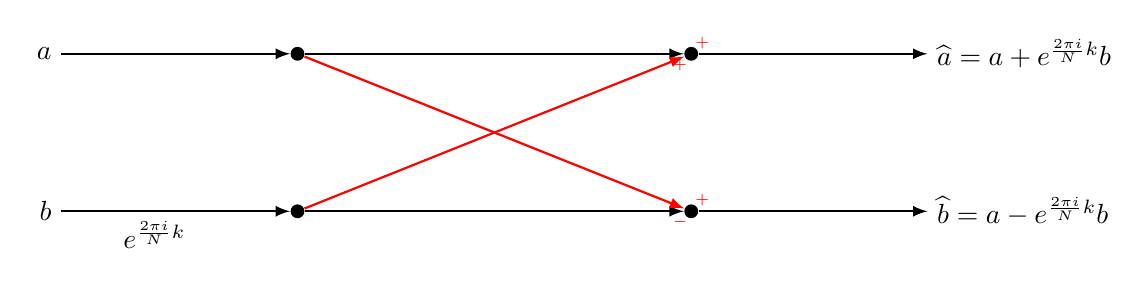
\begin{tikzpicture}[y=-1cm]

\node (A0) at (0, 0) [left]{$a$};
\node (B0) at (0, 2) [left]{$b$};

\node[circle,fill=black,minimum size=5pt,inner sep=0pt] (A1) at (3, 0) {};
\node[circle,fill=black,minimum size=5pt,inner sep=0pt] (B1) at (3, 2) {};

\draw[-latex,thick] (A0) -- (A1);
\draw[-latex,thick] (B0) -- (B1);

\node (B0) at (1.7, 2.3) [left]{$e^{\frac{2 \pi i}{N}k}$};


\node[circle,fill=black,minimum size=5pt,inner sep=0pt] (A2) at (8, 0) {};
\node[circle,fill=black,minimum size=5pt,inner sep=0pt] (B2) at (8, 2) {};

\draw[-latex,thick] (A1) -- (A2);
\draw[-latex,thick] (B1) -- (B2);

\draw[-latex,thick,red] (A1) -- (B2);
\draw[-latex,thick,red] (B1) -- (A2);

\node[red] at (A2) [shift={(315:0.2)}] {\tiny$+$};
\node[red] at (A2) [shift={(135:0.2)}] {\tiny$+$};
\node[red] at (B2) [shift={(315:0.2)}] {\tiny$+$};
\node[red] at (B2) [shift={(135:0.2)}] {\tiny$-$};

\node (A3) at (11, 0) [right]{$\widehat{a}=a + e^{\frac{2 \pi i}{N}k} b$};
\node (B3) at (11, 2) [right]{$\widehat{b}=a - e^{\frac{2 \pi i}{N}k} b$};

\draw[-latex,thick] (A2) -- (A3);
\draw[-latex,thick] (B2) -- (B3);

\end{tikzpicture}

\caption{Basic butterfly diagram in the decimation-in-time FFT algorithm}
\label{fig:butterfly_basic}
\end{figure}

The basic computation in \ref{eq:fft_butterfly} is called the \textit{butterfly} structure because the flow graph resembles a butterfly as shown in Figure \ref{fig:butterfly_basic}.
It is the basic computation performed in the radix-2 FFT. It can be seen that by this process the number of complex multiplications has been reduced from $N^2$ to $N^2/2+N/2$. We can repeat this process, the so-called 
\textit{decimation-in-time}, recursively for both $f_1[n]$ and $f_2[n]$. For $N=2^{\nu}$, this decimation can be performed $\nu$ times reducing the number of multiplications to 
$\frac{N}{2}\log_2 N$ and the number of additions to $N \log_2 N$.

For illustration, Figure \ref{fig:butterfly_fft} depicts the computation of an $N=8$-point DFT. In three stages, first 4 two-point DFTs are computed, then 2 four-point DFTS and 
lastly one 8-point DFT. These smaller DFTs are combined in a butterfly structure to form the larger DFT.

\begin{figure}

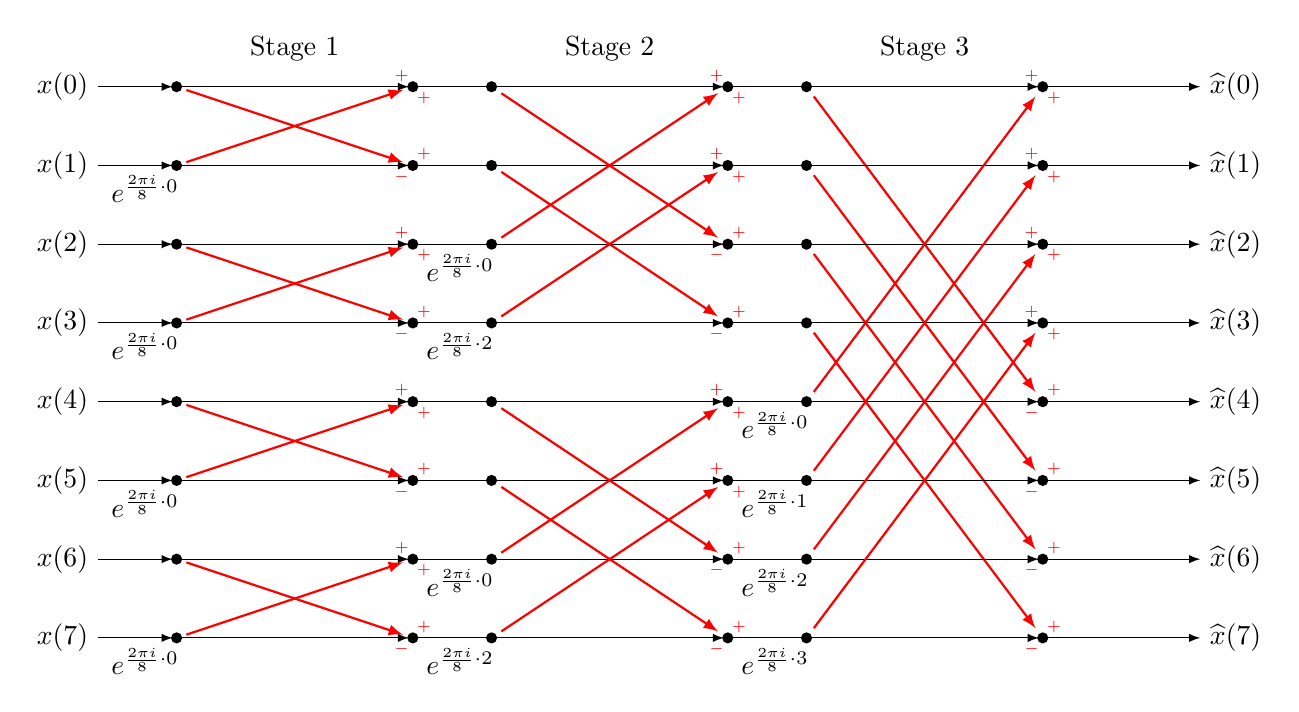
\begin{tikzpicture}[y=-1cm]

\node (t1) at (1.5, -0.2) [above]{Stage 1};
\node (t2) at (5.5, -0.2) [above]{Stage 2};
\node (t3) at (9.5, -0.2) [above]{Stage 3};


\foreach\y in {0,...,7} 
{
  \pgfmathtruncatemacro\yy{mod(abs(3.5-\y)+0.5,2)==0?\y:(\y<4?\y+3:\y-3)} % F value
  \draw[-latex] (-1,\y) node [left] {$x(\y)$} -- (-0.05,\y);
  \draw[-latex] (12,\y) -- (13,\y) node [right] {$\widehat{x}(\y)$};
  \foreach\x in {0,1,2}
  {
    \draw[-latex] (4*\x,\y) --++ (2.95,0) ;
    \draw(4*\x+3,\y) --++ (1,0);
    \foreach\z in {0,3}
      \node[circle,fill,inner sep=0.5mm] at (4*\x+\z,\y) {};
    \pgfmathtruncatemacro\i{pow(2,\x)}
    \pgfmathtruncatemacro\j{\i-2*\i*mod(div(\y,\i),2)} % delta y for the arrows
    \node (A) at (4*\x,\y)      {};
    \node (B) at (4*\x+3,\y+\j) {};
    \draw[-latex,thick,red] (A) -- (B);
    \ifnum\j < 0
      \node[red] at (B) [shift={(225:0.2)}] {\tiny$+$};
      \node[red] at (B) [shift={ (45:0.2)}] {\tiny$+$};
    \else
      \pgfmathtruncatemacro\k{mod(\y,\i)*(2-abs(\x-1))} % W exponent
      \node[red] at (B) [shift={(315:0.2)}] {\tiny$+$};
      \node[red] at (B) [shift={(135:0.2)}] {\tiny$-$};
      \node at (4*\x-0.8, \y+\j) [shift={(0.4,0.3)}] {$e^{\frac{2 \pi i}{8}\cdot \k}$};
    \fi
  }
}
\end{tikzpicture}
\caption{Visualization of a 3 stage radix-2 FFT algorithm}
\label{fig:butterfly_fft}
\end{figure}

Implementing the FFT efficiently poses further challenges that I will not cover here. In this work I will use the FFTW library, implementation and design details
can be found in \cite{FFTW.jl-2005}.



\section{Convolution and the Convolutional Theorem}\label{sec:conv}

Having established the basic properties of the Fourier transform, I will now introduce the convolution operation and its important properties.

\begin{definition}[Convolution]
    Let $f, g \in L^1(\mathbb{R}^d)$ be integrable functions. The convolution of $f$ and $g$, written as $(f \ast g)$, is defined as
    \begin{equation}
        (f \ast g)(t) := \int_{\mathbb{R^d}} f(\tau) g(t - \tau) d^d \tau
    \end{equation}
    \label{eq:conv_def}
\end{definition}
The convolution operation is also defined for discrete functions.

\begin{definition}[Discrete Convolution]
    Let $f, g$ be complex-valued functions defined on $\mathbb{Z}$. The convolution of $f$ and $g$ is defined as
    \begin{equation}
        (f \ast g)[n] := \sum_{m=-\infty}^{\infty} f[m] g[n - m]
        \label{eq:disc_conv}
    \end{equation}
    Note that in the case that $g$ is non-zero only on a finite interval $[\![-M, M]\!]$ the series in the above definition can be replaced with a finite summation 
    \begin{equation}
        (f \ast g)[n] = \sum_{m=-M}^{M} f[m] g[n - m].
        \label{eq:disc_conv_finite}
    \end{equation}
\end{definition}

The definition of the discrete convolution in Eq. \ref{eq:disc_conv_finite} can be rewritten as a matrix vector multiplication. Write the signal as a vector
$x = [ x[1], \cdots, x[N] ]^{T}$. The convolution with the impulse response $h = [h[1], \cdots, h[M]]^T$ is given by the multiplication with the 
$(M+N-1) \times N$ convolution matrix

\begin{equation}
    y = h \ast x = 
    \begin{bmatrix}
        h[1] & 0 & \cdots & 0 & 0 \\
        h[2] & h[1] & \cdots & 0 & 0 \\
        h[3] & h[2] & \cdots & 0 & 0 \\
        \vdots & h[3] & \cdots & h[1] & 0 \\
        h[m-1] & \vdots & \ddots & h[2] & h[1] \\
        h[m] & h[m-1] &    & \vdots & h[2] \\
        0 & h[m] & \ddots & h[m-2] & \vdots \\
        0 & 0 & \cdots & h[m-1] & h[m-2] \\
        \vdots & \vdots &    & h[m] & h[m-1] \\
        0 & 0 & \cdots & 0 & h[m] 
    \end{bmatrix}
    \begin{bmatrix}
        x[1] \\
        x[2] \\
        x[3] \\
        \vdots \\
        x[N]
    \end{bmatrix}
    \label{eq:conv_matrix}
\end{equation}

This depiction of convolution as matrix transformation is useful as an alternative mathematical perspective on the convolution operation, and it 
was used in the implementation part of this work as calculating the loss gradient over matrix multiplication is already built into the Julia Flux
framework.

\begin{proposition}[Properties of the Convolution operation]
    The following properties hold in both the continuous and the discrete case. For either 
    $f, g, h \in L^1(\mathbb{R}^d)$ or $f, g, h$ complex-valued functions on $\mathbb{Z}$.  

    \begin{enumerate}
            \item Commutativity
                \begin{align*}
                    f \ast g = g \ast f
                \end{align*}
            \item Associativity
                \begin{align*}
                    f \ast (g \ast h) = (f \ast g) \ast h
                \end{align*}
            \item Distributivity
                \begin{align*}
                    f \ast (g + h) = (f \ast g) + (f \ast h)
                \end{align*}
            \item Associativity with scalar multiplication: For $a \in \mathbb{C}$
                \begin{align*}
                    a (f \ast g) = (a f) \ast g
                \end{align*}
            \item Identity: Convolution with the delta distribution $\delta$ is simply the identity operation
                \begin{align*}
                    f \ast \delta = f
                \end{align*}
    \end{enumerate}
    \label{prop:conv_properties}
\end{proposition}

Convolution and the Fourier transform are connected by the following convolutional theorem, which states that the Fourier transform translates 
the convolution operation in the time domain to a simple multiplication in the frequency domain.

\begin{theorem}[Convolutional Theorem]
    Let $f, g \in L^1(\mathbb{R^d})$ be integrable functions on $\mathbb{R^d}$ with Fourier transforms $F=\mathscr{F}\{f\}$ and $G=\mathscr{F}\{g\}$.
    Define their convolution $h = f \ast h$ and its Fourier transform $H = \mathscr{F} \{ f \ast h \}$. The convolutional theorem states that

    \begin{equation}
        H(k) = F(k) \cdot G(k)
    \end{equation}
    where $\cdot$ denotes pointwise multiplication.

    Applying the inverse FT $\mathscr{F}^{-1}$ immediately gives us the corollary
    \begin{equation}
        h(x) = \mathscr{F}^{-1} \{ F \cdot G \}(x).
    \end{equation}

    The convolutional theorem also holds in the discrete case where $f, g$ complex-valued signals and $\mathscr{F}$ denotes the DFT and $\mathscr{F}^{-1}$
    the IDFT.
    \label{th:conv_theorem}
\end{theorem}

The convolutional theorem allows us to efficiently compute convolutions. Note that both the definition in Eq. \ref{eq:disc_conv_finite} and the matrix
multiplication in Eq. \ref{eq:conv_matrix} require $N^2$ operations for $N$ output values. Using the convolutional theorem and the FFT algorithm
the computational complexity can be reduced to $\mathcal{O}(N \log N)$.

If we recall the depiction of the DFT as a unitary transformation in section \ref{sec:unitary_dft} and the convolution matrix in Eq. \ref{eq:conv_matrix}, 
it follows from the convolutional theorem that the DFT diagonalizes convolutional matrices. The Fourier basis is the eigenbasis of the convolution
operation.

\section{Deconvolution}

Deconvolution is the inverse operation to convolution. Given the functions $g$ and $h$, the objective of deconvolution is to find $f$ given the 
convolution equation 

\begin{equation}
    f \ast g = h.
    \label{eq:conv_eq}
\end{equation}

In the simple case of \ref{eq:conv_eq} we can simply use the convolutional theorem \ref{th:conv_theorem} to solve the equation in Fourier space.

\begin{align}
    F(k) G(k) &= H(k) \\
    F(k) &= \frac{H(k)}{G(k)} \\
    f(x) &= \mathscr{F}^{-1}\left(\frac{H}{G}\right)(x) \label{eq:inverse_filtering}
\end{align}

In practice, we however do not have the ideal case shown in \ref{eq:conv_eq}. Usually, $h$ is a recorded signal of a physical system and $f$
is the signal we wish to recover, but that has been convolved by a \textit{filter} or \textit{impulse response} $g$ when measuring the signal.
In real measured systems we typically have a measurement error term that has to be added to \ref{eq:conv_eq}, resulting in 

\begin{equation}
    (f \ast g) + \epsilon = h
    \label{eq:conv_real} 
\end{equation}

In this case $\epsilon$ is the noise term added to our recorded signal. Using the \textit{inverse filtering} approach in Eq. \ref{eq:inverse_filtering}
is now no longer correct. In fact, the signal-noise-ratio is typically worsened and high frequency terms are erroneously amplified. The problems
of deconvolution have long been known in the physics community, a discussion can be found in \cite{jones1970problem}.

\subsection{Wiener Deconvolution} \label{sec:Wiener_deconv}

To address the issues of the simple inverse filtering approach, the so-called Wiener Deconvolution was introduced in \cite{wiener1964extrapolation}. 
This approach again is applied in the frequency domain and attempts to minimize the impact of deconvolved noise at frequencies which have a poor
signal-to-noise ratio.

Given a system as in Eq. \ref{eq:conv_real}, the Wiener deconvolution attempts to provide filter $k$ to estimate $f$ as follows

\begin{equation}
    \hat{f}(t) = (k \ast h)(t)
\end{equation}

where $\hat{f}(t)$ is an estimate of $f(t)$ that minimizes the mean squared error (MSE). The Wiener deconvolution filter is naturally written in 
the Fourier domain as 

\begin{equation}
    K(k) = \frac{G^*(k) S(k)}{|G(k)|^2 S(k) + N(k)}
    \label{eq:wiener_deconv}
\end{equation}

where 

\begin{itemize}
    \item $K(k)$ and $G(k)$ are the Fourier transforms of $k(t)$ and $g(t)$
    \item $S(k) = \mathbb{E}[|F(k)|^2]$ is the mean power spectral density of the original signal $f(t)$
    \item $N(k) = \mathbb{E}[|\mathcal{E}(k)|^2]$ is the mean power spectral density of the noise $\epsilon(t)$
    \item the superscript $^*$ denotes complex conjugation.
\end{itemize}

The filtering operation can then be immediately carried out in the Fourier domain:

\begin{equation}
    \hat{F}(k) = K(k) H(k)
    \label{eq:wiener_filter_fourier}
\end{equation}

Applying the inverse Fourier transform then gives us the estimate of the original signal

\begin{equation}
    \hat{f}(t) = \mathscr{F}^{-1}(\hat{F})(t)
\end{equation}

An important limitation of this approach is that estimates of the exact impulse response of the system
and the mean power spectral density (PSD) of both the noise and the original, unknown signal are needed to perform the deconvolution. In the case of BOLD
time series the impulse response is known, it is the hemodynamic response function. The PSDs of the underlying signal and the noise are however not known.
In the next section on wavelets I will introduce the mathematical tools needed to obtain estimates of the original signal and the noise. 
These will allow us to apply Wiener deconvolution to BOLD time series.


\chapter{Wavelet Transformation} \lhead{\emph{Wavelet Transformation}}


This chapter provides a comprehensive overview of both the continuous and discrete wavelet transforms. Firstly, I will define Wavelets and 
showcase the mathematical theory behind the continuous wavelet transform (CWT). From there I will cover the discrete wavelet transform (DWT) 
and the fast wavelet transform, which allows for efficient computation of the DWT. With all that mathematical machinery in place I will then 
discuss how to use the wavelet transformation for noise estimation and denoising in a simple and effective manner.

I will note here that definitions and notations of wavelet theory are not consistent across literature. 
This issue is compiled by the fact that authors also use different definitions for the Fourier transform 
(i.e. different placing of the normalization factor), which underlies much of the wavelet theory. I followed \cite{sauer-notes},
\cite{mallat2008wavelet} and \cite{shah2022wavelet} for the definitions and theorems presented in this chapter but I did have to adapt them in part to be consistent. 

\section{Continuous Wavelet Transformation}
The fundamental idea behind the wavelet transformation is to analyze through the scale. Wavelets are used in the wavelet transformation the same way sin and cos are used
in the Fourier transformation. In the Fourier transformation, a function is transformed to a new basis given by sin and cos functions in frequency space.
Note that the sin and cos functions do not appear in the definition of FT introduced earlier because we only used the $e^{ikx}$. These functions 
are connected with the identity $e^{ikx} = cos(kx) + i \sin(kx)$.

The basis functions of the Fourier transform are localized in the frequency domain, each sin/cos has a single frequency, but not in the time domain,
where they are periodic and non-vanishing. This means that for periodic,
continuous signals the Fourier transform only needs a small amount of coefficients to obtain a good approximation of the signal.
In addition, noise limited to certain frequencies can be easily detected and filtered. 

Local signals containing discontinuities, on the other hand, cannot be approximated easily and one needs a large amount of Fourier coefficients to approximate them well.
Furthermore, localized time information is stored in the phase of the Fourier transformation, so modifications to the signals in frequency space
e.g. filtering may corrupt transient time information, leading to unwanted side effects.

These problems are addressed by wavelet transformations. Wavelets are, just like sin and cos in the Fourier transformation, used as basis functions
to represent a signal in the frequency domain. The major difference is that wavelets are localized in time and frequency domain. 
Therefore, wavelets are well-suited to approximate data containing sharp discontinuities. 
Another advantage of wavelets is that their width in time and frequency can vary.
This way one has long low frequency basis functions for frequency analysis and short basis functions to isolate discontinuities. The idea is illustrated
in figure \ref{fig:wavelet_trafo_sketch}.

\begin{figure}
    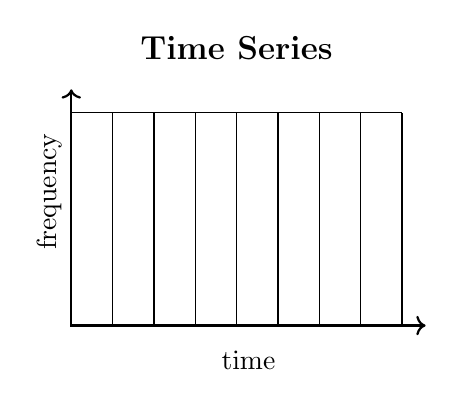
\begin{tikzpicture}[scale=1.5]
        % Draw axes
        \draw [<->,thick] (0,2) node (yaxis) [above] {}
            |- (3,0) node (xaxis) [right] {};

        \node[below=0.2cm] at (1.5, 0) {time};
        \node[rotate=90,above=0.2cm] at (0, 1) {frequency};
        \draw (2.8,0) coordinate (e_1) -- (2.8,1.8) coordinate (e_2);
        \draw (0,1.8) coordinate (e_3) -- (2.8,1.8) coordinate (e_2);

        \foreach \x in {0,...,8}
           {
                \draw (0.35*\x, 0) coordinate (vs_\x) -- (0.35*\x, 1.8) coordinate (ve_\x);
           }

        \node[above,font=\large\bfseries] at (current bounding box.north) {Time Series};
    \end{tikzpicture}%
\qquad
    \hspace{1cm}
    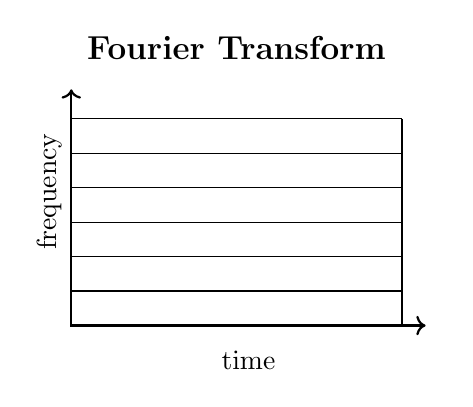
\begin{tikzpicture}[scale=1.5]
        % Draw axes
        \draw [<->,thick] (0,2) node (yaxis) [above] {}
            |- (3,0) node (xaxis) [right] {};

        \node[below=0.2cm] at (1.5, 0) {time};
        \node[rotate=90,above=0.2cm] at (0, 1) {frequency};
        \draw (2.8,0) coordinate (e_1) -- (2.8,1.75) coordinate (e_2);

        \foreach \y in {0,...,6}
           {
                \draw (0, 0.292*\y) coordinate (hs_\y) -- (2.8, 0.292*\y) coordinate (he_\y);
           }
            
        \node[above,font=\large\bfseries] at (current bounding box.north) {Fourier Transform};
    \end{tikzpicture}

    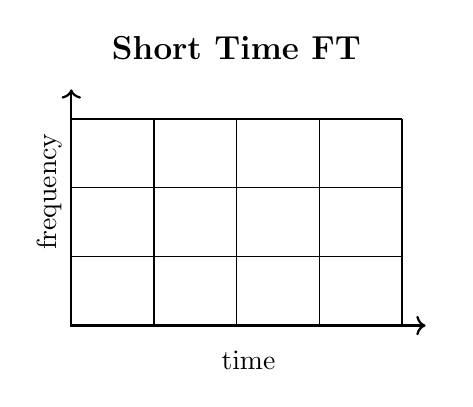
\begin{tikzpicture}[scale=1.5]
        % Draw axes
        \draw [<->,thick] (0,2) node (yaxis) [above] {}
            |- (3,0) node (xaxis) [right] {};

        \node[below=0.2cm] at (1.5, 0) {time};
        \node[rotate=90,above=0.2cm] at (0, 1) {frequency};
        \draw (2.8,0) coordinate (e_1) -- (2.8,1.75) coordinate (e_2);

        \foreach \y in {0,...,3}
           {
                \draw (0, 0.583*\y) coordinate (hs_\y) -- (2.8, 0.583*\y) coordinate (he_\y);
           }

           \foreach \x in {0,...,4}
           {
                \draw (0.7*\x, 0) coordinate (vs_\x) -- (0.7*\x, 1.75) coordinate (ve_\x);
           }
            
        \node[above,font=\large\bfseries] at (current bounding box.north) {Short Time FT};
    \end{tikzpicture}
    \qquad
    \hspace{1cm}
    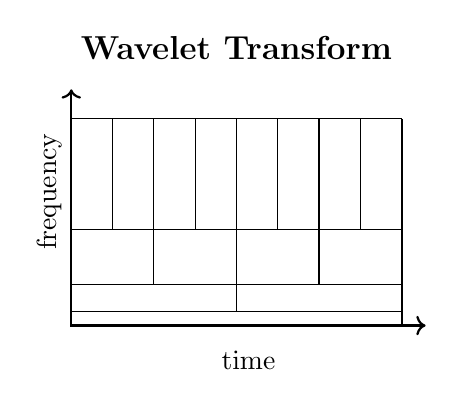
\begin{tikzpicture}[scale=1.5]
        % Draw axes
        \draw [<->,thick] (0,2) node (yaxis) [above] {}
            |- (3,0) node (xaxis) [right] {};

        \node[below=0.2cm] at (1.5, 0) {time};
        \node[rotate=90,above=0.2cm] at (0, 1) {frequency};
        \draw (2.8,0) coordinate (e_1) -- (2.8,1.75) coordinate (e_2);

        %horizontal lines
        \draw (0, 0.33*0.35) coordinate (hs_1) -- (2.8, 0.33*0.35) coordinate (he_1);
        \draw (0, 0.35) coordinate (hs_2) -- (2.8, 0.35) coordinate (he_2);
        \draw (0, 2.33*0.35) coordinate (hs_3) -- (2.8, 2.33*0.35) coordinate (he_3);
        \draw (0, 5*0.35) coordinate (hs_4) -- (2.8, 5*0.35) coordinate (he_4);

        %vertical lines
        \draw (0.466*3, 0.33*0.35) coordinate (vs_1) -- (0.466*3, 1.75) coordinate (ve_1);

        \draw (0.466*1.5, 0.35) coordinate (vs_21) -- (0.466*1.5, 1.75) coordinate (ve_21);
        \draw (0.466*4.5, 0.35) coordinate (vs_22) -- (0.466*4.5, 1.75) coordinate (ve_22);

        \draw (0.466*0.75, 2.33*0.35) coordinate (vs_31) -- (0.466*0.75, 1.75) coordinate (ve_31);
        \draw (0.466*2.25, 2.33*0.35) coordinate (vs_32) -- (0.466*2.25, 1.75) coordinate (ve_32);
        \draw (0.466*3.75, 2.33*0.35) coordinate (vs_33) -- (0.466*3.75, 1.75) coordinate (ve_33);
        \draw (0.466*5.25, 2.33*0.35) coordinate (vs_34) -- (0.466*5.25, 1.75) coordinate (ve_34);

        \node[above,font=\large\bfseries] at (current bounding box.north) {Wavelet Transform};
    \end{tikzpicture}
    \caption[Schematic overview of time/frequency resolution of different transformations]{A schematic overview of the time and 
    frequency resolutions of the different transformations in comparison with the original time-series dataset. 
    The size and orientation of the blocks indicate how small the features are that we can distinguish in the time and frequency domain.}
    \label{fig:wavelet_trafo_sketch}
\end{figure}

For a more mathematically precise formulation, let us first define a Wavelet

\begin{definition}[Wavelet]
    A function $\psi \in L^{2}(\mathbb{R})$ is called a Wavelet if it satisfies the following conditions

    \begin{enumerate}
        \item mean free $\int_{\mathbb{R}} \psi (t) dt = 0$
        \item normalized $\|\psi \|_2 = \sqrt{\int_{\mathbb{R}} \psi(t) \psi^{\ast}(t) dt} = 1$
        \end{enumerate}%
        In many cases an additional condition is required:
        \begin{enumerate}[resume*]
        \item admissibility $\int_{\mathbb{R}} \frac{\hat{\psi}(\omega) \hat{\psi}^{\ast}(\omega)}{|\omega|} d\omega < \infty$
    \end{enumerate}
    \label{def:wavelet}
\end{definition}

A function $\psi$ satisfying the definition is called the \textit{mother-wavelet}. From this \textit{mother-wavelet} we can generate a family of functions, the so-called 
\textit{Daughter-Wavelets}, as follows

\begin{equation}
    \Psi = \left\{ \psi_{a, b}(t) = \frac{1}{\sqrt{a}} \psi \left( \frac{t - b}{a} \right) | a \in (0, \infty), b \in \mathbb{R} \right\}
\end{equation}

Note that $\psi \in L^2(\mathbb{R})$ implies $\psi_{a, b} \in L^2(\mathbb{R})$. Furthermore, the normalization is preserved

\begin{equation}
    \| \psi_{a, b} \|^2_2 = \frac{1}{a} \int_{\mathbb{R}} \left| \psi \left(\frac{t - b}{a}\right) \right|^2 = \int_{\mathbb{R}} | \psi (u) |^2 du = \|\psi \|^2_2
\end{equation}

and the Fourier transform of the \textit{daughter-wavelet} $\psi_{a, b} \in L^2(\mathbb{R})$ is given by

\begin{align}
    \hat{\psi}_{a, b}(w) &= \int_{\mathbb{R}} \frac{1}{\sqrt{a}} \psi \left( \frac{t-b}{a}\right) e^{-i \omega t} dt \nonumber \\
                         &= \sqrt{a} e^{i b \omega} \int_{\mathbb{R}} \psi(\tau) e^{-i a \omega \tau} d \tau \nonumber \\
                         &= \sqrt{a} e^{i b \omega} \hat{\psi}(a \omega)
\end{align}

The parameter $a$ is the scaling parameter, which measures the degree of compression or scale, and $b$ is the translation parameter, measuring the time location of the wavelet.

Using these definitions, we can formally define the wavelet transform as follows: 
\begin{definition}[Continuous wavelet transform]
    Let $\psi$ be a Wavelet as defined in \ref{def:wavelet} and $f \in L_2(\mathbb{R})$. The wavelet transform of $f$ is defined as 
    \begin{equation}
        \mathscr{W}_{\psi}\{f\}(a,b) = \int_{\mathbb{R}}f(t)\frac{1}{\sqrt{a}} \psi^{\ast} \left( \frac{t - b}{a} \right) dt
        \label{eq:def_cwt}
    \end{equation}
    where * is the complex conjugate, $a \in (0, \infty)$ and $b \in \mathbb{R}$.
    \label{def:cwt}
\end{definition}

In the following proposition I have compiled some fundamental properties of the wavelet transform.
\begin{proposition}[Properties of the wavelet transform]
    Let $\alpha, \beta \in \mathbb{C}, \delta \in \mathbb{R}, \gamma > 0$ be scalars, $\psi, \phi$ admissible wavelets and $f, g \in L^2(\mathbb{R})$. Then the following
    properties hold

    \begin{enumerate}
        \item Linearity $\mathscr{W}_{\psi} \{\alpha f + \beta g\}(a,b) = \alpha \mathscr{W}_{\psi} \{f\}(a,b) + \beta \mathscr{W}_{\psi} \{g\}(a,b)$
        \item Translation $\mathscr{W}_{\psi}\{\tau_{\delta} f \}(a,b) = \mathscr{W}_{\psi}\{f\}(a, b+\delta)$
        \item Dilation $\mathscr{W}_{\psi} \{\sigma_{\gamma} f \}(a,b) = \mathscr{W}_{\psi}\{f\}(\frac{a}{\gamma}, \frac{b}{\gamma})$
        \item Symmetry $\mathscr{W}_{\psi}\{f\}(a,b) = \mathscr{W}_{f}\{\psi\}^{\ast}(\frac{1}{a}, \frac{b}{a})$
        \item Parity $\mathscr{W}_{P \psi} \{Pf\}(a,b) = \mathscr{W}_{\psi}(a, -b)$
        \item Anti-linearity $\mathscr{W}_{\alpha \psi + \beta \phi}\{f\}(a,b) = \alpha^{\ast} \mathscr{W}_{\psi} \{f\} (a,b) + \beta^{\ast} \mathscr{W}_{\phi}\{f\}(a,b)$
        \item Translation in wavelet: $\mathscr{W}_{\tau_{\delta} \psi}\{f\}(a,b) = \mathscr{W}_{\psi}\{f\}(a,b- a \delta)$
        \item Dilation in wavelet: $\mathscr{W}_{\sigma_{\gamma} \psi} \{f\}(a,b) = \mathscr{W}_{\psi}(\gamma a, b)$.
    \end{enumerate}
\end{proposition}

Some important notes on the definition \ref{def:cwt}

\begin{enumerate}
    \item The definition reminds us of the definition of the Fourier transform \ref{def:fourier_trafo}. The kernel $\psi_{a, b}$ plays the same role as the kernel $e^{ikx}$
          in the FT. The kernel of the wavelet transform is however a two-parameter family of functions determining the scale and location of the wavelet.
    
    \item Both the Fourier transform and the wavelet transform are linear transformations. But unlike the Fourier transform, the wavelet transform is not a single transform,
          but a group of transforms determined by the underlying wavelet.

    \item For a fixed scale $a$, the wavelet transform $\mathscr{W}_{\psi}\{f\}(a,b)$, as a function of $b$, represents the detail information contained in the signal
          $f$ at scale $a$.
    
    \item If the mother wavelet $\psi(t)$ posses $n$-vanishing moments, we can use the Taylor expansion of $f$ at $a=b$ and insert it in \ref{eq:def_cwt}
    
    \begin{multline}
        \mathscr{W}_{\psi}\{f\}(a,b) = f(b) \int_{\mathbb{R}} \psi_{a, 0}^{\ast}(t-b) dt + f^{(1)}(b)\int_{\mathbb{R}}(t-b) \psi_{a, 0}^{\ast}(t-b) + \\
        \frac{f^{(2)}(b)}{2} \int_{\mathbb{R}}(t-b)^2 \psi_{a, 0}^{\ast}(t-b) + \cdots + \frac{f^{(n)}(b)}{n!} \int_{\mathbb{R}}(t-b)^n \psi_{a, 0}^{\ast}(t-b) + \cdots
        \label{eq:cwt_tayler_exp}
    \end{multline}

    It follows that the first $n$ terms of \ref{eq:cwt_tayler_exp} vanish and do not contribute to $\mathscr{W}_{\psi}\{f\}(a,b)$.

    \item We can rewrite the wavelet transform using the Fourier transform.
    \begin{equation}
        \mathscr{W}_{\psi}\{f\}(a,b) = \sqrt{a} \int_{\mathbb{R}} \hat{f}(k) \hat{\psi}^{\ast}(a k) e^{ibk} dk.
        \label{eq:cwt_with_ft}
    \end{equation}

    \item We can Fourier transform the wavelet transform $\mathscr{W}_{\psi}\{f\}(a,b)$ as a function of $b$ using the equation \ref{eq:cwt_with_ft} above
    \begin{equation}
        \mathscr{F} \left\{ \mathscr{W}_{\psi}\{f\}(a,b)\right\}(k) = \sqrt{a} \hat{f}(k) \hat{\psi}^{\ast}(ak)
        \label{eq:ft_of_cwt}
    \end{equation}
\end{enumerate}

Before continuing we need another important definition that relates two wavelets to another:
\begin{definition}[Cross admissibility]
    The wavelets $\psi, \phi \in L_2(\mathbb{R})$ are called cross admissible if   
    \begin{equation}
        C_{\psi, \phi} := \int_{\mathbb{R}} \frac{\hat{\psi}^{\ast}(\omega)\hat{\phi}(\omega)}{|\omega|} d \omega < \infty
    \end{equation}
    $C_{\psi, \phi}$ is called the admissibility constant. In the case of $\psi = \phi$ we simply write $C_{\psi}$.

    If a wavelet $\psi$ is real-valued, then its Fourier transform $\hat{\psi}$ is symmetric and the admissibility constant can be calculated by only integrating 
    over positive values 
    \begin{equation}
        C_{\psi, \phi} = 2 \int_{\mathbb{R}^{+}} \frac{\hat{\psi}^{\ast}(\omega)\hat{\phi}(\omega)}{\omega} d \omega
    \end{equation}
\end{definition}

Using this definition we can get an orthogonality relation for the wavelet transform similar to Theorem \ref{th:plancherel} for the Fourier transform.

\begin{theorem}
    Let $\mathscr{W}_{\psi}\{f\}$ and $\mathscr{W}_{\phi}\{g\}$ be the wavelet transforms of a pair of function $f, g \in L_2(\mathbb{R})$ with respect to the wavelets 
    $\psi$ and $\phi$. Then, the following orthogonality relation holds

    \begin{equation}
        \int_{\mathbb{R}} \int_{\mathbb{R}} \mathscr{W}_{\psi}\{f\}(a,b) \mathscr{W}_{\phi}\{g\}^{\ast}(a,b)\frac{\,da \,db}{a^2} = C_{\psi, \phi} \langle f, g \rangle_2
        \label{eq:orth_general}
    \end{equation}
If $\psi$ and $\phi$ are real wavelets, then we can modify the integration such that only the "natural" positive values of the scaling factor $a$ are needed. 
    \begin{equation}
        \int_{\mathbb{R}} \int_{\mathbb{R}^{+}} \mathscr{W}_{\psi}\{f\}(a,b) \mathscr{W}_{\phi}\{g\}^{\ast}(a,b)\frac{\,da \,db}{a^2} = \frac{C_{\psi, \phi}}{2} \langle f, g \rangle_2
        \label{eq:orth_real}
    \end{equation}
    \label{th:cwt_orth_rela}
\end{theorem}

The proof is given in \ref{proof:cwt_orth_rela} and is very straightforward, simply applies the frequency representation of the WT and properties of 
the Dirac delta.
Note that choosing $\psi = \phi$ and $f = g$ yields the energy preserving relation (up to a constant)

\begin{equation}
    \int_{\mathbb{R}} \int_{\mathbb{R}} |\mathscr{W}_{\psi}\{f\}(a,b)|^2 \frac{da db }{a^2} = C_{\psi} \|f\|_2^2
\end{equation}

This orthogonality relation \ref{th:cwt_orth_rela} allows a simple reconstruction of the original signal, i.e. we can define the inverse wavelet transform.

\begin{definition}[Inverse continuous wavelet transform]
    Let $\psi, \phi$ be wavelets as defined in \ref{def:wavelet} with cross admissibility constant $C_{\psi, \phi} \neq 0$ and $f \in L_2(\mathbb{R})$. The inverse wavelet transform
    of $f$ is defined as 
    \begin{equation}
        f(t) = \frac{1}{C_{\psi, \phi}} \int_{\mathbb{R}} \int_{\mathbb{R}} W_{\psi}\{f\}(a, b) \frac{1}{\sqrt{|a|}} \phi \left(\frac{t - b}{a}\right)  \frac{\,da \,db}{a^2}
        \label{eq:icwt}
    \end{equation}

    If $\psi, \phi$ are real-valued, then we can again simplify the expression to only include the integration over positive $a$ values.
    \begin{equation}
        f(t) = \frac{2}{C_{\psi, \phi}} \int_{\mathbb{R}} \int_{\mathbb{R^{+}}} W_{\psi}\{f\}(a, b) \frac{1}{\sqrt{|a|}} \phi \left(\frac{t - b}{a}\right)  \frac{\,da \,db}{a^2}
        \label{eq:icwt_real}
    \end{equation}
    \label{def:icwt}
\end{definition}

The proof is shown in the appendix in \ref{proof:icwt}. Note that the inverse wavelet theorem with these assumptions only applies in the $L_2$ sense,
meaning the inverse is equal almost everywhere, but not pointwise.

Stronger, pointwise inversion theorems also exist, but they have more requirements for the wavelets. For more details see e.g. \cite{daubechies1992ten}. An 
interesting property of the wavelet transformation is that can also be inverted with a different wavelet, given they fulfill the 
\textit{cross admissibility} criterion. The wavelet with which the transformation to wavelet space is applied is called the \textit{analyzing wavelet}, whereas
the wavelet used for backtransform is called the \textit{reconstruction wavelet}. This indicates that, in some sense, analysis and reconstruction are independent
of the choice of the mother wavelet.

\section{Discrete Wavelet Transformation}
In this section we consider the \textit{discrete wavelet transform}. Rather than using continuous integrals, as required for the CWT, we will switch to sums of discrete wavelet
coefficients. This will allow us to transform discrete input signals we encounter in practice. 

\subsection{Frames and orthogonal wavelet basis}

In the previous section we defined a wavelet at scale $a$ and location $b$ as 

\begin{equation}
    \psi_{a,b}(t) = \frac{1}{\sqrt{a}} \psi\left(\frac{t-b}{a}\right)
\end{equation}

A natural way to discretize this wavelet is to link $b$ to $a$. We move in discrete steps to each location $b$ which are proportional to the scale $a$. This
discretization has the form

\begin{equation}
    \psi_{m, n}(t) = \frac{1}{\sqrt{a_0^m}} \psi\left(\frac{t-nb_0a_0^m}{a_0^m}\right)
    \label{eq:discr_wavelet}
\end{equation}

where the integers $m$ and $n$ control the dilation and translation respectively; $a_0>1$ is a specified fixed dilation step parameter and $b_0>0$ is the location parameter.
From the above equation it can be seen that the size of the translation steps $\delta b=b_0 a_0^m$ is directly proportional to the wavelet scale $a_0^m$.

The most common choice is a dyadic grid with parameters $a_0=2$ and $b_0=1$ as it is simple and allows for efficient practical implementation as it lends
itself to a fast computer algorithm. Eq. \ref{eq:discr_wavelet} on the dyadic grid can be compactly written as 

\begin{equation}
    \psi_{m,n} = 2^{-m/2} \psi(2^{-m}t - n)
\end{equation}

From here on in this work we will use $\psi_{m,n}(t)$ to denote the dyadic grid scaling.

The wavelet transform of a continuous signal $x(t) \in L_2(\mathbb{R})$ using discrete wavelets is then

\begin{equation}
    T_{m,n} = \langle x, \psi_{m, n}\rangle_2 = \int_{\mathbb{R}} x(t) \frac{1}{a_0^{m/2}} \psi^{\ast}(a_0^{-m}t - n_b0) \,dt
\end{equation}

where $T_{m, n}$ are the discrete wavelet transform values given on a scale-location grid of index $m,n$. The values $T_{m,n}$ are known as \textit{wavelet} 
or \textit{detail coefficients}. The family of wavelets given by Eq. \ref{eq:discr_wavelet} over all integers $m, n \in \mathbb{Z}$ define a \textit{frame} on 
$L_2(\mathbb{R})$ if the energy of the resulting wavelet lies within a certain bounded range of energy of the original signal.

\begin{equation}
    A \|x\|_2^2 \leq \sum_{m=-\infty}^{\infty} \sum_{n=-\infty}^{\infty} |T_{m,n}|^2 \leq B \|x\|_2^2
\end{equation}

The quality of the signal representation in wavelet space can be measured by the \textit{tightness} of the frame. If $A=B$ a frame is called \textit{tight} and 
tight frames have the following reconstruction formula 

\begin{equation}
    x(t) = \frac{1}{A} \sum_{m=-\infty}^{\infty} \sum_{n=-\infty}^{\infty} T_{m, n} \psi_{m, n} (t)
\end{equation}

For $A>1$ the tight frame is redundant, $A$ being a measure of the redundancy. When $A=B=1$ the wavelet family forms an orthonormal basis. These wavelets are both
orthogonal to each other and are normalized

\begin{equation}
    \langle \psi_{m', n'}, \psi_{m, n}\rangle_2 = \delta_{m', m} \delta_{n', n}.
\end{equation}

This means that the information stored in the wavelet coefficient $T_{m, n}$ is not repeated elsewhere and allows for complete reconstruction of the signal without
redundancy.

For $A \neq B$ a reconstruction formula can still be given

\begin{equation}
    \tilde{x}(t) = \frac{2}{A+B} \sum_{m=-\infty}^{\infty} \sum_{n=-\infty}^{\infty} T_{m, n} \psi_{m, n} (t)
\end{equation}

but the reconstructed signal $\tilde{x}(t)$ will have an error, which depends on the frame bounds $A, B$. The error decreases for tighter frame bounds, so 
for $\frac{B}{A}$ closer to 1.

\subsection{The scaling function}
Orthonormal dyadic discrete wavelets are associated with \textit{scaling functions} and their dilation equations. The scaling function is associated with the smoothing of 
the signal and has the same form as the wavelets

\begin{equation}
    \phi_{m, n}(t) = 2^{-m/2} \phi(2^{-m}t - n)
    \label{eq:scal_func}
\end{equation}

and they have the property

\begin{equation}
    \int_{\mathbb{R}} \phi_{0,0}(t) \,dt = 1
\end{equation}

where $\phi_{0,0} = \phi$ is referred to as the \textit{father wavelet}. Note the difference to the wavelet definition \ref{def:wavelet} in which the integral vanishes.
The scaling function is orthogonal to translations of itself, but not to dilations of itself. The scaling function can be convolved with the signal to
produce \textit{approximation coefficients} as follows

\begin{equation}
    S_{m, n} = \int_{\mathbb{R}} x(t) \phi_{m, n}(t) \, dt
    \label{eq:approx_coef}
\end{equation}

The approximation coefficients at a specific scale $m$ are known as the \textit{discrete approximation} of the signal at scale $m$. A \textit{continuous approximation} of
the signal at scale $m$ can be calculated by summing a sequence of scaling functions at this scale multiplied by the approximation coefficients:

\begin{equation}
    x_{m}(t) = \sum_{n=-\infty}^{\infty} S_{m, n} \phi_{m, n}(t)
    \label{eq:contin_approx}
\end{equation}

where $x_m(t)$ is a smooth, scaling-function-dependent version of the signal $x(t)$ at scale $m$. This approximation approaches $x(t)$ at small scales $m \rightarrow - \infty$.

This can be used to represent $x(t)$ as a series expansion of both the detail and approximation coefficients at a scale $m_0$ 

\begin{equation}
    x(t) = \sum_{n=-\infty}^{\infty} S_{m0, n} \phi_{m_0, n}(t) + \sum_{n=-\infty}^{m0} \sum_{n=-\infty}^{\infty} T_{m, n} \psi_{m, n}(t)
    \label{eq:detail_expansion}
\end{equation}

Using Eq. \ref{eq:contin_approx} and signal detail at scale $m$ 

\begin{equation}
    d_{m}(t) = \sum_{n=-\infty}^{\infty} T_{m, n} \psi_{m, n}(t)
    \label{eq:detail_scale}
\end{equation}

we can rewrite Eq. \ref{eq:detail_expansion} into a simpler form

\begin{equation}
    x(t) = x_{m_0} + \sum_{m=-\infty}^{m_0} d_m(t).
\end{equation}

From this equation it is easy to show that 

\begin{equation}
    x_{m-1}(t) = x_{m}(t) + d_m(t)
\end{equation}

This means that adding the signal detail at an arbitrary scale $m$ to the approximation at that scale results in the signal approximation at a smaller scale $m-1$.
This is called \textit{multiresolution representation}.

\subsection{The scaling equation}

To connect the scaling function to the wavelet equation, we use the \textit{scaling equation} describe the scaling function $\phi(t)$ to
in terms of contracted and shifted versions of itself:

\begin{equation}
    \phi(t) = \sum_k c_k \phi(2t - k)
    \label{eq:scal_eq}
\end{equation}

where $\phi(2t - k)$ is a contracted version of $\phi(t)$ shifted along the time axis by an integer $k$ and $c_k$ is an associated scaling coefficient. For simplicity, we 
will limit ourselves to wavelets with compact support for the rest of this section as these have finite nonzero scaling coefficients. The scaling
coefficients must fulfill the following constraint

\begin{equation}
    \sum_k c_k = 2
    \label{eq:scaling_coeff_constr}
\end{equation}

In addition, in order to create an orthogonal system we require that 

\begin{equation}
    \sum_k c_k c_{k+2k'} = \begin{cases}
        2, & \text{if } k' = 0 \\
        0, & \text{else } 
    \end{cases}
\end{equation}

The scaling coefficients $c_k$ are used in reverse with alternate signs when creating the associated wavelet equation

\begin{equation}
    \psi(t) = \sum_k (-1)^k c_{1-k} \phi(2t-k)
    \label{eq:wavelet_eq}
\end{equation}

This wavelet equation is commonly seen in literature. Because we limited ourselves to wavelets with compact support here, we can rewrite it to

\begin{equation}
    \psi(t) = \sum_k (-1)^k c_{N_k - 1 - k} \phi(2t - k).
    \label{eq:wavelet_eq_reorder}
\end{equation}

where $N_k$ is the finite number of nonzero scaling coefficients. This ordering of scaling coefficients allows for our wavelets and their corresponding scaling equation
to have support over the same interval $[0, N_k -1 ]$. The coefficients in Eq. \ref{eq:wavelet_eq_reorder} are more compactly written as $b_k=(-1)^kc_{N_k - 1 - k}$.
Combining the equation of the scaling function \ref{eq:scal_func} and the scaling equation \ref{eq:scal_eq} yields

\begin{equation}
    2^{-(m+1)/2} \phi \left(\frac{t}{2^{m+1} - n}\right) = 2^{-(m+1)/2} \sum_k c_k \phi \left(\frac{2t}{2 \times 2^m} -2n - k\right).
\end{equation}

This equation may be written more compactly as

\begin{equation}
    \phi_{m+1, n}(t) = \frac{1}{\sqrt{2}} \sum_k c_k \phi_{m, 2n+k}(t)
    \label{eq:scal_multires}
\end{equation}

Thus, the scaling function at an arbitrary scale is composed of a sequence of shifted scaling functions at the next smaller scale. Similarly, one obtains

\begin{equation}
    \psi_{m+1, n}(t) = \frac{1}{\sqrt{2}} \sum_k b_k \phi_{m, 2n+k}(t)
    \label{eq:wavelet_multires}
\end{equation}

\subsection{The fast wavelet transform}

Now we have the pieces in place to formulate the fast wavelet transform. For this we rewrite the approximation coefficients at scale $m+1$ defined in Eq. \ref{eq:approx_coef}
with Eq. \ref{eq:scal_multires}

\begin{align}
    S_{m+1, n} &= \int_{\mathbb{R}} x(t) \phi_{m+1, n}(t) \,dt \nonumber\\ 
               &= \int_{\mathbb{R}} x(t) \left[\frac{1}{\sqrt{2}} \sum_k c_k \phi_{m, 2n+k}(t)\right] \,dt \nonumber\\
               &= \frac{1}{\sqrt{2}} \sum_k c_k \left[\int_{\mathbb{R}} x(t) \phi_{m, 2n+k}(t) \,dt\right]
\end{align}

The integral in brackets gives the approximation coefficients $S_{m, 2n+k}$ for each $k$ allowing us to rewrite it as follows

\begin{equation}
    S_{m+1,n} = \frac{1}{\sqrt{2}} \sum_k c_k S_{m, 2n+k} = \frac{1}{\sqrt{2}} \sum_k c_{k-2n} S_{m, k}
    \label{eq:detail_coef_recur}
\end{equation}

Hence, using this equation we can generate the approximation coefficients at the scale $m+1$ using the scaling coefficients at the previous scale $m$.
In the same manner we arrive at a recursive equation for the wavelet coefficients

\begin{equation}
    T_{m+1, n} = \frac{1}{\sqrt{2}} \sum_k b_k S_{m, 2n+k} = \frac{1}{\sqrt{2}} b_{k-2n} S_{m,k}
    \label{eq:wavelet_coef_recur}
\end{equation}

With the equations, given the approximation coefficients $S_{m_0, n}$ at a scale $m_0$, we can compute the detail and approximation coefficients for all scales
$m>m_0$. Notice we do not even need the underlying signal $x(t)$ anymore, only $S_{m_0, n}$.

Equations \ref{eq:detail_coef_recur} and \ref{eq:wavelet_coef_recur} represent the \textit{multiresolution decomposition algorithm}, the first half of the fast 
wavelet transform. Iterating these equations performs a high-pass and low-pass filtering of the input (i.e. the coefficients $S_{m, 2n+k}$) to get the outputs
($S_{m+1, n}$ and $T_{m+1, n}$). The vectors containing $(1/\sqrt{2})c_k$ and $(1/\sqrt{2})b_k$ represent filters: $(1/\sqrt{2})c_k$ is a low-pass filter, letting
through low signal frequencies and $(1/\sqrt{2})b_k$ is a high-pass filter, letting through the high frequencies corresponding to the signal details.
The resulting coefficients, both approximation and detail, are then subsampled (or downsampled) where every second value is chosen. The detail components
$T_{m+1, n}$ are kept and the approximation components $S_{m+1, n}$ are again passed through the next set of low-pass and high-pass filters.
The process is repeated over all scales to give the full decomposition of the signal. This process is shown schematically in figure \ref{fig:dwt_scheme}.

\begin{figure}

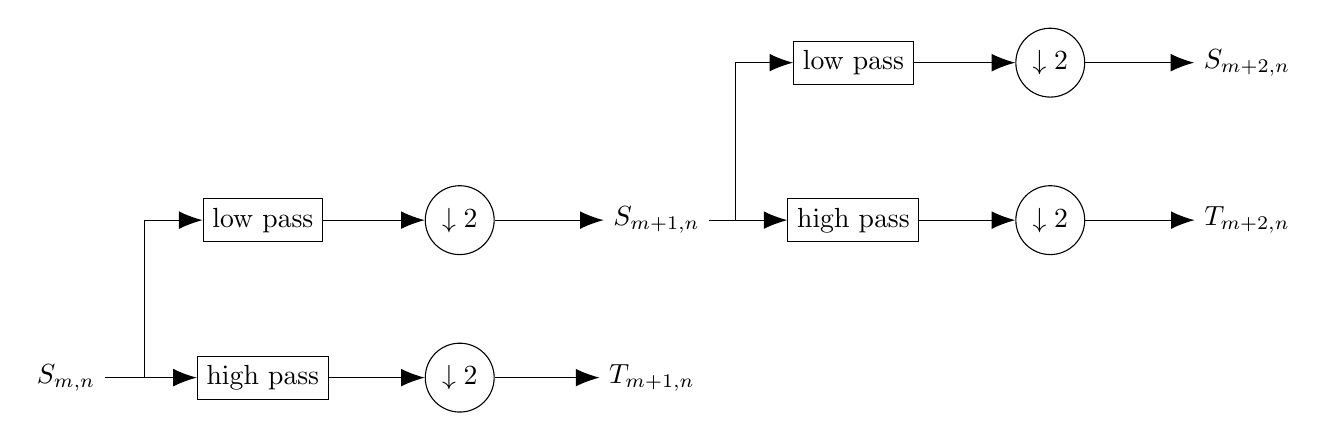
\begin{tikzpicture}

%Nodes
\node (A) at (0,0) [align=center] {$S_{m, n}$};
\node (B) at (2.5,0) [rectangle,draw] {high pass};
\node (C) at (2.5,2) [rectangle,draw] {low pass};

\draw (A) -| (1,2);
\draw[-{Latex[length=3mm]}]  (A) to (B);
\draw[-{Latex[length=3mm]}]  (1,2) to (C);

\node (D) at (5,0) [circle, draw] {$\downarrow 2$};
\node (A1) at (5,2) [circle, draw] {$\downarrow 2$};

\draw[-{Latex[length=3mm]}]  (B) to (D);
\draw[-{Latex[length=3mm]}]  (C) to (A1);

\node (E) at (7.5,0) [align=center] {$T_{m+1,n}$ };
\node (B1) at (7.5,2) [align=center]{$S_{m+1,n}$};

\draw[-{Latex[length=3mm]}]  (A1) to (B1);
\draw[-{Latex[length=3mm]}] (D) to (E);



\node (C1) at (10,4)[rectangle,draw] {low pass};
\node (C2) at (10,2)[rectangle, draw] {high pass};


\draw (B1) -| (8.5,4);
\draw[-{Latex[length=3mm]}]  (8.5,4) to (C1);
\draw[-{Latex[length=3mm]}] (B1) to (C2);


\node (D1) at (12.5,2) [circle, draw] {$\downarrow 2$};
\node (A2) at (12.5,4) [circle, draw] {$\downarrow 2$};

\draw[-{Latex[length=3mm]}] (C2) to (D1);
\draw[-{Latex[length=3mm]}] (C1) to (A2);

\node (F) at (15,4) {$S_{m+2,n}$};
\node (E1) at (15,2) [align=center] {$T_{m+2,n}$};

\draw[-{Latex[length=3mm]}] (A2) to (F);
\draw[-{Latex[length=3mm]}]  (D1) to (E1);



\end{tikzpicture}
\caption[Schematic of DWT filtering]{\textbf{Schematic of DWT filtering.} 
Diagram of the filtering of the approximation coefficients to produce the approximation and detail coefficients at successive scales.
The subsample symbold $\downarrow 2$ means take every second value of the filter signal.}
\label{fig:dwt_scheme}

\end{figure}


We can also go the opposite direction and reconstruct $S_{m,n}$ from $S_{m+1, n}$ and $T_{m+1, n}$. After some algebra one obtains 
the equation for the reconstruction algorithm

\begin{equation}
    S_{m-1, n} = \frac{1}{\sqrt{2}} \sum_k c_{n-2k} S_{m,k} + \frac{1}{\sqrt{2}} \sum_k b_{n-2k} T_{m, k}
\end{equation}

At the scale $m-1$ the approximation coefficients can be found in terms of a combination of approximation and detail coefficients at the next scale $m$. The 
reconstruction algorithm is the second half of the \textit{fast wavelet transform} (FWT). 

So far we have worked with the assumption of a continuous input signal $x(t)$ for the entire derivation of the DWT. To begin the fast wavelet transform algorithm
we need an initial set of approximation coefficients $S_{0, n}$ which are calculated using the continuous signal, see Eq. \ref{eq:approx_coef}. In practice, we don't
have access to $x(t)$ but only to a discrete sample $x[t]$. It is common practice to simply use the input signal $x[t]$ directly as approximation coefficients at 
scale $m=0$. This is formally not correct, as $S_{0,n}$ is a weighted average of $x(t)$ in the vicinity of $n$, but it works well in most cases. So as initial input 
to the filter bank simple set

\begin{equation}
    S_{0, n} = x[n]
\end{equation}
with both coefficient index and signal index have the same range $[0, T]$ and are equal to each other. There are also more elaborate preprocessing schemas to obtain 
a better set of initial approximation coefficients. A discussion of the issue can, for example, be found in \cite{strang1996wavelets}. 


Note that in literature the fast wavelet transform, discrete wavelet transform,
decomposition/reconstruction algorithm, fast orthogonal wavelet transform, multiresolution algorithm, pyramid algorithm etc. are used interchangeably. Also note that 
other discretizations of the wavelet transform are also referred to as discrete wavelet transform.

\subsection{Noise estimation and Denoising}

Now we have the introduced the mathematical machinery of the wavelet transform, we can use it to address the problems we encountered in section \ref{sec:Wiener_deconv}.
To be more precise, we needed an estimate of the noise level and an estimate of the signal without noise (or at least of the respective power spectra)
as inputs to the Wiener deconvolution filter. 
Based on papers by Donoho \cite{donoho1994ideal}, \cite{donoho1995noising} I will present a method for denoising called \textit{wavelet thresholding} or 
\textit{VISUSHRINK}.

This method assumes we have a signal with added Gaussian white noise $f + \epsilon$. It can be observed that the noisy components of the transform signal are mostly contained
in the smallest scale wavelet coefficients with low absolute values. These small coefficients are simply set to zero and then the signal is reconstructed, 
giving an estimate of the denoised signal $\tilde{f}$. Donoho shows in their work that this thresholding technique gives a good estimator of $f$ both in terms of 
minimizing the mean-squared error and $\tilde{f}$ being smooth. Because of the smooth results wavelet thresholding was greatly used in the image processing domain. 

The fact that the empirical wavelet coefficients at the finest scale are essentially pure noise is also used for the noise estimation. A robust noise estimator
is the median of the absolute deviation (MAD) of the smallest scale wavelet coefficients. In the Gaussian case this is calibrated to 
$\tilde{\sigma} = \frac{\text{MAD}}{0.6745}$. The threshold value is then set accordingly to 

\begin{equation}
    \lambda_U = (2 \ln N)^{1/2}\tilde{\sigma} = \frac{(2 \ln N)^{1/2}\text{MAD}}{0.6745}
    \label{eq:threshold_esti}
\end{equation}

This is the so-called \textit{universal threshold} and is both simple and commonly used. There are also different wavelet denoising schemas based on thresholding, such 
as \textit{soft-thresholding}, the \textit{minimax} method, various Bayesian approaches and others but hard thresholding showed good results for our use case while being
both simple and robust. 

A full description of the algorithm used to estimate the noise level and the denoised data is given in Algorithm \ref{algo:visushrink}.

\begin{algorithm}[htb]
    \hspace*{\algorithmicindent} \textbf{Input:} time series data $x_i$ of length $N$; analyzing wavelet $\psi$ \\ 
    \begin{enumerate}
        \item Apply the DWT to the input data $x_i$ to obtain the wavelet coefficients $\Theta_i^0$
        \begin{equation}
            \Theta_i^0 = \mathscr{W}_{\psi} \{x_i\}
        \end{equation}

        \item Calculate the MAD of the fine scale coefficients $\Theta_{i}^0$, the estimate of the noise level $\tilde{\sigma}$ and the universal estimator $\lambda_U$. 
        Let $\bar{\Theta} = \text{median}(\Theta_i^0)$ be the median of the fine scale coefficients and $N$ the length of the time series $x_i$
        \begin{align}
        \text{MAD} &= \text{median}(|\Theta_i^0 - \bar{\Theta}|) \\
        \tilde{\sigma} &= \frac{\text{MAD}}{0.6745} \\
        \lambda_U &= (2 \ln N)^{1/2}\tilde{\sigma}
        \end{align}

        \item Apply hard thresholding to the fine scale wavelet coefficients
        \begin{equation}
            \Theta_i^1 = \begin{cases}
                0, & |\Theta_i^0| < \lambda_U \\
                \Theta_i^0, & |\Theta_i^0| \geq \lambda_U
            \end{cases}
        \end{equation}
        \item Apply the inverse DWT to the tresholded coefficients $\Theta_i^1$ to obtain an estimate of the denoised signal $\tilde{x_i}$
        \begin{equation}
            \tilde{x_i} = \mathscr{W}_{\psi}^{-1} \{\Theta_i^1 \}
        \end{equation}
    \end{enumerate}
    \hspace*{\algorithmicindent} \textbf{Output:} estimate of the noise level $\tilde{\sigma}$; estimate of denoised signal $\tilde{x_i}$ \\ 
    \caption{The VISUSHRINK Algorithm}
    \label{algo:visushrink}
\end{algorithm}

Now we have established all the tools necessary for the inversion of the BOLD observation model. In the next chapter I will combine these and present the full algorithm
for training on fMRI data.

\chapter{Datasets, Training and Evaluation} \lhead{\emph{Datasets, Training and Evaluation}}

In this chapter I will first give a full description of the BOLD inversion teacher forcing algorithm I developed. 
Then I will showcase the datasets on which the models were trained, delve into the specifics of the training routines utilized, 
and discuss the evaluation measures I employed to assess the performance of the trained models.

\section{BOLD inversion teacher forcing}

We recall from section \ref{sec:bold_obs_eq} the BOLD observation equation

\begin{equation}
    \hat{x}_t = O(z_t, r_t) = \boldsymbol{B} \left( (hrf \ast z)_t\right) + \boldsymbol{J}r_t + \epsilon_t.
\end{equation}

To apply the teacher forcing algorithm we need to generate desired target values $d_t$ for the latent states $z_t$ from the ground truth $x_t$

\begin{equation}
    \{d_t\} = O^{-1}(\{x_t, r_t\}) = \left\{\text{Conv}^{-1}\left(\boldsymbol{B}^+ \left(x_t - \boldsymbol{J} r_t \right), hrf \right) \right\}
    \label{eq:bold_inv_naive}
\end{equation}

where $\text{Conv}^{-1}(\cdot, hrf)$ is the deconvolution of data with the $hrf$. Note that we to perform these steps on an entire series $\{x_t\}$
because there is no one-to-one correspondence between a time point $t$ of the unconvoluted and convoluted time series.

The issue with solving the inversion with equation \ref{eq:bold_inv_naive} is that the deconvolution has to be performed in every epoch of training because $B$ is 
learned and doesn't stay constant. The trick is to notice that the same $hrf$ function is applied to all latent space dimensions, hence one can interchange the matrix 
multiplication with $\boldsymbol{B}$ and the convolution step.

Let $Z_{i,t} \in \mathbb{R}^{M \times T}$ be the data matrix of the $M$-dimensional time series of length $T$, $hrf[t] = h_t$ be the hrf vector at an arbitrary
but fixed repeat time and $\boldsymbol{B} = b_{ij} \in \mathbb{R}^{N \times M}$ the observation matrix.

\begin{align}
    \boldsymbol{B} ( hrf \ast Z)_t &= \sum_{i=1}^{M} b_{ij} \sum_{\tau=1}^{T} h_{t - \tau} Z_{j, \tau}  \\
                      &= \sum_{i=1}^{M} \sum_{\tau=1}^{T} h_{t - \tau} b_{ij} Z_{j, \tau} \\
                      &= \sum_{\tau=1}^{T} h_{t - \tau} \sum_{i=1}^{M}  b_{ij} Z_{j, \tau} \\
                      &= \left(hrf \ast (\boldsymbol{B} \cdot Z) \right)_t
\end{align}

Furthermore, we can pull the nuisance variables $r_t$ through the convolution using linearity (see Proposition \ref{prop:conv_properties}). Let $r_t$ be the nuisance variables
and $r_{\text{deconv}_t} = \text{Conv}^{-1}(r_t, hrf)$ the deconvoluted nuisance variables.

\begin{align}
    O(z_t, r_t) &= \boldsymbol{B} \left( (hrf \ast z)_t\right) + \boldsymbol{J}r_t \\
                &= \left(hrf \ast (\boldsymbol{B} \cdot z) \right)_t + \boldsymbol{J}r_t \\
                &= \left(hrf \ast (\boldsymbol{B} \cdot z + \boldsymbol{J} \cdot \text{Conv}^{-1}(r_t, hrf) \right)_t \label{eq:obs_eq_simple}
\end{align}

Equation \ref{eq:obs_eq_simple} now has an inversion, which is computationally much more efficient:

\begin{equation}
    \{d_t\} = O^{-1}(\{x_t, r_t\}) = \{\boldsymbol{B}^{+} \left( \text{Conv}^{-1}(x_t, hrf) - \boldsymbol{J} \cdot \text{Conv}^{-1}(r_t, hrf) \right) \}
\end{equation}

This form lets us compute the deconvoluted time series $\text{Conv}^{-1}(x_t, hrf)$ and \newline $\text{Conv}^{-1}(x_t, hrf)$ once before training. At train time only the 
psuedo-inverse $\boldsymbol{B}^+$ has to be computed and applied as in inversion TF (see Eq. \ref{eq:inversion_tf}).

To compute the deconvolution, first the VISUSHRINK algorithm (see Algorithm \ref{algo:visushrink}) is applied to the time series $\{x_t\}$ to obtain an estimate of the 
noise level $\tilde{\sigma}$ and the denoised signal $\tilde{x_i}$. Then the power spectra of the measured signal, the denoised signal, the noise and the $hrf$
are calculated and used in the Wiener deconvolution filter (see Eq. \ref{eq:wiener_deconv}).
Note that the noise is assumed to be Gaussian white noise, hence the power spectrum is flat $P_i = \tilde{\sigma}^2$.

The Wiener filter is then applied to the observed signal in Fourier space and the result transformed back to the time domain, resulting in the deconvoluted 
time series $\{x_t\}_{deconv}$.

\subsection{Boundary issues and minimum noise level}

There are issues at the boundaries of a signal batch when calculating the deconvolution there. A batch refers to a subset of the dataset. 
Instead of feeding the entire dataset into the model at once in training, the time series data is divided into several batches, 
and the model is trained on each batch one at a time.

The reason is that values from outside the batch were used to calculate 
the values at the edges. The convolution effectively lets information smear out across time. We do however not have access to values from outside the batch and thus
there are typically large errors at the edges of the deconvoluted signal.

Ideally we would cut off the boundaries and only use valid points, i.e. ignore the first and last $\text{length}(hrf)$ points of each batch. In the context of fMRI we are 
however already heavily data constrained with time series of length $\mathcal{O}(10^3)$. In relation to this the length of the $hrf$ impulse is not negligible. For 
example, we have $\text{length}(hrf_{2.0}) = 17$, $\text{length}(hrf_{1.4}) = 27$ and $\text{length}(hrf_{0.8}) = 41$. We can't afford to drop that many data points 
\textit{in each batch}. 

From visual inspection of the deconvolution results, I decided to cut $\frac{1}{4} \text{length}(hrf)$ at the boundaries, as the 
biggest error occur there. The hyperparameters \textbf{cut\_l} and \textbf{cut\_r} set how much of the left and right boundary is cut. The cutoffs of a batch 
are visualized in the figures \ref{fig:high_freq_issues} and \ref{fig:min_conv_noise}.  

In practice, the noise estimation only has a finite precision. For very small noise levels, for example in strongly preprocessed data or even no noise in artificial 
benchmark data, the deconvolution described above encounters numerical issues. The Wiener filter begins to return high frequency artifacts if we let the noise level 
approach $0$ (see figure \ref{fig:high_freq_issues}).  In most experimental cases this should not occur, but noiseless benchmark data and heavily smoothed data 
cause the noise estimation to return values close to $0$.
A hyperparameter \textbf{min\_conv\_noise} is set which is the minimum $\tilde{\sigma}$ the Wiener filter uses to avoid high frequency artifacts. Figures 
\ref{fig:high_freq_issues} and \ref{fig:min_conv_noise} offer a comparison between the simple Wiener filter and one with added minimum noise level. The 
higher frequency oscillations disappear, only the boundaries still contain large deviations from the original signal.

\begin{figure}
    \centering

    \begin{subfigure}[b]{\textwidth}
        \centering
        \includegraphics[width=\textwidth]{Images/high_freq_issues.png}
        \caption{Deconvolution of a Lorenz63 time series with no noise component. Deconvolution returns high frequency artifacts both at the 
                 boundaries and throughout the signal.}
        \label{fig:high_freq_issues}
    \end{subfigure}

    \begin{subfigure}[b]{\textwidth}
        \centering
        \includegraphics[width=\textwidth]{Images/min_conv_noise.png}
        \caption{Deconvolution of a Lorenz63 time series with no noise component, but minimum noise level set. High frequency artifacts are much smaller and only 
                appear close to the boundaries within the $\frac{1}{4}\text{length}(hrf)$ cutoffs.}
        \label{fig:min_conv_noise}
    \end{subfigure}

       \caption[Deconvolution issues exemplified by a Lorenz63 time series]{Deconvolution issues exemplified by a Lorenz time series}
       \label{fig:three graphs}
\end{figure}

A full description of the deconvolution algorithm which was finally implemented and used for the experiments is given in Algorithm \ref{algo:deconv_full}.

\begin{algorithm}[htb]

    \hspace*{\algorithmicindent} \textbf{Input:} time series data $x_i$ of length $N$; analyzing wavelet $\psi$;\\ \hspace*{\algorithmicindent} \phantom{Input:  } minimum noise level $\tilde{\sigma}_{min}$;
    boundary cutoffs cut\_l, cut\_r;  \\ 
    \begin{enumerate}
        \item Apply the VISUSHRINK algorithm (see Algorithm \ref{algo:visushrink}) to the time series $\{x_t\}$ to obtain an estimate of the 
        noise level $\tilde{\sigma}$ and the denoised signal $\tilde{x_i}$

        \item \textbf{If} $\tilde{\sigma} < \tilde{\sigma}_{min}$ \textbf{then} Set $\tilde{\sigma} := \tilde{\sigma}_{min}$

        \item Compute the Fourier transform of the $hrf$ and the power spectra of the observed signal, the denoised signal 
              and the noise. The noise is assumed to be Gaussian white noise, hence the power spectrum is flat $P_i = \tilde{\sigma}^2$.

        \item Compute the Wiener filter (see Eq. \ref{eq:wiener_deconv}). The power spectrum of the denoised signal is used as input
              $S(k)$, the power spectrum of the original signal in Eq. \ref{eq:wiener_deconv}.
        
        \item Apply the Wiener deconvolution filter (see Eq. \ref{eq:wiener_filter_fourier}) to measured signal in Fourier space
        
        \item Transform the result back to the time domain to obtain $\{x_t\}_{deconv}$.
        
        \item Edges of signal are set to NaN as they contain artifacts and can't be used. \newline
              $x \left[\text{begin}:\text{begin} + \text{cut\_l} \right] = \text{NaN}$, $x \left[\text{end}-\text{cut\_r}:\text{end}\right] = \text{NaN}$
    \end{enumerate}
    \hspace*{\algorithmicindent} \textbf{Output:} estimate of the deconvoluted signal $\{x_t\}_{deconv}$;\\ 
    \caption{The full deconvolution Algorithm}
    \label{algo:deconv_full}
\end{algorithm}

\section{Evaluation metrics} \label{sec:eval_metrics}

There is a major problem when evaluating the performance of models on chaotic time series. It can easily be seen when remembering the concept of Lyapunov exponents 
(c.f. \ref{sec:lya_exp}). If the maximum Lyapunov exponent of a system is larger than $0$, $\lambda_{\max} > 0$, which is a necessary condition of chaos, nearby trajectories
diverge exponentially quickly. This limits the applicability of $n$-step ahead prediction errors, as even small numerical errors will lead to exponentially growing 
prediction errors.

We therefore need different tools to evaluate the performance of models trained on chaotic time series which depend on properties invariant to the initial conditions.
In this work, I will use two measures that have been established (\cite{mikhaeil2022difficulty}) to robustly evaluate the performance on chaotic data. 
The first is a state space measure that focuses on geometric properties of the time series and the other is based on the power spectrum. 

\subsection{State Space Distance \texorpdfstring{$D_{stsp}$}{Lg}} \label{sec:d_stsp}

The general idea of this measure was introduced in \cite{koppe2019identifying}. 
Given an observed $N$-dimensional time series $\{x_t\}$ of length $T$ and a
time series $\{\hat{x}_t\}$ with the same dimension/length generated by a model aiming to reconstruct the dynamical system underlying $\{x_t\}$, $D_{stsp}$ measures
the geometrical overlap of orbits in state space.

For low dimensional systems $N \leq 6$ the state space is separated into $k^N$ bins where $k$ is the number of bins per dimension. Each bin is given a label $i$ and 
the number of points $n_i$ of the time series is within that bin is measured. This gives us the relative frequency of that bin

\begin{equation}
    p_i = \frac{n_i}{T}.
    \label{eq:rel_freq}
\end{equation}

Combining these frequencies across all bins in space results in a probability distribution which approximates the state space distribution of the underlying dynamical system.
Then the Kullback-Leibler-Divergence (KLD) of the empirical distributions can be calculated to give a measure of the overlap of both systems in state space:

\begin{equation}
    D_{stsp} = \sum_{i=1}^{k^N} p_i \log \left(\frac{p_i}{q_i}\right)
\end{equation}

where $p_i$ are the relative frequencies of the measured time series and $q_i$ are the relative frequencies of the generated time series. Note that KLD is not a metric in 
the mathematical sense, but instead it is a divergence which establishes the separation of probability distributions.

The complexity of this binning approach scales exponentially with the observation dimension $N$ and thus becomes intractable with growing $N$. To compute $D_{stsp}$ in higher 
dimensional systems, \cite{brenner2022tractable} use a Gaussian mixture model with centers (means) $x_t$ and diagonal covariance 
$\boldsymbol{\Sigma}=\text{diag}(\sigma^2, \cdots, \sigma^2)$ where $\sigma$ is a hyperparameter. The GMMs of a time series are given by 

\begin{equation}
    f(y) = \frac{1}{T} \sum_{t=1}^{T} \mathcal{N}(y;x_t,\boldsymbol{\Sigma}).
\end{equation}

Following \cite{hershey2007approximating}, the KLD of the two GMMS can be computed using a Monte-Carlo sampling approach 

\begin{equation}
    D_{stsp} \approx \frac{1}{K} \sum_{i=1}^{K} \log \left(\frac{f_{obs}(y_{i})}{f_{gen}(y_{i})}\right) 
             = \frac{1}{K} \sum_{i=1}^{K} \log \Bigg ( \frac{1/T \sum_{t=1}^{T} \mathcal{N}\left( y_i;x_t;\boldsymbol{\Sigma}\right)}{1/T \sum_{t=1}^{T} \mathcal{N}\left(y_i;\hat{x}_t;\boldsymbol{\Sigma}\right)}\Bigg )
\end{equation}

where $K$ is the number of samples drawn, $f_{obs}$ is the distribution of the observed time series and $f_{gen}$ is the distribution of the generated time series.
This approach can be interpreted as an adaptive binning approach only considering bins with points in them. While the two measures correlate strongly in low dimensions,
it is difficult to validate the GMM approach in high dimensional systems.

\subsection{Power Spectrum Error \texorpdfstring{$D_{PSE}$}{Lg}} \label{sec:d_pse}

The previously introduced state space measures discards all temporal structure of the data. To include temporal information in the model evaluation I will also use the 
power spectra of the observed and generated time series. For each dimension $i \in [\![0, N]\!]$ the scalar time series $\{x^{(i)}_t\}$ can be used to 
calculate a power spectrum density (PSD) $\{S^{(i)}_k\}$. The components are calculated from the Fourier transform of $\{x^{(i)}_t\}$.

\begin{equation}
    S_k^{(i)} = \frac{|\widehat{x}^{(i)}_k|}{T} = \frac{| \mathscr{F}\{x^{(i)}_t\}_k |}{T}
\end{equation}

To evaluate the agreement of power spectra the Hellinger Distance (HD) is used as suggested by \cite{mikhaeil2022difficulty}. Since HD is a probability measure 
the computed power spectra have to be normalized:

\begin{equation}
    \bar{S}^{(i)}_k = \frac{S^{(i)}_k}{\sum_{j=1}^{T}S^{(i)}_j}
\end{equation}

The Hellinger Distance is then calculated as follows using the power spectra of the observed time series  $p^{(i)}_k = \bar{S}^{(i)}_k(\{x^{(i)}_t\})$ and 
the generated time series $q^{(i)}_k = \bar{S}^{(i)}_k (\{\hat{x}^{(i)}_t\})$

\begin{equation}
    D_H^{(i)} = \sqrt{1 - \sum_{k = 1}^{T}\sqrt{p^{(i)}_i q^{(i)}_i}}
    \label{eq:hellinger_dist}
\end{equation}

The power spectrum error is computed by averaging the Hellinger Distances across all $N$ dimensions of the observed system.

\begin{equation}
    D_{PSE} = \frac{1}{N} \sum_{i = 1}^{N} D_H^{(i)}
    \label{eq:d_pse}
\end{equation}

Before any computations the power spectra typically have to be smoothed with a Gaussian kernel with width $\sigma$ to reduce the noise. This is another 
hyperparameter that has to be chosen to evaluate a model.

\section{Datasets}

The methods developed in this thesis are applied to both synthetic benchmark datasets and real world datasets. As benchmark system I used the Lorenz63 system which 
was convoluted different $hrf$ functions and obfuscated with different noise levels. The advantage of such a benchmark system is that the latent, 
(unconvoluted and noiseless) trajectories of the system are known. This allows us to evaluate the model outputs both in the latent space and the observation or 
measurement space. As real fMRI data I used the publicly available dataset by the MPI Leipzig (\cite{babayan2019mind}), which contains task-free 
resting-state fMRI (rs-fMRI) of 227 healthy participants together with range of physiological measurements, cognitive tests and emotion/personality tests.

\subsection{Lorenz63 System}

The Lorenz63 introduced in \cite{lorenz1963deterministic} was designed to describe atmospheric convection based on three observables. A two-dimensional fluid layer is 
uniformly warmed from below and cooled from above. It is a continuous dynamical system given by the following set of differential equations:

\begin{align}
    \frac{dx_1}{dt} &= \sigma (x_2 - x_1) \\
    \frac{dx_2}{dt} &= x_1 (\rho - x_3) - x_2 \\
    \frac{dx_3}{dt} &= x_1 x_2 - \beta x_3  
\end{align}

where $x_1$ is proportional to the rate of convection, $x_2$ to the horizontal temperature variation and $x_3$ to the vertical temperature variation. The constants 
are $\alpha$, $\rho$ and $\beta$ are system parameters proportional to the Prandt number, Rayleigh number and certain physical dimensions of the fluid-layer. To produce 
chaoticity the following parameters are typically used: $\sigma=10$, $\rho=28$ and $\beta = \frac{8}{3}$. These settings produce the so-called "butterfly attractor" 
characteristic of the Lorenz system. Example trajectories are shown in Figure \ref{fig:lorenz_system}.

\begin{figure}
    \includegraphics[width=\textwidth]{Images/lorenz_system.png}
    \caption[Simulated data of the Lorenz System]{\textbf{Simulated data of the Lorenz System: } Example trajectories with 1000 time steps. 
    Lorenz attractor with characteristic butterfly wing shape in 3D state space}
    \label{fig:lorenz_system}
\end{figure}

\subsection{LEMON Dataset}

The LEMON ("Leipzig Study for Mind-Body-Emotion Interactions") dataset is a publicly available dataset published by the MPI Leipzig \cite{babayan2019mind}. 
It consists of 227 healthy participants divided into a young ($N=153$) and an elderly group ($N=74$). Each of the participants completed a battery of tests for
physiological assessment, including 6 cognitive tests and 18 emotion- and personality-related questionnaires, a 62-channel EEG experiment at rest and 
a task-free resting-state fMRI scan while further physiological measures were continuously acquired (blood-pressure, heart-rate, pulse, respiration). The full details of 
the dataset and the data acquisition can be found in \cite{babayan2019mind}.

In this work I will solely focus on the rs-fMRI data and not use the other data modalities for training the models. Utilizing the preprocessed fMRI data in the dataset,
time series from 16 regions of interest (ROIs) were extracted. These time series were subsequently smoothed, band-pass filtered and standardized to have a mean of 0 and
a standard deviation of 1. This routine was copied from \cite{koppe2019identifying} which provides more details on the preprocessing.
Example trajectories are shown in figure \ref{fig:fmri_example}.

\begin{figure}
    \includegraphics[width=\textwidth]{Images/fmri_example_traj.png}
    \caption[Example trajectories of fMRI time series]{First 8 dimensions of a resting state fMRI time series from the LEMON dataset}
    \label{fig:fmri_example}

\end{figure}

\FloatBarrier
\section{Experimental Setup: Benchmarking on Lorenz63 data}

To benchmark the BOLD inversion algorithm and provide a proof of concept I used the following two setups:

\subsection{Benchmarking on data without noise}\label{sec:noiseless_lorenz}
\begin{enumerate}
    \item I simulated the Lorenz63 system in the chaotic regime to create a dataset containing $10^5$ time steps.
    
    \item I trained a shallowPLRNN model with 5000 epochs on this dataset using weak identity teacher forcing and the identity mapping as observation model.

    \item Using the model training in the previous step I created 4 datasets, each containing 100 trajectories of length $1.1 \cdot 10^6$ drawn from the model. The initial conditions
          were slightly perturbed with Gaussian white noise ($\mu=0, \sigma=1$) and the first $10^5$ time steps discarded to ensure the model has reached its limiting set.

          In the linear case I did not further modify the data. In the other cases I convoluted the data with an $hrf_{1.2}$, an $hrf_{0.5}$ and an $hrf_{0.2}$ respectively.
          These datasets were split 50:50\% as training and test set for the benchmark.

    \item To benchmark, I trained 100 models with the linear identity mapping on each of the datasets. Next, I trained 100 models with BOLD observation model on each dataset.
          For the impulse response I used the same $hrf$ used to generate the dataset. In the case of the linear data without any convolution I used the $hrf_{1.2}$. 
          Each model was trained for 1000 epochs.

    \item After every 25 training epochs a trajectory is generated by the model and the state space distance $D_{stsp}$ and the power spectrum error $D_{PSE}$ are calculated
          so that we have access to the evolution of the Loss, $D_{stsp}$ and $D_{PSE}$ across training when evaluating the benchmark.
\end{enumerate}

A visualization of these convoluted datasets is shown in figure \ref{fig:lorenz_conv}. The complete hyperparameter settings of the training, 
such as the used optimizer, batch size etc. is given in the appendix, table \ref{tab:args lorenz runs}.

\begin{figure}
    \includegraphics[width=\textwidth]{Images/lorenz_conv.png}
    \caption[Convolution of the reconstructed Lorenz attractor with different $hrf$-functions]
    {Convolution of the reconstructed Lorenz attractor with different $hrf$-functions}
    \label{fig:lorenz_conv}

\end{figure}

\subsection{Benchmarking on data with noise}\label{sec:noisy_lorenz}
\begin{enumerate}
    \item I simulated the Lorenz63 system in the chaotic regime to create a dataset containing $10^5$ time steps

    \item I trained a shallowPLRNN model with 5000 epochs on this dataset using weak identity teacher forcing and the identity mapping as observation model.
    
    \item Using the model trained in the previous step I created 8 datasets, each containing 100 trajectories of length $1.1 \cdot 10^5$ drawn from the model. The initial conditions
          were slightly perturbed with Gaussian white noise ($\mu=0, \sigma=1$) and the first $10^4$ time steps discarded to ensure the model has reached its limiting set.

          In the linear case I added Gaussian white noise to two datasets, once with $\sigma=0.01$ and once with $\sigma=0.1$. For the others I convoluted two datasets 
          each with an $hrf_{1.2}$, an $hrf_{0.5}$ and an $hrf_{0.2}$ respectively. Then I again added Gaussian white noise to the datasets, 
          once with $\sigma=0.01$ and once with $\sigma=0.1$. These datasets were split 50:50\% as training and validation set for the benchmark.

    \item To benchmark, I trained 100 models with the BOLD observation model on each dataset with the respective impulse response used to create the dataset. I also trained 
          with all three impulse responses, $hrf_{1.2}$,  $hrf_{0.5}$ and $hrf_{0.2}$ on the unconvoluted datasets.

    \item After every 25 training epochs a trajectory is generated by the model and the state space distance $D_{stsp}$ and the power spectrum error $D_{PSE}$ are calculated
          so that we have access to the evolution of the Loss, $D_{stsp}$ and $D_{PSE}$ across training when evaluating the benchmark. The generated trajectories have the same
          length as the trajectory from the test set, $5\cdot 10^4$ in this case.
\end{enumerate}

\begin{figure}
    \includegraphics[width=\textwidth]{Images/lorenz_conv_noise.png}
    \caption[Example of noisy convoluted Lorenz attractor]{Example of noisy convoluted Lorenz attractor}
    \label{fig:lorenz_conv_noise}
\end{figure}

An example of these noisy trajectories is shown in figure \ref{fig:lorenz_conv_noise}. Again, the list of hyperparameters are given in table \ref{tab:args lorenz runs}.

\section{Experimental Setup: Filtering LEMON datasets} \label{sec:filter_lemon}

When investigation the time series of the LEMON datasets I noticed the training results varied greatly between participants. Evaluating models trained with the same hyperparameters
on different participants returned different very large differences on the validation set, which was chosen as the last 25\% of the data points.

\begin{figure}
    \includegraphics[width=\textwidth]{Images/high_var_patient_pe_comparison.png}
    \caption[Prediction Error on test set differing strongly between participants]
    {\textbf{Prediction Error on test set differing strongly between participants: } Distribution of prediction errors on two different participants ($N=398$). The prediction capability of
    the models trained on participant 003 (\textit{blue}) is significantly worse than those trained on participant 004 (\textit{orange}). Set of hyperparameters for training did not 
    differ between participants.}
    \label{fig:high_var_patient_pe_comparison}
\end{figure}

Following a suggestion by Alena Brändle I looked at the moving averages and moving variances of the time series to see how they evolve with time. Given a window size $w$,
an $N$ dimensional time series $\{x_t\}$ and a dimension $i \in [\![0, N]\!]$  the simple moving average ($SMA$) and variance ($SMV$) are calculated as follows

\begin{align}
    SMA_k^{(i)} &= \frac{1}{w} \sum_{t=k}^{k+w} x_t^{(i)} \\
    SMV_k^{(i)} &= \frac{1}{w} \sum_{t=k}^{k+w} (x_t^{(i)} - SMA_k)^2
\end{align}

Then we average over all dimensions:

\begin{align}
    SMA_k = \frac{1}{N} \sum_{i=1}^{N} SMA_k^{(i)} \\
    SMV_k = \frac{1}{N} \sum_{i=1}^{N} SMV_k^{(i)}
\end{align}

This results in two scalar time series that can easily be visualized and give us an intuition how the underlying fMRI time series evolves. This does however introduce a 
hyperparameter, the window size $w$. There is no simple criterion to decide on a window size. A large window will oversmooth the data while a small window will result 
many noise artifacts remaining. I chose a window size $w=40$ are is delivered good results upon visual inspection.
In figure \ref{fig:sma_smv_example} the SMA and SMV for different participants are shown. Clearly, the variance is not constant but varies greatly 
throughout time. Constant variance, however, is a necessary condition for stationarity. 

\begin{figure}
    \includegraphics[width=\textwidth]{Images/example_sma_smv.png}
    \caption[Simple moving average and variance of different participants]{\textbf{Simple moving average and variance of different participants: } Example of SMA and SMV plotted
    for the first 4 participants in the LEMON dataset (participant 1 is not in the data). Window size $w=40$, the mean of the SMV is subtracted to center it around 
    $0$ and improve presentation.}
    \label{fig:sma_smv_example}
\end{figure}

To quantify the relationship between variance and time I calculated the correlation between them for each participant's SMV. The result is shown in the figure \ref{fig:smv_cor_histo}.

\begin{figure}
    \includegraphics[width=\textwidth]{Images/smv_cor_histo.png}
    \caption[Correlation between time and moving variance]{\textbf{Correlation between time and moving variance: } Normalized histogram of the Pearson correlation between time 
    and moving variance of the time series in the LEMON dataset. Window size $w=40$, bin size $b=0.04$.}
    \label{fig:smv_cor_histo}
\end{figure}

I chose to filter the LEMON dataset by only including the participants with a correlation of less than $0.16$ (the 8 center bins around 0 in the histogram). This leaves 
51 participants for the further experiments in this thesis. The time series are always split 75:25\% into training and test set and the test set is always the 
last 25\% of time points.

\section{Evaluation Setup: Choosing hyperparameters for \texorpdfstring{$D_{stsp}$}{ Lg} and \texorpdfstring{$D_{PSE}$}{Lg}} \label{sec:eval_metrics_param}

As mentioned in the introduction of the metrics $D_{stsp}$ and $D_{PSE}$ in sections \ref{sec:d_stsp} and \ref{sec:d_pse}, they each require a hyperparameter. 
In the case of $D_{stsp}$ this is the scaling parameter of the GMM, in the case of $D_{PSE}$ this is the smoothing $\sigma$ Gaussian kernel used to smooth the 
power spectra. In \cite{brenner2022tractable} these parameters are set to 1.0 and 20 respectively. Unlike the datasets used in \cite{brenner2022tractable}, 
the fMRI time series have the disadvantage of being rather short, $\mathcal{O}(10^3)$ time steps, which has implications for the choice of metric hyperparameters.

To illustrate this, I employed a model trained on the LEMON dataset to generate trajectories for two distinct time lengths: $T=100$ and $T=10^5$. In each case,
I perturbed the initial conditions and applied a noise level of $\sigma=0.07$ to these trajectories. Additionally,
I generated purely random white noise with a standard deviation of $\sigma=0.7$,
approximately matching the standard deviation of the model-generated trajectories.

Subsequently, I computed the metric $D_{stsp}$ for these diverse time series, using various scaling parameters. Specifically, 
I chose scaling factor values $scal$ within the interval $[0.1, 2]$, using a step size of $\delta = 0.01$. 
For each value of $scal$, I generated 100 distinct sets of perturbed sample trajectories and white noise samples. 
I then recorded both the mean and standard deviation of $D_{stsp}$ for each set. The comprehensive results are shown in Figure \ref{fig:dstsp_comp}.

\begin{figure}
    \includegraphics[width=\textwidth]{Images/dstsp_comp.png}
    \caption[$D_{stsp}$ dependence on scaling parameter]{\textbf{$D_{stsp}$ dependence on scaling parameter: } $D_{stsp}$ values in dependence of the scaling 
    parameter. Generating model was trained on a 16-dimensional rs-fMRI time series from the LEMON dataset.}
    \label{fig:dstsp_comp}
\end{figure}

It is clear that $D_{stsp}$ values vary much stronger in the short time series and for lower $scal$ values. For higher $scal$-values it however becomes harder to differentiate 
between purely random noise and meaningful trajectories. For lower $scal$-values the variance of $D_{stsp}$ is rises, but the white noise data is differentiated more clearly. 
In this evaluation I chose a value of $scal=0.3$.

To pick a good $\sigma$ which is used in the Gaussian kernel to smooth the power spectra I plotted the normalized smoothed power spectra of a long time series and a short
time series in figure \ref{fig:power_spectrum_sigma_comp}. It is clear that $\sigma=20$, while a good choice in the case of long time series,
is too large for short time series as it results in an over-smoothed spectrum. For the evaluation I chose the value $\sigma=2$, as this value still preserves 
the main peaks on the left plot while still reducing the small fluctuations very effectively.

\begin{figure}
    \includegraphics[width=\textwidth]{Images/power_spectrum_sigma_comp.png}
    \caption[Normalized and smoothed power spectra for different $\sigma$]{\textbf{Normalized and smoothed power spectra for different $\sigma$: }  Power spectra of the first
    observation dimension for different smoothing $\sigma$ values. Generating model was trained on a 16-dimensional rs-fMRI time series from the LEMON dataset.}
    \label{fig:power_spectrum_sigma_comp}
\end{figure}


\section{Grid search on LEMON dataset}

To find good hyperparameters for training on fMRI datasets as opposed to the benchmark datasets, I decided to run a grid search for the weak teacher forcing $\alpha$ 
and the latent dimension $\ell$. These two parameters are of special interest to us. The $\alpha$-value determines the influence of the here developed BOLD inversion algorithm,
which we want to test in this work. 
The latent dimension $\ell$ is of interest because we would like to know how many latent variables are needed to successfully reproduce the dynamics 
observed in the fMRI trajectories and how many of the observed regions of interest (ROIs) contain redundant information.

The latent dimension $\ell$ was varied from 8 to 24 in steps of 4 (remember that we are working with 16 observables), the values for $\alpha$ were chosen from 
\newline $\{0, 0.01, 0.03, 0.05, 0.1, 0.15, 0.2, 0.25, 0.3\}$ to compare no teacher forcing with $\alpha$-values 
over two orders of magnitude ($\mathcal{O}(10^{-2})$ - $\mathcal{O}(10^{-1})$).

The grid search was run on the first 10 participants from the filtered LEMON dataset with 10 models being trained per participant and parameter configuration and 
train-test split of 75:25. The detailed hyperparameter settings are given in the appendix in table \ref{tab:args lemon runs}.

Using results from this grid search, see section \ref{sec:results_gridsearch} for the evaluation, I trained on the entire (filtered) LEMON dataset. On each of the 51
participants 20 models were trained. The results are discussed in section \ref{sec:results_main_run}.



\FloatBarrier
\chapter{Results} \lhead{\emph{Results}}

\section{Results on the benchmark systems}

\subsection{Noiseless data}

These are the results for the trajectories generated from the noiseless Lorenz systems described in section \ref{sec:noiseless_lorenz}.
For the analysis, I chose the models trained for 1000 epochs. I treated a model run as not converged if the 
$D_{stsp}$ is larger than 1. Those runs were not included in the quantitative analysis summarized in table \ref{tab:noiseless_comp_table}. The distributions 
of the state space divergence and the power spectrum error are additionally displayed in figures \ref{fig:Comparison_D_stsp_noiseless} and \ref{fig:Comparison_D_PSE_noiseless}. 
The non-convergent runs are grouped together at $-0.2$ on the histograms, thereby constraining the range of bins to enhance visualization.

The results overall are as intended. On the unconvoluted dataset, the linear observation model performs better while on the convolutional datasets the convolutional
observation model outperforms. The performance disparity grows with decreased repeat time as a lower repeat time degrades the Lorenz attractor more heavily. It is noticeable 
for both models that the number of failed model runs increases with a stronger degradation of the observed trajectories. At $hrf_{0.2}$ the linear model doesn't converge
reliably at all anymore (defined as $D_{stsp}<1$). Reviewing the training in this case shows a lack of stability. There are individual epochs with good fits, but the model 
never converges there, but jumps back to a worse fit a few training epochs later. This is showcased qualitatively in figure \ref{fig:traj_gen_3d}.

\begin{figure}
    \includegraphics[width=\textwidth]{Images/Comparison_D_stsp_noiseless.png}
    \caption[Comparison of $D_{stsp}$ noiseless]{\textbf{Comparison of $D_{stsp}$ noiseless: } Distributions of $D_{stsp}$ of the convolutional observation model
    and the linear identity model. The bins at -0.2 are the model runs which did not converge, which is defined as models with $D_{stsp}>1$.}
    \label{fig:Comparison_D_stsp_noiseless}
\end{figure}

\begin{figure}
    \includegraphics[width=\textwidth]{Images/Comparison_D_PSE_noiseless.png}
    \caption[Comparison of $D_{PSE}$ noiseless]{\textbf{Comparison of $D_{PSE}$ noiseless: } Distributions of $D_{PSE}$ of the convolutional observation model
    and the linear identity model. The bins at -0.2 are the model runs which did not converge, which is defined as models with $D_{stsp}>1$.}
    \label{fig:Comparison_D_PSE_noiseless}
\end{figure}

\begin{table}
\caption{Quantitative comparison between linear and convolutional observation model}
\label{tab:noiseless_comp_table}
\begin{tabular}{llllll}
\toprule
Dataset & Obs model & $N_{converged}$ & 20 step PE & $D_{stsp}$ & $D_{PSE}$ \\
\midrule
Unconv & Lin & 92 & $0.0004 \pm 0.0001$ & $0.09 \pm 0.02$ & $0.06 \pm 0.01$ \\
Unconv & Conv & 94 & $0.0004 \pm 0.0001$ & $0.09 \pm 0.03$ & $0.05 \pm 0.01$ \\
$hrf_{1.2}$ & Lin & 87 & $0.0006 \pm 0.0001$ & $0.09 \pm 0.02$ & $0.05 \pm 0.02$ \\
$hrf_{1.2}$ & Conv & 88 & $0.0007 \pm 0.0001$ & $0.09 \pm 0.02$ & $0.05 \pm 0.01$ \\
$hrf_{0.5}$ & Lin & 83 & $0.0105 \pm 0.0016$ & $0.27 \pm 0.14$ & $0.08 \pm 0.03$ \\
$hrf_{0.5}$ & Conv & 90 & $0.0009 \pm 0.0001$ & $0.11 \pm 0.07$ & $0.07 \pm 0.02$ \\
$hrf_{0.2}$ & Lin & 0 & $- \pm -$ & $- \pm -$ & $- \pm -$ \\
$hrf_{0.2}$ & Conv & 63 & $0.0028 \pm 0.0004$ & $0.35 \pm 0.14$ & $0.11 \pm 0.04$ \\
\bottomrule
\end{tabular}
\end{table}


\begin{figure}
    \centering
    \begin{subfigure}[b]{0.24\textwidth}
        \centering
        \includegraphics[width=\linewidth]{Images/training_epochs/traj_gen_3d_125.png}
        \caption{At epoch 125}
        \label{fig:traj_gen_3d_125}
    \end{subfigure}%
    \begin{subfigure}[b]{0.24\textwidth}
        \centering
        \includegraphics[width=\linewidth]{Images/training_epochs/traj_gen_3d_150.png}
        \caption{At epoch 150}
        \label{fig:traj_gen_3d_150}
    \end{subfigure}%
    \begin{subfigure}[b]{0.24\textwidth}
        \includegraphics[width=\textwidth]{Images/training_epochs/traj_gen_3d_175.png}
        \caption{At epoch 175}
        \label{fig:traj_gen_3d_175}
    \end{subfigure}%
    \begin{subfigure}[b]{0.24\textwidth}
        \includegraphics[width=\textwidth]{Images/training_epochs/traj_gen_3d_200.png}
        \caption{At epoch 200}
        \label{fig:traj_gen_3d_200}
    \end{subfigure}
       \caption[Training instability in the presence of strong convolution]{\textbf{Training instability in the presence of strong convolution: } Trajectories of the training data 
       (a Lorenz attractor convoluted with an $hrf_{0.2}$) and of the model with linear observation equation at different training epochs.}
       \label{fig:traj_gen_3d}
\end{figure}
   
\subsection{Noisy data}

These are the results for the trajectories generated from the noisy Lorenz systems described in section \ref{sec:noisy_lorenz}. 
For the analysis, I chose the models trained for 1000 epochs. I treated a model run as not converged if the 
$D_{stsp}$ is larger than 1. Those runs were not included in the quantitative analysis summarized in table \ref{tab:noisy_comp_table}. The distributions 
of the metrics, state space divergence, power spectrum error and 20-step prediction error (PE), in the case of $hrf_{0.5}$ are additionally displayed
in figure \ref{fig:Comparison_hrf_0_5_noisy}. The non-convergent runs are grouped together at $-0.2$ on the histograms, 
thereby constraining the range of bins to enhance visualization.

The results are analogous to the noiseless case. The stronger the degradation of the underlying trajectories by both noise and convolution, the better the convolutional
observation model performs compared to the linear.

   
\begin{figure}
    \includegraphics[width=\textwidth]{Images/Comparison_hrf_0_5_noisy.png}
    \caption[Comparison of performance metrics on dataset convoluted with $hrf_{0.5}$ and added white noise]
    {\textbf{Comparison of performance metrics on dataset convoluted with $hrf_{0.5}$ and added white noise: } Distributions of $D_{PSE}$ and $D_{stsp}$ of the convolutional observation model
    and the linear identity model. The bins at -0.2 are the model runs which did not converge, which is defined as models with $D_{stsp}>1$.}
    \label{fig:Comparison_hrf_0_5_noisy}
\end{figure}

\begin{table}
\caption{Quantitative comparison between linear and convolutional observation model on noisy data}
\label{tab:noisy_comp_table}
\begin{tabular}{lllllll}
\toprule
Convolution & $\sigma$ & Obs model & $N_{converged}$ & 20 step PE & $D_{stsp}$ & $D_{PSE}$ \\
\midrule
$hrf_{1.2}$ & 0.01 & Lin & 78 & $0.0013 \pm 0.0001$ & $0.10 \pm 0.10$ & $0.05 \pm 0.01$ \\
$hrf_{1.2}$ & 0.01 & Conv & 80 & $0.0011 \pm 0.0001$ & $0.09 \pm 0.02$ & $0.06 \pm 0.01$ \\
$hrf_{0.5}$ & 0.01 & Lin & 84 & $0.0114 \pm 0.0014$ & $0.27 \pm 0.14$ & $0.09 \pm 0.03$ \\
$hrf_{0.5}$ & 0.01 & Conv & 90 & $0.0012 \pm 0.0001$ & $0.09 \pm 0.02$ & $0.06 \pm 0.01$ \\
$hrf_{0.2}$ & 0.01 & Lin & 1 & $0.0283 \pm 0.0000$ & $0.93 \pm 0.00$ & $0.19 \pm 0.00$ \\
$hrf_{0.2}$ & 0.01 & Conv & 90 & $0.0023 \pm 0.0001$ & $0.22 \pm 0.04$ & $0.14 \pm 0.02$ \\
$hrf_{1.2}$ & 0.1 & Lin & 86 & $0.0387 \pm 0.0002$ & $0.45 \pm 0.02$ & $0.09 \pm 0.01$ \\
$hrf_{1.2}$ & 0.1 & Conv & 85 & $0.0158 \pm 0.0001$ & $0.44 \pm 0.02$ & $0.09 \pm 0.01$ \\
$hrf_{0.5}$ & 0.1 & Lin & 92 & $0.0538 \pm 0.0015$ & $0.46 \pm 0.03$ & $0.10 \pm 0.01$ \\
$hrf_{0.5}$ & 0.1 & Conv & 84 & $0.0145 \pm 0.0001$ & $0.41 \pm 0.02$ & $0.09 \pm 0.01$ \\
$hrf_{0.2}$ & 0.1 & Lin & 2 & $0.0813 \pm 0.0007$ & $0.97 \pm 0.01$ & $0.18 \pm 0.00$ \\
$hrf_{0.2}$ & 0.1 & Conv & 84 & $0.0191 \pm 0.0002$ & $0.70 \pm 0.08$ & $0.24 \pm 0.02$ \\
\bottomrule
\end{tabular}
\end{table}


\FloatBarrier
\section{Grid search on LEMON dataset} \label{sec:results_gridsearch} 

I compiled the results of the hyperparameter search in the following tables and figures. Figure \ref{fig:grid_seach_latent_dimension} shows the mean and standard deviation
for varying the latent dimension $\ell$. The quantitative results are also displayed in table \ref{tab:gridsearch_ldim_table}. The results show that the model performs similarly 
for all the different tested $\ell$-values. The largest differences in performance are seen in the $D_{stsp}$ values. The value $\ell = 16$ has by far the lowest variation in 
$D_{stsp}$ across both train and test set. Hence, I chose $\ell=16$ as the value for training on the entire dataset.

Figure \ref{fig:grid_search_tf_alpha} shows the mean and standard deviation
for varying the teacher forcing $\alpha$. The quantitative results are also displayed in table \ref{tab:gridsearch_alpha_table}. The results are not very straightforward to
interpret. $D_{stsp}$-value improve for very low (or even 0) $\alpha$-values. $D_{PSE}$ is higher at low $\alpha$-values and is lowest $\alpha = 0.1$. The prediction errors 
are also the lowest around $\alpha=0.1$, hence I chose that $\alpha$-value for training on the entire dataset.

\begin{table}
\centering
\caption{Results of the parameter search for $\ell$ values. Model runs where excluded if the 1-step PE $>$ 1}
\label{tab:gridsearch_ldim_table}
\begin{tabular}{rrllllll}
\toprule
$\ell$ & $N_{converged}$ & Dataset & 1-step PE & 5-step PE & 10-step PE & $D_{stsp}$ & $D_{PSE}$ \\
\midrule
8 & 247 & Train & $0.16 \pm 0.14$ & $0.77 \pm 0.64$ & $0.93 \pm 0.53$ & $5.90 \pm 8.61$ & $0.35 \pm 0.11$ \\
8 & 247 & Test & $0.26 \pm 0.17$ & $1.44 \pm 0.66$ & $1.96 \pm 0.54$ & $9.85 \pm 9.67$ & $0.20 \pm 0.08$ \\
12 & 244 & Train & $0.16 \pm 0.15$ & $0.75 \pm 0.72$ & $0.87 \pm 1.14$ & $3.87 \pm 3.76$ & $0.32 \pm 0.11$ \\
12 & 244 & Test & $0.25 \pm 0.18$ & $1.46 \pm 0.60$ & $1.95 \pm 1.02$ & $7.86 \pm 5.21$ & $0.19 \pm 0.07$ \\
16 & 226 & Train & $0.20 \pm 0.20$ & $0.77 \pm 0.77$ & $0.78 \pm 0.54$ & $3.08 \pm 2.08$ & $0.30 \pm 0.10$ \\
16 & 226 & Test & $0.32 \pm 0.25$ & $1.53 \pm 0.67$ & $1.89 \pm 0.51$ & $6.86 \pm 3.13$ & $0.18 \pm 0.08$ \\
20 & 245 & Train & $0.28 \pm 0.17$ & $1.36 \pm 1.44$ & $1.40 \pm 1.48$ & $4.49 \pm 4.77$ & $0.34 \pm 0.12$ \\
20 & 245 & Test & $0.36 \pm 0.22$ & $1.88 \pm 1.44$ & $2.11 \pm 1.50$ & $8.71 \pm 7.05$ & $0.21 \pm 0.08$ \\
24 & 241 & Train & $0.25 \pm 0.15$ & $1.17 \pm 0.95$ & $1.25 \pm 0.69$ & $4.47 \pm 4.08$ & $0.34 \pm 0.13$ \\
24 & 241 & Test & $0.32 \pm 0.19$ & $1.66 \pm 1.04$ & $1.92 \pm 0.61$ & $8.95 \pm 7.45$ & $0.21 \pm 0.10$ \\
\bottomrule
\end{tabular}
\end{table}


\begin{figure}
    \includegraphics[width=\textwidth]{Images/grid_seach_latent_dimension.png}
    \caption[Grid search over latent dimension $ \ell $]
    {\textbf{Grid search over latent dimension $ \ell $: } Mean and standard deviation for the different metrics depending on the latent dimension $\ell$. Model runs 
    where excluded if the 1-step PE $>$ 1}
    \label{fig:grid_seach_latent_dimension}
\end{figure}

\begin{table}
\centering
\caption{Results of the parameter search for $\alpha$ values. Model runs where excluded if the 1-step PE $>$ 1}
\label{tab:gridsearch_alpha_table}
\begin{tabular}{rrllllll}
\toprule
$\alpha$ & $N_{converged}$ & Dataset & 1-step PE & 5-step PE & 10-step PE & $D_{stsp}$ & $D_{PSE}$ \\
\midrule
0.00 & 221 & Train & $0.29 \pm 0.15$ & $1.05 \pm 1.09$ & $1.26 \pm 1.76$ & $2.55 \pm 0.45$ & $0.39 \pm 0.09$ \\
0.00 & 221 & Test & $0.41 \pm 0.24$ & $1.31 \pm 1.02$ & $1.58 \pm 1.71$ & $4.70 \pm 1.45$ & $0.29 \pm 0.08$ \\
0.01 & 247 & Train & $0.31 \pm 0.15$ & $1.63 \pm 1.13$ & $1.42 \pm 0.70$ & $2.50 \pm 0.45$ & $0.32 \pm 0.10$ \\
0.01 & 247 & Test & $0.43 \pm 0.19$ & $2.26 \pm 1.27$ & $2.25 \pm 0.77$ & $4.98 \pm 1.64$ & $0.20 \pm 0.05$ \\
0.03 & 244 & Train & $0.26 \pm 0.17$ & $1.13 \pm 0.92$ & $1.03 \pm 0.31$ & $2.65 \pm 0.92$ & $0.27 \pm 0.09$ \\
0.03 & 244 & Test & $0.34 \pm 0.17$ & $1.81 \pm 0.81$ & $2.08 \pm 0.46$ & $6.55 \pm 2.52$ & $0.15 \pm 0.05$ \\
0.05 & 247 & Train & $0.20 \pm 0.16$ & $0.84 \pm 0.62$ & $0.87 \pm 0.31$ & $2.96 \pm 1.61$ & $0.26 \pm 0.09$ \\
0.05 & 247 & Test & $0.28 \pm 0.17$ & $1.57 \pm 0.65$ & $2.00 \pm 0.45$ & $8.09 \pm 4.16$ & $0.15 \pm 0.05$ \\
0.10 & 250 & Train & $0.09 \pm 0.06$ & $0.51 \pm 0.26$ & $0.67 \pm 0.27$ & $3.76 \pm 2.77$ & $0.25 \pm 0.08$ \\
0.10 & 250 & Test & $0.16 \pm 0.07$ & $1.25 \pm 0.33$ & $1.84 \pm 0.35$ & $9.59 \pm 4.38$ & $0.14 \pm 0.04$ \\
0.15 & 246 & Train & $0.09 \pm 0.13$ & $0.51 \pm 0.64$ & $0.67 \pm 0.55$ & $5.20 \pm 3.46$ & $0.30 \pm 0.09$ \\
0.15 & 246 & Test & $0.17 \pm 0.18$ & $1.28 \pm 0.66$ & $1.85 \pm 0.50$ & $11.23 \pm 5.32$ & $0.16 \pm 0.05$ \\
0.20 & 246 & Train & $0.09 \pm 0.12$ & $0.44 \pm 0.59$ & $0.69 \pm 0.61$ & $6.88 \pm 6.60$ & $0.34 \pm 0.11$ \\
0.20 & 246 & Test & $0.16 \pm 0.15$ & $1.24 \pm 0.54$ & $1.86 \pm 0.38$ & $12.76 \pm 7.90$ & $0.17 \pm 0.07$ \\
0.25 & 243 & Train & $0.10 \pm 0.15$ & $0.50 \pm 0.74$ & $0.88 \pm 0.95$ & $9.77 \pm 10.69$ & $0.37 \pm 0.11$ \\
0.25 & 243 & Test & $0.18 \pm 0.19$ & $1.33 \pm 0.72$ & $2.05 \pm 0.64$ & $15.32 \pm 10.97$ & $0.18 \pm 0.08$ \\
0.30 & 241 & Train & $0.10 \pm 0.15$ & $0.52 \pm 0.78$ & $0.90 \pm 0.98$ & $10.35 \pm 9.02$ & $0.41 \pm 0.12$ \\
0.30 & 241 & Test & $0.17 \pm 0.17$ & $1.33 \pm 0.63$ & $2.05 \pm 0.60$ & $16.31 \pm 10.90$ & $0.21 \pm 0.09$ \\
\bottomrule
\end{tabular}
\end{table}


\begin{figure}
    \includegraphics[width=\textwidth]{Images/grid_search_tf_alpha.png}
    \caption[Grid search over teacher forcing $\alpha$]
    {\textbf{Grid search over teacher forcing $\alpha$: } Mean and standard deviation for the different metrics depending on the teacher forcing $\alpha$. Model runs 
    where excluded if the 1-step PE $>$ 1}
    \label{fig:grid_search_tf_alpha}
\end{figure}

\FloatBarrier
\section{Analysis of the results on the LEMON dataset} \label{sec:results_main_run}

In this section I have compiled the results of training on the entire filtered (see section \ref{sec:filter_lemon}) LEMON dataset.
For that I trained 20 models on each participant with the hyperparameters $\ell = 16$ and $\alpha=0.1$, the other hyperparameters can be found in \ref{tab:args lemon runs}.

The results of the training are shown in figure \ref{fig:histograms_metrics_main_run}, which shows the distributions of the different metrics on both the training 
and the test datasets. Table \ref{tab:main_run_results} also summarizes these results in terms of mean and standard deviation of the different metrics.
\begin{table}
\centering
\caption{Quantitative Results of the PLRNN with BOLD observation model on the LEMON dataset. Model runs where excluded if the 1-step PE $>$ 1. $N_{converged}=1007$}
\label{tab:main_run_results}
\begin{tabular}{lll}
\toprule
metric & Train Data & Test Data \\
\midrule
$D_{stsp}$ & $2.84 \pm 2.49$ & $8.78 \pm 3.46$ \\
$D_{PSE}$ & $0.21 \pm 0.07$ & $0.14 \pm 0.04$ \\
1-step PE & $0.06 \pm 0.07$ & $0.17 \pm 0.33$ \\
5-step PE & $0.30 \pm 0.26$ & $1.20 \pm 0.41$ \\
10-step PE & $0.41 \pm 0.33$ & $1.78 \pm 0.38$ \\
\bottomrule
\end{tabular}
\end{table}


\begin{figure}
    \includegraphics[width=\textwidth]{Images/histograms_metrics_main_run.png}
    \caption[Distributions of metrics on train and test data]
    {\textbf{Distributions of metrics on train and test data: } Histograms of the results of each model run on the train and test data. Binning of the predictions errors 
    is identical for better visual comparison.}
    \label{fig:histograms_metrics_main_run}
\end{figure}

Looking at the histograms in figure \ref{fig:histograms_metrics_main_run} we can see that results on the test set appear worse overall, having both higher mean and 
higher variation, across all metrics, with the notable exception of $D_{PSE}$ where this relationship appears to be reversed.
I employed the Wilcoxon signed-rank test (method found in \cite{mcdonald2014handbook}, used implementation by \cite{2020SciPy-NMeth}) to establish the statistical
significance of the disparities in metric distributions between the training and test sets. The test results are gathered in table \ref{tab:wilcoxon_test_metrics_train_test}
and as expected the distributions between train and test set all differ significantly.

\begin{table}
\centering
\caption{Wilcoxon signed-rank test applied to the distribution of metrics on training and test set. Model runs where excluded if the 1-step PE $>$ 1. $N_{converged}=1007$}
\label{tab:wilcoxon_test_metrics_train_test}
\begin{tabular}{lllll}
\toprule
 & Result & p-Value & Rank sum & Z-statistic \\
Metric &  &  &  &  \\
\midrule
$D_{stsp}$ & Reject $H_0$. Distributions differ. & $<0.001$ & 2490 & -27.22 \\
$D_{PSE}$ & Reject $H_0$. Distributions differ. & $<0.001$ & 20630 & -25.25 \\
1-step PE & Reject $H_0$. Distributions differ. & $<0.001$ & 3578 & -27.10 \\
5-step PE & Reject $H_0$. Distributions differ. & $<0.001$ & 164 & -27.47 \\
10-step PE & Reject $H_0$. Distributions differ. & $<0.001$ & 99 & -27.48 \\
\bottomrule
\end{tabular}
\end{table}


To better illustrate the results I plotted an example reconstruction for all 16 dimensions in figure \ref{fig:ds_recontruction_example}. As it is not easy to get a good overview
over all 16 dimensions plotted next to each other, I used principal component analysis (PCA) to project the trajectories down to 3 dimensions, 
see figure \ref{fig:pca_traj_reconstruction}. Unfortunately the results of the PCA are also not much more insightful and don't provide much intuition on the quality of the 
reconstruction.

\begin{figure}
    \includegraphics[width=\textwidth]{Images/ds_recontruction_example.png}
    \caption[Exemplary DS reconstruction in a sample subject]
    {\textbf{Exemplary DS reconstruction in a sample subject: } Trajectory generated by a model (\textit{green}) compared to a real trajectory. The model was trained on the
    \textit{blue} data. The test data (\textit{orange}) was not seen by the model in training.}
    \label{fig:ds_recontruction_example}
\end{figure}

\begin{figure}
    \includegraphics[width=\textwidth]{Images/pca_traj_reconstruction.png}
    \caption[Trajectories projected down to the first 3 principal components]
    {\textbf{Trajectories projected down to the first 3 principal components: } Trajectory generated by a model (\textit{orange}) compared to a real trajectory (\textit{blue}).
    The first 3 principal components of the true data are used.}
    \label{fig:pca_traj_reconstruction}
\end{figure}

When looking at different model runs it can be observed that a low $D_{stsp}$ value and a low $D_{PSE}$ often don't coincide.
In figure \ref{fig:metric_trajectory_comparison} I plotted some examples of trajectories with different combinations of high/low $D_{stsp}$ and $D_{pse}$ values to examine 
what these differences mean for the reconstruction.

\begin{figure}
    \includegraphics[width=\textwidth]{Images/metric_trajectory_comparison.png}
    \caption[Comparison of trajectories with different $D_{stsp}$ and $D_{PSE}$ combinations]
    {\textbf{Comparison of trajectories with different $D_{stsp}$ and $D_{PSE}$ combinations: } Trajectories and power spectra generated by models (\textit{orange}) with different 
    $D_{stsp}$ and $D_{PSE}$ values compared to the real trajectories (\textit{blue}).}
    \label{fig:metric_trajectory_comparison}
\end{figure}

From looking at the different examples shown in figure \ref{fig:metric_trajectory_comparison} it is immediately apparent that a high $D_{stsp}$ and $D_{PSE}$ result in 
a bad model which isn't able to reconstruct the dynamics at all. In the case of a low $D_{stsp}$ combined with a high $D_{PSE}$ the model is missing the dominant 
frequency of the participant data, which can be seen in the power spectrum. Instead, there is a peak at 0, meaning the model learned a constant offset instead of the 
dominant frequency of the training trajectory. The reconstructions with a low $D_{PSE}$ both look quite good as the dominant frequency is captured well and no artificial 
mode at 0 was learned. It is not apparent from the plot why $D_{stsp}$ is so high or what part of state space the model is not capturing. But considering that $D_{stsp}$ has 
a high variance in short trajectories, as noted in section \ref{sec:eval_metrics_param}, it seems that the power spectrum error $D_{PSE}$ is the more important and 
expressive metric for fMRI data.

\FloatBarrier
\subsection{Further investigation of dynamical features}

To further characterize the models, I calculated the Lyapunov spectrum (see section \ref{sec:lya_exp}) of the trained PLRNNs. The Lyapunov spectrum of a general RNN
can be calculated using the algorithm given in \cite{vogt2022lyapunov}. The mean and standard deviation of the maximum Lyapunov exponent $\lambda_{max}$ over all runs for 
each participant is shown in figure \ref{fig:max_le_of_patients}.

\begin{figure}
    \includegraphics[width=\textwidth]{Images/max_le_of_patients.png}
    \caption[Maximum Lyapunov exponents estimated over all model runs]
    {\textbf{Maximum Lyapunov exponents estimated over all model runs: } $\lambda_{max}$ mean and standard deviation across model runs. Values of non-converged models were 
    excluded.}
    \label{fig:max_le_of_patients}
\end{figure}

Figure \ref{fig:max_le_of_patients} clearly shows that most of the models learn a positive $\lambda_{max}$ in training, i.e. chaotic dynamics. Only for a few participants, 
such as Nr. 282, are there several runs with an entirely negative Lyapunov spectrum. The models with negative Lyapunov spectrum typically performance issues if 
evolved freely over time. They either decay towards a constant value or they, at some point, fall into a simple oscillatory cycle. Examples of these behaviors are shown in 
figure \ref{fig:pos_neg_le_comparison} and figure \ref{fig:oscillator_neg_le}. These findings suggest that $\lambda_{max}$ needs to be taken into account when determining model 
quality. 

\begin{figure}
    \includegraphics[width=\textwidth]{Images/pos_neg_le_comparison.png}
    \caption[Comparison between a model with positive and a model with negative $\lambda_{max}$]
    {\textbf{Comparison between a model with positive and a model with negative $\lambda_{max}$: } The model with a negative $\lambda_{max}$ simply decays towards a constant 
    value after initially producing a trajectory similar to the participant data. }
    \label{fig:pos_neg_le_comparison}
\end{figure}

\begin{figure}
    \includegraphics[width=\textwidth]{Images/oscillator_neg_le.png}
    \caption[Model switching to harmonic oscillatory behavior in the time limit]
    {\textbf{Model switching to harmonic oscillatory behavior in the time limit: } The model with a negative $\lambda_{max}$ simply switches to simple oscillations 
    after evolving freely for enough time steps. Note that this time is not fixed to the model. If initialized with a random state it may almost immediately exhibit this 
    behavior or only after many time steps as shown in the plots.}
    \label{fig:oscillator_neg_le}
\end{figure}

Similar to the maximum Lyapunov exponent I also examined the spectral norms of the $W_1$ and $W_2$ matrices of the trained models. The spectral norm of a matrix 
$\boldsymbol{A} \in \mathbb{R}^{M \times N}$ is induced by the $L_2$-norm and defined as 

\begin{equation}
    \| \boldsymbol{A} \|_2 = \max_{\|x\|_2=1} \|\boldsymbol{A} x \|_2 = \lambda_{max}(A^T A)
    \label{eq:spec_norm_def}
\end{equation}

where $\lambda_{max}(A^T A)$ is the maximum eigenvalue of $A^T A$. The mean and standard deviation of the W matrices spectral norms is shown in
figure \ref{fig:w_matrix_mean_std}. The matrix norms clearly vary much more between participants than the maximum Lyapunov exponent does. 

\begin{figure}
    \includegraphics[width=\textwidth]{Images/w_matrix_mean_std.png}
    \caption[Spectral norm of W matrices for each participant estimated over all model runs]
    {\textbf{Spectral norm of W matrices for each participant estimated over all model runs: } The spectral norm mean and standard deviation of the $W_1$ and $W_2$ matrices
    across model runs. Values of non-converged models were excluded.}
    \label{fig:w_matrix_mean_std}
\end{figure}

\FloatBarrier
\section{Investigating Correlations}

Next, I will investigate the correlations between the maximal Lyapunov exponents and W matrix spectral norms. In the following I use the Pearson correlation coefficient, which 
is defined as follows given a paired data sample $\left\{ (x_1, y_1), \cdots, (x_n, y_n) \right\}$:

\begin{equation}
    r_{x, y} = \frac{\text{CoV}(X, Y)}{\sqrt{\text{Var}(X)\text{Var}(Y)}} = \frac{\sum_{i=1}^{n}(x_i - \bar{x})(y_i - \bar{y})}{\sqrt{\sum_{i=1}^{n}(x_i - \bar{x})} \sqrt{\sum_{i=1}^{n}(y_i - \bar{y})}}
    \label{eq:cor_coef_def}
\end{equation}

where $\bar{x}$ and $\bar{y}$ are the respective sample means (\cite{mcdonald2014handbook}). The elements of the correlation matrices shown in the following 
are the pairwise correlation coefficients $r_{ij} = \frac{\text{CoV}(X_i, X_j)}{\sqrt{\text{Var}(X_i)\text{Var}(X_j)}}$ of the elements of the 
random vector $X = \left(X_1, \cdots, X_n\right)$.

I plotted correlation matrices of the maximal Lyapunov exponents in figure \ref{fig:corr_matrix_max_le} and in figure \ref{fig:corr_matrix_max_le_filtered}. What is shown are the 
correlations between runs across all participants. In the figure \ref{fig:corr_matrix_max_le} all runs are included except for not converged runs. Because there are up to 2 non-converged
runs per participant, I reordered the runs such that non-converged runs are indexed as runs 19 and 20 and excluded these rows and columns from the plots as they included NaNs/missing 
entries to calculate the statistics. The remaining model runs are ordered by sorting from lowest to highest $D_{PSE}$,
i.e. the run with the lowest $D_{PSE}$ is run 1, second lowest is run 2 etc. Because the run number/index is arbitrary this reordering 
does not make any differences in the results, only for the position on the matrix.

In the figure \ref{fig:corr_matrix_max_le_filtered} I filtered the runs to only include the best models based on the $D_{stsp}$ and $D_{PSE}$ metrics. To be precise,
I filtered the runs by first selecting the models with the 10 best $D_{stsp}$ scores and then further filtered those 10 by only selecting the 5 models with the best $D_{PSE}$ results.
This results in 5 runs per participants which are indexed by sorting from best to worst $D_{PSE}$ as in the previous correlation matrix.

The correlations are mostly weak and positive, as indicated by the heatmap coloring of the matrix entries. The idea behind the filtering was that the image would be decisively 
different by only including good models and only the stronger correlations would remain in the filtered matrix. This is not the case and the few stronger correlations in 
figure \ref{fig:corr_matrix_max_le} are no longer presence in figure \ref{fig:corr_matrix_max_le_filtered}. The negative correlations are almost entirely eliminated up to 
one entry very close to zero (-0.045).

I repeated the identical process for the spectral norms of the $W_1$ and $W_2$ matrices. The unfiltered correlation matrices are shown in figure \ref{fig:corr_matrix_w_spec_norm},
the filtered correlation matrices are shown in figure \ref{fig:corr_matrix_spec_norms_filtered}. The results here are similar, mostly weak positive correlations in the unfiltered
matrices. In the filtered matrices all negative correlations are eliminated.

\begin{figure}
    \begin{subfigure}[t]{0.48\textwidth}
        \centering
        \includegraphics[width=\textwidth]{Images/corr_matrix_max_le.png}
        \caption[Correlation matrix of maximum Lypunov exponent over all converged runs]
        {\textbf{Correlation matrix of maximum Lypunov exponent over all converged model runs: } Because there are up to 2 not converged model runs per participant the runs were 
        reordered such that the not converged runs are at position 19 and 20 and left out of the correlation matrix. Runs arranged in ascending order by $D_{PSE}$}
        \label{fig:corr_matrix_max_le}
    \end{subfigure}
    \begin{subfigure}[t]{0.48\textwidth}
        \centering
        \includegraphics[width=\textwidth]{Images/corr_matrix_max_le_filtered.png}
        \caption[Correlation matrix of maximum Lypunov exponent over filtered model runs]
        {\textbf{Correlation matrix of maximum Lypunov exponent over filtered model runs: } Model runs were filtered by first selecting the runs with the lowest 10 $D_{stsp}$.
        Then the runs with the lowest 5 $D_{PSE}$ are selected of those 10. Runs arranged in ascending order by $D_{PSE}$}
        \label{fig:corr_matrix_max_le_filtered}
    \end{subfigure}
    \caption[Correlation matrices of the maximum Lypunov exponents]{Correlation matrices of the maximum Lypunov exponents}
    \label{fig:max_le_cor_matrices}
\end{figure}

\begin{figure}
    \includegraphics[width=\textwidth]{Images/corr_matrix_w_spec_norm.png}
    \caption[Correlation matrices of W matrices spectral norms over all model runs]
    {\textbf{Correlation matrices of W matrices spectral norms over all model runs: } Because there are up to 2 not converged model runs per participant the runs were 
    reordered such that the not converged runs are at position 19 and 20 and left out of the correlation matrix. Runs arranged in ascending order by $D_{PSE}$}
    \label{fig:corr_matrix_w_spec_norm}
\end{figure}

\begin{figure}
    \includegraphics[width=\textwidth]{Images/corr_matrix_spec_norms_filtered.png}
    \caption[Correlation matrices of W matrices spectral norms over filtered model runs]
    {\textbf{Correlation matrices of W matrices spectral norms over filtered model runs: } Model runs were filtered by first selecting the runs with the lowest 10 $D_{stsp}$.
    Then the runs with the lowest 5 $D_{PSE}$ are selected of those 10. Runs arranged in ascending order by $D_{PSE}$.}
    \label{fig:corr_matrix_spec_norms_filtered}
\end{figure}

To conclude this work, I lastly searched for correlations between the dynamical features of the trained models and measurable traits of the participants. The different 
rs-fMRI frequency bands have been linked to personality traits, see \cite{ikeda2017comprehensive} and \cite{dubois2018resting}, which find a connection between 
the traits Openness and Extraversion to analyzed rs-fMRI data. I calculated the mean maximum Lyapunov exponents for all participants, once over all converged models and
then only over 5 best models (so same filtering as before) and correlated these with different personality measures. The personality measures are selection of those 
included in the LEMON dataset. I used the State-Trait Anxiety Inventory \cite{spielberger1970manual}, the Hamilton rating scale for depression \cite{hamilton1960rating}, 
and the big 5 personality traits \cite{costa1989neo}. Because not all participants are included in every personality measure I added the number of participants $N_{participants}$
for which data was available to the results. It should be noted that in this analysis, no correction for multiple testing was performed.

The results for the unfiltered exponents are shown in table \ref{tab:mean_le_personality_cor_table}, the results for the filtered exponents in
table \ref{tab:mean_le_filtered_personality_cor_table}. There are no significant correlations. 

\begin{table}
\centering
\caption{Correlation between personality measures and mean maximum Lyapunov exponents. Mean $\lambda_{max}$                                                                                   is calculated from all converged models. The results are statistically significant at a p-value$<0.05$.                                                                                   No correction for multiple testing was performed.}
\label{tab:mean_le_personality_cor_table}
\begin{tabular}{lllll}
\toprule
 & $N_{Participants}$ & Correlation & p-Value & Significant \\
Personality Scale &  &  &  &  \\
\midrule
STAI Anxiety & 50 & -0.093 & 0.519 & False \\
Hamilton Depression scale & 50 & 0.148 & 0.306 & False \\
Neuroticism & 50 & -0.025 & 0.864 & False \\
Extraversion & 50 & -0.053 & 0.716 & False \\
Openness For Experiences & 50 & -0.275 & 0.053 & False \\
Agreeableness & 50 & 0.075 & 0.605 & False \\
Conscientiousness & 50 & -0.016 & 0.911 & False \\
\bottomrule
\end{tabular}
\end{table}

\begin{table}
\centering
\caption{Correlation between personality measures and mean maximum Lyapunov exponents. Mean $\lambda_{max}$                                                                                   is only calculated from filtered models. The results are statistically significant at a p-value$<0.05$.                                                                                   No correction for multiple testing was performed.}
\label{tab:mean_le_filtered_personality_cor_table}
\begin{tabular}{lllll}
\toprule
 & $N_{Participants}$ & Correlation & p-Value & Significant \\
Personality Scale &  &  &  &  \\
\midrule
STAI Anxiety & 50 & 0.053 & 0.716 & False \\
Hamilton Depression scale & 50 & 0.127 & 0.381 & False \\
Neuroticism & 50 & 0.026 & 0.860 & False \\
Extraversion & 50 & 0.057 & 0.695 & False \\
Openness For Experiences & 50 & 0.038 & 0.793 & False \\
Agreeableness & 50 & 0.039 & 0.789 & False \\
Conscientiousness & 50 & -0.094 & 0.518 & False \\
\bottomrule
\end{tabular}
\end{table}


\FloatBarrier
\chapter{Discussion and Outlook} \lhead{\emph{Discussion and Outlook}}

\section{Discussion}

In this thesis, I investigated the use of the PLRNNs for training on fMRI time series. To this end I developed an observation model for BOLD signals found in fMRI and an inversion 
algorithm to incorporate this BOLD observation model into training using teacher forcing and backpropagation through time (BPTT). The BOLD observation model convolutes
the latent states across time with the hemodynamic response function (hrf) before projecting them into observation space via a linear transformation. 
The inversion of the typically noisy observations to obtain teacher signals is achieved with a Wiener filter. 
The additional necessary inputs of the Wiener filter, the noise and denoised signal estimations, are obtained via Wavelet based noise estimation and denoising.

To benchmark this new method I created artificial benchmark datasets using the Lorenz63 system. The Lorenz system was convoluted with the hrf function and degraded with 
varying levels of noise to simulate the setting of fMRI time series. Overall, the BOLD observation model performed much better across all metrics than the standard linear observation
model on these benchmark datasets in both noiseless and noisy settings. The BOLD observation model has the additional benefit of giving the user access to the unconvoluted latent 
space dynamics, which the linear observation model by design cannot. 

I then tested this combination of PLRNN with a BOLD observation model on real fMRI time series from the publically available LEMON dataset.
Only a selection of 51 participants was chosen from the LEMON dataset by filtering for low time dependence of the time series variance. Many participants showed 
increasing variance with the time of recording, which skews the results as the time series are not stationary. On 10 of these selected participants I performed a parameter 
grid search for the teacher forcing $\alpha$ and the latent space dimension $\ell$. The TF $\alpha$ has a small effect on the results, with very small (or zero) values 
improving the state space distance $D_{stsp}$ while larger $\alpha$-values improve the power spectrum error $D_{PSE}$. The latent space dimension $\ell$ had almost no effect on the 
results, only reducing the variance between runs when set equal to the observation dimension. The most likely explanation to me seems that the hidden dimension, which is another 
parameter of the shallow PLRNN (the PLRNN variant used in this work), was set too high, 50, and thus able to retain so much expressivity that the latent dimension did not influence
the results. 

I then trained 20 models with the chosen hyperparameters on each participant and investigated the results. The main complication on fMRI time series seems to be correctly evaluating 
the models because the time series are so short. This results in the state space distance to have a high variance, even in the same model, which I showed in 
section \ref{sec:eval_metrics_param}. In the result section we also saw that the power spectrum error on the (shorter) test set is (on average) lower than on the 
training set. This is most likely the result of over-smoothing the power spectrum, as I picked the smoothing kernel for a series length of 500, which is close to the training set 
length of 489. For the shorter test set (length 163) tends to get over-smoothed, which in turn improves $D_{PSE}$. The problem is that picking a smaller smoothing $\sigma$ for 
the test set makes it hard to compare the results on the different sets, as it is no longer obvious that they can be compared.

When comparing the effects of good $D_{stsp}$ and $D_{PSE}$ by looking at different example trajectories I showed that a low $D_{PSE}$ is desirable because the resting-state fMRI
time series mostly have one or two large peaks in their power spectrum representing dominant frequencies. Higher $D_{PSE}$-values mean that the models did not learn these dominant 
frequencies. Unless $D_{stsp}$ is very high there it is not clear how a lower $D_{stsp}$ effects the trajectories. It may just fall into the variance of the measure for 
short trajectories which I documented. A simple dimensionality reduction with principal component analysis (PCA) didn't give a good intuition on the high dimensional trajectories.

Investigating the maximum Lyapunov exponent $\lambda_{max}$ delivered some interesting insights. Most model runs learned a positive $\lambda_{max}$, meaning they produce chaotic 
dynamics. The models that did not learn a positive $\lambda_{max}$ showed clear performance issues when evolved in time such as converging to a fixed point. Otherwise, the distribution of 
$\lambda_{max}$ values was very consistent across all participants. Investigating the correlations between runs delivered no meaningful results. The maximum Lyapunov exponent 
also did not correlate with any personality measures, which makes sense considering the mean $\lambda_{max}$-values were very similar across all participants. Investigating
the spectral norm values of the $W$ connectivity matrices did also not provide any further meaningful insights.

\section{Outlook}

\textbf{Introduce more realistic benchmarks: } In this work I used the Lorenz63 dataset and simply added the convolution with the hemodynamic response function and noise to the signal.
There are simulation frameworks for whole-brain modelling such as neurolib, \cite{cakan2021}, which allow the user to generate artificial BOLD signals. It allows the user to choose 
the neural mass model, the functional connectivity and the noise assumptions for the simulation and outputs both the (in practice hidden) neuronal activity and the corresponding
BOLD output signal. Such a framework can be used to create higher quality benchmark data which is closer to the real fMRI use-case. In these benchmarks should consist of both long 
simulations to act as proof of concept that the PLRNN with BOLD observation can learn these time series and short simulations to explore the issues of real world fMRI time series 
typically being very short. 

\textbf{Addressing the stationarity issue: } In many fMRI time series the variance increases with time, which violates the common stationarity assumption and makes it difficult to compare 
train and test sets. The method of testing for stationarity in this work is rather crude. Both the window size of the simple moving variance (SMV) and the cutoff
for the correlation between SMV and time were chosen arbitrarily upon visual inspection of the results. In further work on fMRI time series there should be a more formalized approach to 
this issue such as more formal statistical tests for stationarity.

\textbf{Analyze further dynamical features: } In this work I only included a few features into my analysis like the maximum Lyapunov exponent. 
However, the PLRNN framework allows us to compute further features such as fixed points and cycles of the trained models. 
These were not included in this thesis and might provide further insights into the quality of the reconstructions, much like a negative maximum Lyapunov 
exponent seems to be a good criterion for discarding a model. As shown in \cite{mikhaeil2022difficulty} I is also possible to estimate $\lambda_{max}$ from the data itself, so comparing 
the estimated $\lambda_{max}$ from data and the one calculated from the model is another possibility.

\textbf{Improve visualization: } An important issue I encountered when working with fMRI data is simply the lack of a good visual representation of both the data and the generated 
trajectories, which is why I opted to plot individual trajectories in the results section to illustrate a point. Instead of using simple dimensionality reduction like I attempted 
in this work, \cite{gonzalez2023manifold} apply more modern dimensionality reduction methods, such as Uniform Manifold Approximation and Projection (UMAP), with very promising results.
In my opinion, a good dimensionality reduction method would allow for greater insight into the geometry of the data and the reconstructions, which is currently lacking. The state space 
measure $D_{stsp}$, which is meant to give a measure of the geometrical overlap between the generated trajectories and the data, is only of limited use in the fMRI context as the short 
time series lengths results in either a large variance and very limited resolution of $D_{stsp}$. 

\textbf{Explore multiple data modalities in LEMON: } The LEMON dataset doesn't just include fMRI data, but also multiple other physiological measurements which were 
acquired simultaneously to the fMRI scans. In \cite{brenner2022multimodal} the PLRNN framework was expanded to be able to train on multimodal observations. 
Training on these additional data modalities would be the next logical step in exploring LEMON. 





%\input{Chapters/Chapter3} % Experimental Setup

%\input{Chapters/Chapter4} % Experiment 1

%\input{Chapters/Chapter5} % Experiment 2

%\input{Chapters/Chapter6} % Results and Discussion

%\input{Chapters/Chapter7} % Conclusion

%% ----------------------------------------------------------------
% Now begin the Appendices, including them as separate files

\addtocontents{toc}{\vspace{2em}} % Add a gap in the Contents, for aesthetics

\appendix % Cue to tell LaTeX that the following 'chapters' are Appendices

\chapter{Appendix}

\section{Proofs of Wavelet theorems}

\subsection{Proof for orthogonality relation for the wavelet transform, theorem \ref{th:cwt_orth_rela}} \label{proof:cwt_orth_rela}

\begin{proof}
    The proof is very straight forward using the frequency representation of the WT shown in Eq. \ref{eq:cwt_with_ft}, the Dirac delta $\delta$ and it's Fourier representation
    $2 \pi \delta(x) = \int_{\mathbb{R}} e^{ikx} dk$.

    \begin{align}
        & \int_{\mathbb{R}} \int_{\mathbb{R}} \mathscr{W}_{\psi}\{f\} \mathscr{W}_{\phi}\{g\}^{\ast} \frac{da db }{a^2} \\
        &= \int_{\mathbb{R}} \int_{\mathbb{R}} \left\{ \sqrt{|a|} \int_{\mathbb{R}} \hat{f}(\omega) \hat{\psi}^{\ast}(a \omega) e^{ib \omega} d\omega \right\} \left\{ \sqrt{|a|} \int_{\mathbb{R}} \hat{g}^{\ast}(\eta) \hat{\phi}(a \eta) e^{-ib \eta} d\eta \right\} \frac{da db }{a^2} \\
        &= 2\pi \int_{\mathbb{R}} \int_{\mathbb{R}} \int_{\mathbb{R}} \hat{f}(\omega) \hat{g}^{\ast}(\eta) \hat{\psi}^{\ast}(a \omega) \hat{\phi}(a \eta) \left\{ \frac{1}{2 \pi} \int_{\mathbb{R}} e^{ib(\omega - \eta)}\right\} \frac{da d\omega d\eta}{|a|} \\
        &= 2\pi \int_{\mathbb{R}} \int_{\mathbb{R}} \int_{\mathbb{R}} \hat{f}(\omega) \hat{g}^{\ast}(\eta) \hat{\psi}^{\ast}(a \omega) \hat{\phi}(a \eta) \delta(\omega - \eta) \frac{da d\omega d\eta}{|a|} \\
        &= 2\pi \int_{\mathbb{R}} \hat{f}(\omega) \hat{g}^{\ast}(\omega) \left\{ \int_{\mathbb{R}} \hat{\psi}^{\ast} (a \omega) \hat{\phi} (a \omega) \frac{da}{|a|} \right\} d \omega \label{eq:wt_orth_proof}
    \end{align}
    Simplify the second integral on the R.H.S of \ref{eq:wt_orth_proof} by substituting $a \omega = \zeta, \omega=\xi \rightarrow \frac{1}{|a|}\,da \,d\omega =  \,d\zeta \,d\xi$ 
    \begin{equation}
        \int_{\mathbb{R}} \hat{\psi}^{\ast} (a \omega) \hat{\phi} (a \omega) \frac{da}{|a|} = \int_{\mathbb{R}} \hat{\psi}^{\ast} (\zeta) \hat{\phi} (\zeta) d\zeta = C_{\psi, \phi}
        \label{eq:wt_orth_proof_simple}
    \end{equation}
    Using \ref{eq:wt_orth_proof_simple} in \ref{eq:wt_orth_proof} and applying the Plancherel theorem \ref{th:plancherel} we obtain the result.
    \begin{equation}
        \int_{\mathbb{R}} \int_{\mathbb{R}} \mathscr{W}_{\psi}\{f\} \mathscr{W}_{\phi}\{g\}^{\ast} \frac{da db }{a^2} = 2\pi C_{\psi, \phi} \int_{\mathbb{R}} \hat{f}(\xi) \hat{g}^{\ast}(\xi) d\xi = C_{\psi, \phi} \int_{\mathbb{R}} f(t) g^{\ast}(t) dt
    \end{equation}
\end{proof}

The proof of \ref{eq:orth_real} works analogous, just the integral bounds over $da$ must be adjusted.

\subsection{Proof of Inverse continuous wavelet transform, definition \ref{def:icwt}} \label{proof:icwt}

\begin{proof}
    Using the orthogonality relation \ref{th:cwt_orth_rela} the proof is again very straight-forward. Let $g \in L_2(\mathbb{R})$ be an arbitrary function.

    \begin{align}
         \langle f, g \rangle_2 &= \frac{1}{C_{\psi, \phi}} \int_{\mathbb{R}} \int_{\mathbb{R}} \mathscr{W}_{\psi}\{f\}(a,b) \mathscr{W}_{\phi}\{g\}^{\ast}(a,b) \frac{\,da \,db}{a^2} \\
                                &= \frac{1}{C_{\psi, \phi}} \int_{\mathbb{R}} \int_{\mathbb{R}} \mathscr{W}_{\psi}\{f\}(a,b) \left\{ \int_{\mathbb{R} g(t)^{\ast} \phi_{a,b}(t)\,dt} \right\} \frac{\,da \,db}{a^2} \\
                                &= \frac{1}{C_{\psi, \phi}} \int_{\mathbb{R}} g^{\ast}(t) \left\{ \int_{\mathbb{R}} \int_{\mathbb{R}} \mathscr{W}_{\psi}\{f\}(a,b) \phi_{a,b}(t) \frac{\,da \,db}{a^2} \right\} \,dt \\
                                &= \left\langle \frac{1}{C_{\psi, \phi}} \int_{\mathbb{R}} \int_{\mathbb{R}} \mathscr{W}_{\psi}\{f\}(a,b) \phi_{a,b}(t) \frac{\,da \,db}{a^2}, g(t) \right\rangle_2
    \end{align}
    Because $g$ was chosen freely, we obtain the identity we wanted by the dominated convergence theorem on $L_2(\mathbb{R})$.
    \begin{equation*}
        f(t) = \frac{1}{C_{\psi, \phi}} \int_{\mathbb{R}} \int_{\mathbb{R^{+}}} W_{\psi}\{f\}(a, b) \frac{1}{\sqrt{|a|}} \phi \left(\frac{t - b}{a}\right)  \frac{\,da \,db}{a^2}
    \end{equation*}
    This identity only holds in the weak sense on $L_2(\mathbb{R})$, so the functions are identical almost everywhere but not pointwise.
\end{proof}
The proof of \ref{eq:orth_real} works analogous, just the integral bounds over $da$ must be adjusted.


\section{Hyperparameter Settings}

\begin{table}
\centering
\caption{Hyperparameter settings for Lorenz benchmark runs.}
\label{tab:args lorenz runs}
\begin{tabular}{ll}
\toprule
\midrule
latent dim & 3 \\
scalar saving interval & 25 \\
gaussian noise level & 0.05000 \\
optimizer & RADAM \\
start lr & 0.00100 \\
batch size & 16 \\
model & shallowPLRNN \\
batches per epoch & 50 \\
hidden layers & 20 \\
D stsp bins & 30 \\
PE n & 20 \\
observation model & HRF Identity \\
lat model regularization & 0.00010 \\
end lr & 0.00000 \\
device & cpu \\
gradient clipping norm & 10 \\
D stsp scaling & 0.30000 \\
image saving interval & 25 \\
num bases & 30 \\
hidden dim & 50 \\
sequence length & 499 \\
MAR ratio & 0.00000 \\
obs model regularization & 0.00000 \\
epochs & 1000 \\
MAR lambda & 0.00500 \\
weak tf alpha & 0.10000 \\
PSE smoothing & 20 \\
train test split & 50000 \\
min conv noise & 0.00001 \\
TR & Subject of experiment \\
\bottomrule
\end{tabular}
\end{table}


\begin{table}
\centering
\caption{Hyperparameter settings for training on the LEMON dataset.}
\label{tab:args lemon runs}
\begin{tabular}{ll}
\toprule
\midrule
latent dim & Subject of experiment \\
scalar saving interval & 25 \\
gaussian noise level & 0.05000 \\
optimizer & RADAM \\
batch size & 16 \\
start lr & 0.00100 \\
batches per epoch & 50 \\
model & clippedShallowPLRNN \\
hidden layers & 20 \\
D stsp bins & 30 \\
observation model & Regressor \\
lat model regularization & 0.00000 \\
PE n & 20 \\
end lr & 0.00000 \\
device & cpu \\
gradient clipping norm & 0.00000 \\
D stsp scaling & 0.30000 \\
image saving interval & 25 \\
num bases & 50 \\
hidden dim & 50 \\
sequence length & 200 \\
MAR ratio & 0.00000 \\
obs model regularization & 0.00000 \\
epochs & 1000 \\
MAR lambda & 0.01000 \\
weak tf alpha & Subject of experiment \\
min conv noise & 0.00001 \\
PSE smoothing & 20.00000 \\
train test split & 0.75000 \\
TR & 1.40000 \\
\bottomrule
\end{tabular}
\end{table}
	% Appendix Title

%\input{Appendices/AppendixB} % Appendix Title

%\input{Appendices/AppendixC} % Appendix Title

\addtocontents{toc}{\vspace{2em}}  % Add a gap in the Contents, for aesthetics
\backmatter

%% ----------------------------------------------------------------
\label{Bibliography}
\lhead{\emph{Bibliography}}  % Change the left side page header to "Bibliography"
\bibliographystyle{unsrtnat}  % Use the "unsrtnat" BibTeX style for formatting the Bibliography
\bibliography{Bibliography}  % The references (bibliography) information are stored in the file named "Bibliography.bib"


\chapter*{Erkl\"{a}rung}

Ich versichere, dass ich diese Arbeit selbstst\"{a}ndig verfasst und keine anderen als die angegebenen Quellen und Hilfsmittel benutzt habe.
 
\vspace{2cm}
 
Heidelberg, den 29.09.2023

\includegraphics[height=3em]{Images/unterschrift.jpg}

Eric Volkmann

%Unterschrift

\end{document}  % The End
%% ----------------------------------------------------------------